%%%%%%%%%%%%%%%%%%%%%%%%%%%%%%%%%%%%%%%%%%%%%%%%%%%%%%%%%%%%%%%%%%%%%%
% Overleaf (WriteLaTeX) Example: Molecular Chemistry Presentation
%
% Source: http://www.overleaf.com
%
% In these slides we show how Overleaf can be used with standard 
% chemistry packages to easily create professional presentations.
% 
% Feel free to distribute this example, but please keep the referral
% to overleaf.com
% 
%%%%%%%%%%%%%%%%%%%%%%%%%%%%%%%%%%%%%%%%%%%%%%%%%%%%%%%%%%%%%%%%%%%%%%

\documentclass{beamer}

\mode<presentation>
{
  \usetheme{Madrid}       % or try default, Darmstadt, Warsaw, ...
  \usecolortheme{default} % or try albatross, beaver, crane, ...
  \usefonttheme{default}    % or try default, structurebold, ...
  \setbeamertemplate{navigation symbols}{}
  \setbeamertemplate{caption}[numbered]
} 

\usepackage[english]{babel}
\usepackage[utf8x]{inputenc}
\usepackage{chemfig}
\usepackage[version=3]{mhchem}

\usepackage{hyperref}
  \hypersetup{colorlinks=true}
  \hypersetup{urlcolor=blue}
  \hypersetup{linkcolor = .}
\usepackage{xcolor}
\usepackage{siunitx}
  \sisetup{separate-uncertainty = true}
\usepackage{physics}
\usepackage[font=small,labelfont=bf]{caption}
\usepackage{subcaption}
\usepackage[en-GB]{datetime2}
\usepackage{overpic}
\usepackage{feynmp}
\DeclareGraphicsRule{*}{mps}{*}{}

\usepackage{scalerel}
\newcommand{\mylbrace}[2]{\vspace{#2pt}\hspace{6pt}\scaleleftright[\dimexpr5pt+#1\dimexpr0.06pt]{\lbrace}{\rule[\dimexpr2pt-#1\dimexpr0.5pt]{-4pt}{#1pt}}{.}}
\newcommand{\myrbrace}[2]{\vspace{#2pt}\scaleleftright[\dimexpr5pt+#1\dimexpr0.06pt]{.}{\rule[\dimexpr2pt-#1\dimexpr0.5pt]{-4pt}{#1pt}}{\rbrace}\hspace{6pt}}

% Here's where the presentation starts, with the info for the title slide
\title[$D^0\to K^+K^-\pi^+\pi^-$]{BESIII Charm Meeting \\Phase-space binned analysis of strong-phase parameters in $D^0\to K^+K^-\pi^+\pi^-$}
\author[Martin Tat]{\textbf{Martin Tat} \hspace{0.54em} Guy Wilkinson \hspace{0.54em} Sneha Malde}
%\author{Martin Tat}
\institute{University of Oxford}
\date{23rd May 2023}

\titlegraphic{
\includegraphics[width = 2.0cm, height = 2.0cm]{OxfordLogo.pdf}\hspace{1cm}~%
              
\includegraphics[width = 3.2cm, height = 2.0cm]{bes3.jpg}}

\begin{document}

\begin{frame}
  \titlepage
\end{frame}

% These three lines create an automatically generated table of contents.
\begin{frame}{Outline}
  \tableofcontents
\end{frame}

\section{Introduction}
\begin{frame}{Introduction}
  \begin{itemize}
    \setlength\itemsep{1.0em}
    \item{Aim of analysis: Measure the strong-phase difference between $D^0$ and $\bar{D^0}\to K^+K^-\pi^+\pi^-$ using the $\SI{8}{\per\femto\barn}$ $\psi(3770)$ dataset}
    \item{Important input to:}
    \begin{enumerate}
      \setlength\itemsep{0.1em}
      \item{Measurement of the CKM angle $\gamma$}
      \item{Studies of charm mixing and CPV}
      \item{Strong-phase measurements of other decay modes}
    \end{enumerate}
    \item{Phase-space integrated measurement: \href{https://journals.aps.org/prd/abstract/10.1103/PhysRevD.107.032009}{Phys. Rev. D \textbf{107} 032009}}
    \item{Strong phases are diluted when integrated over the 5D phase space $\implies$ Perform analysis in bins}
    \item{Binned model-dependent analysis of $\gamma$ has already been performed at LHCb: \href{https://arxiv.org/abs/2301.10328}{arXiv:2301.10328}}
  \end{itemize}
\end{frame}

\begin{frame}{Introduction - Previous strong-phase analyses}
  \begin{itemize}
    \setlength\itemsep{1.0em}
    \item{Golden mode for strong-phase analysis: $D^0\to K_{S, L}^0\pi^+\pi^-$}
    \item{Measurements of $c_i$ and $s_i$ performed in $2\times 8$ bins:}
    \begin{itemize}
      \item{CLEO: \href{https://journals.aps.org/prd/abstract/10.1103/PhysRevD.82.112006}{Phys. Rev. D \textbf{82} 112006}}
      \item{BESIII: \href{https://journals.aps.org/prd/abstract/10.1103/PhysRevD.101.112002}{Phys. Rev. D \textbf{101} 112002}}
    \end{itemize}
  \end{itemize}
  \begin{figure}
    \centering
    \begin{subfigure}{0.33\textwidth}
      \centering
      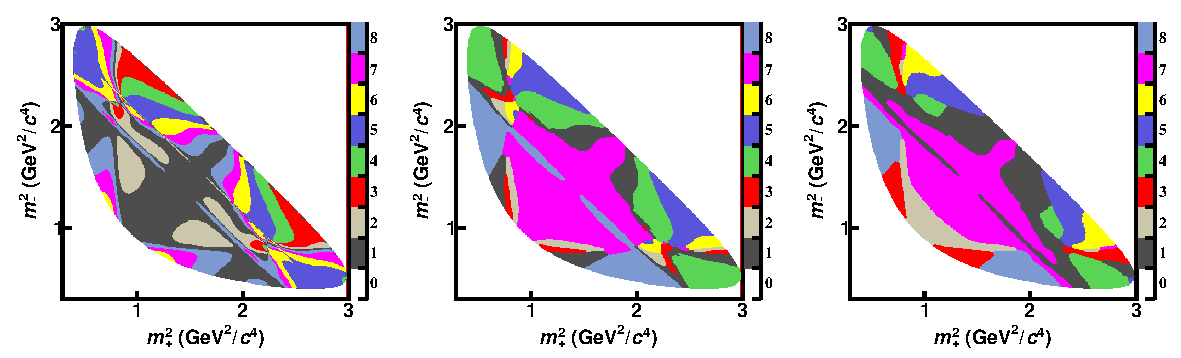
\includegraphics[height=4cm,trim={0 0 14cm 0},clip=true]{Plots/KSpipi_BinningScheme.pdf}
      \caption{Equal $\delta$ binning scheme}
    \end{subfigure}%
    \begin{subfigure}{0.67\textwidth}
      \centering
      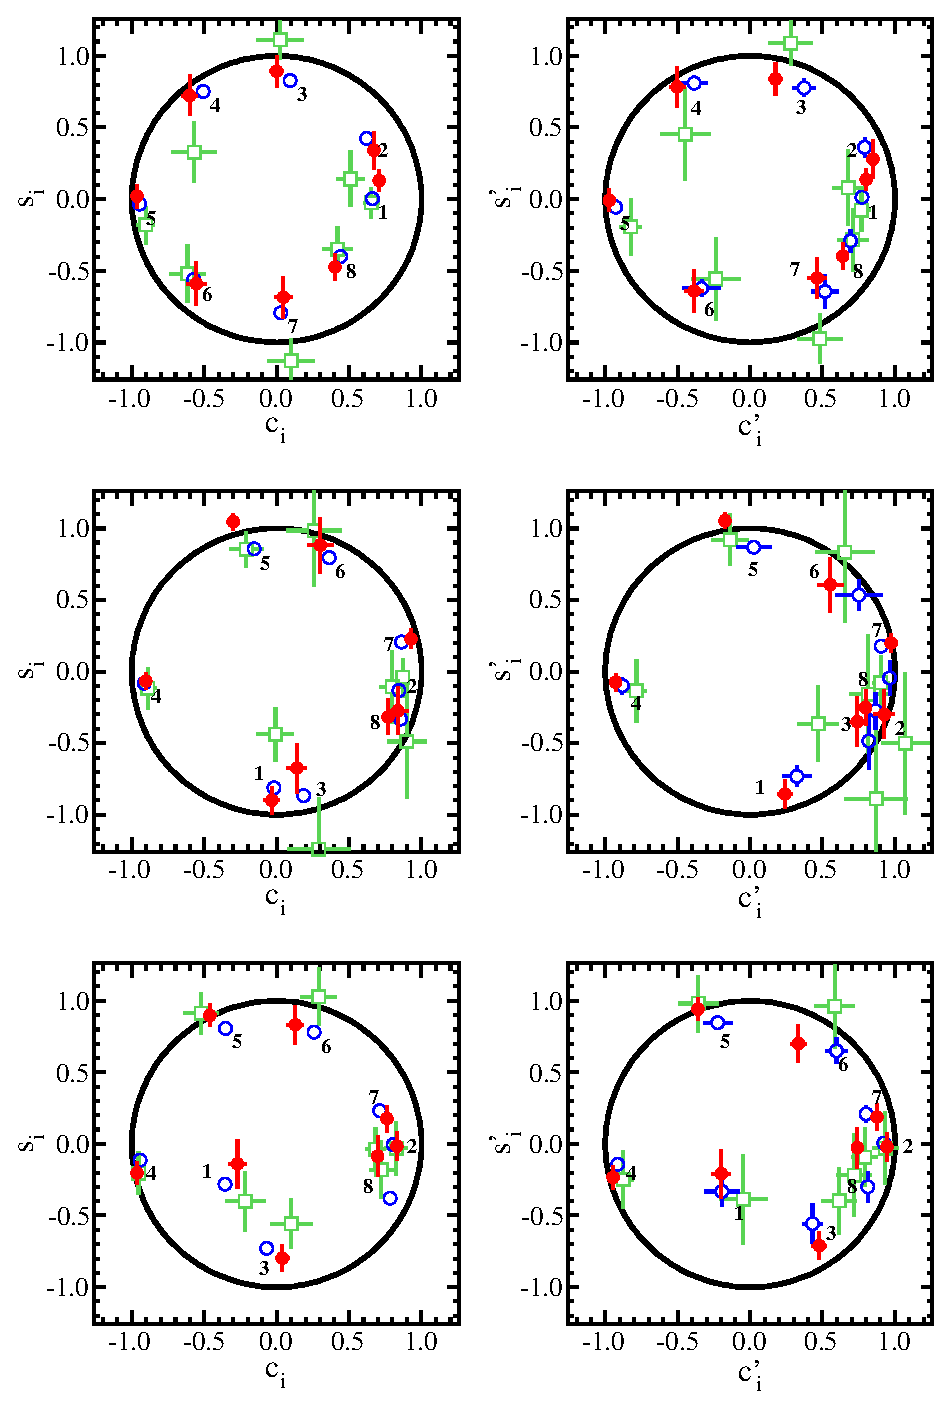
\includegraphics[height=3.8cm,trim={0 16.5cm 0 0},clip=true]{Plots/KSpipi_cisi.pdf}
      \caption{$c_i$ and $s_i$ for (left) $K_S\pi\pi$ and (right) $K_L\pi\pi$}
    \end{subfigure}
  \end{figure}
\end{frame}

\begin{frame}{Introduction - Previous strong-phase analyses}
  \begin{itemize}
    \setlength\itemsep{1.0em}
    \item{Four-body decays have a 5D phase space, but their binning scheme may be defined analogously}
    \item{Many different strategies for 5D binning schemes:}
    \begin{itemize}
      \item{$D\to K_S^0\pi^+\pi^-\pi^0$: \href{https://link.springer.com/article/10.1007/JHEP01(2018)082}{JHEP \textbf{2018} 82 (2018)}}
      \item{$D\to\pi^+\pi^-\pi^+\pi^-$: \href{https://link.springer.com/article/10.1007/JHEP01(2018)144}{JHEP \textbf{2018} 144 (2018)}}
      \item{$D\to K^-\pi^+\pi^-\pi^+$: \href{https://link.springer.com/article/10.1007/JHEP05(2021)164}{JHEP \textbf{2021} 164 (2021)}}
    \end{itemize}
  \end{itemize}
  \begin{figure}
    \centering
    \begin{subfigure}{0.30\textwidth}
      \centering
      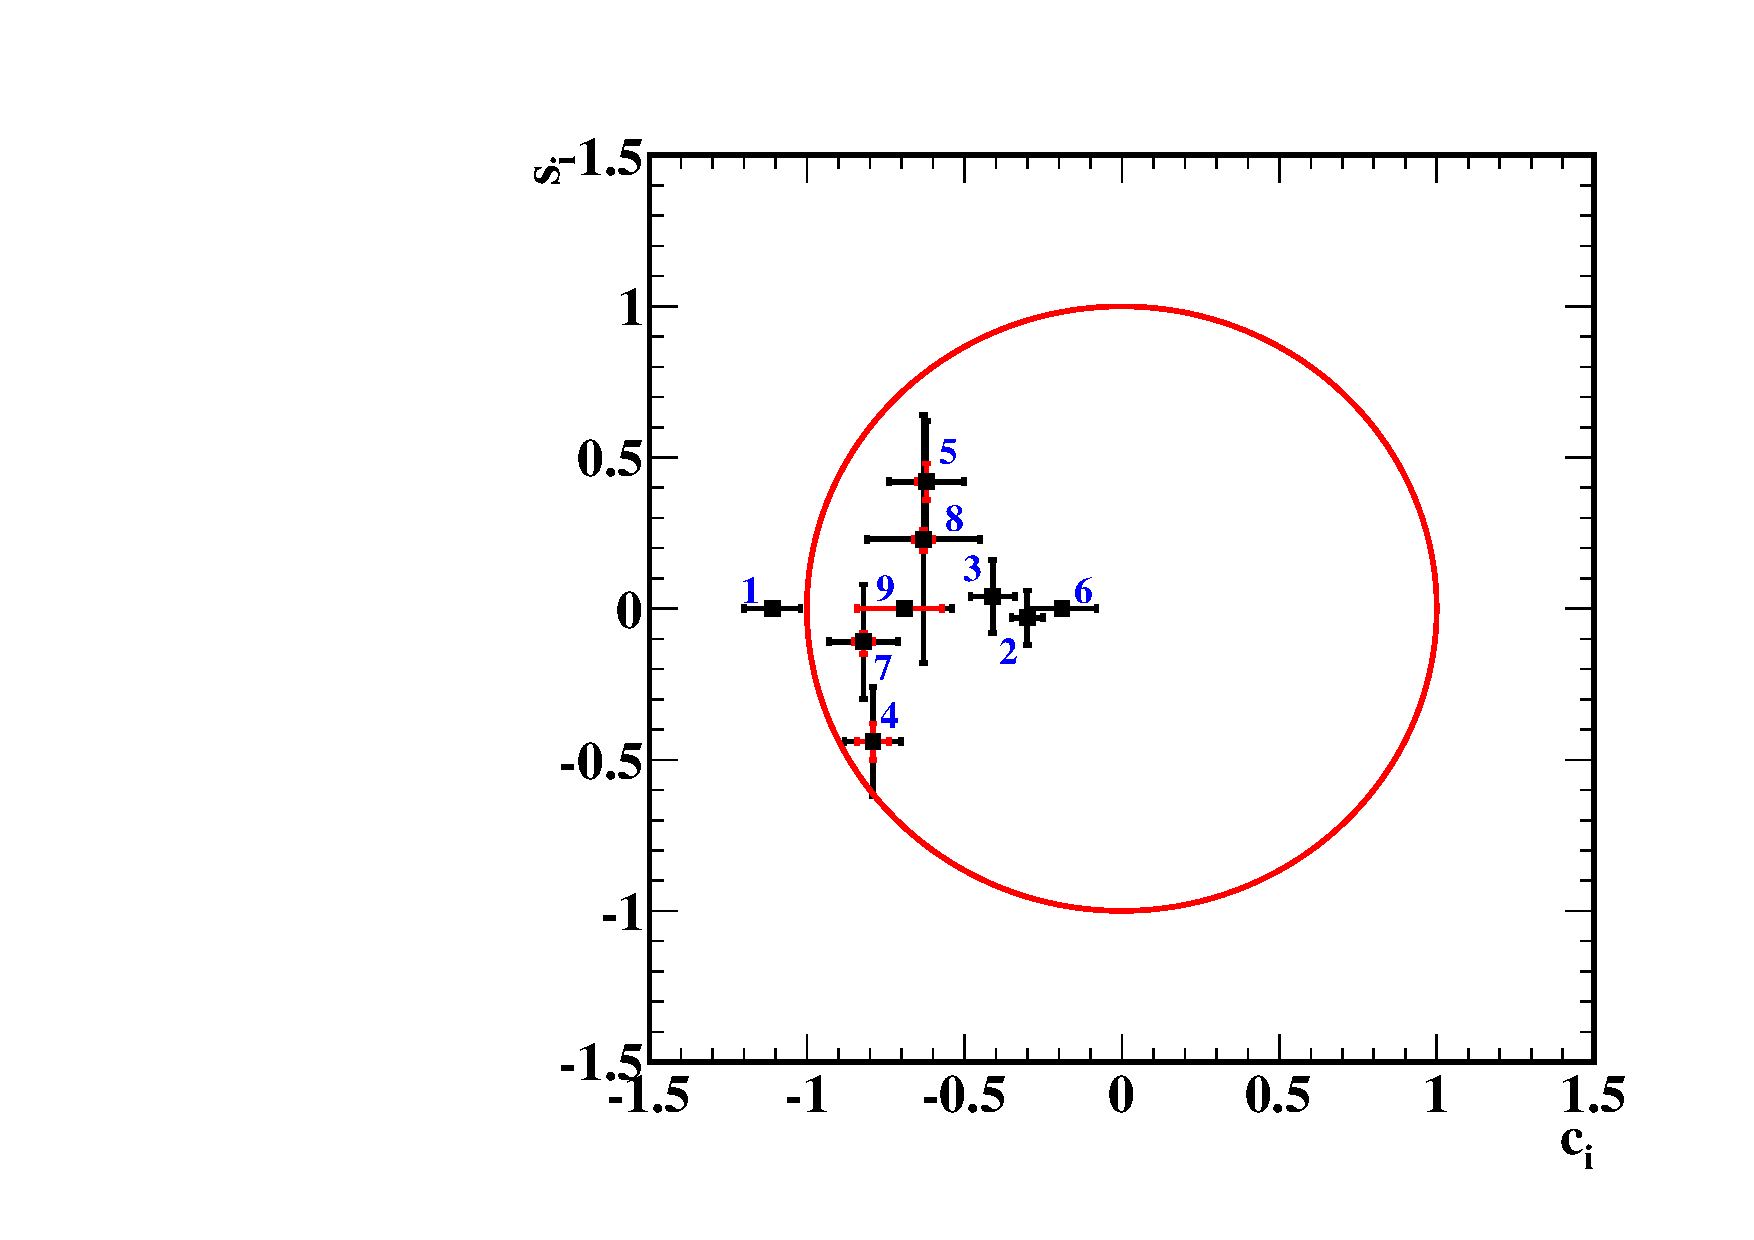
\includegraphics[width=1.0\textwidth]{Plots/KSpipipi0_cisi.pdf}
      \caption{$K_S\pi\pi\pi^0$}
    \end{subfigure}%
    \begin{subfigure}{0.39\textwidth}
      \centering
      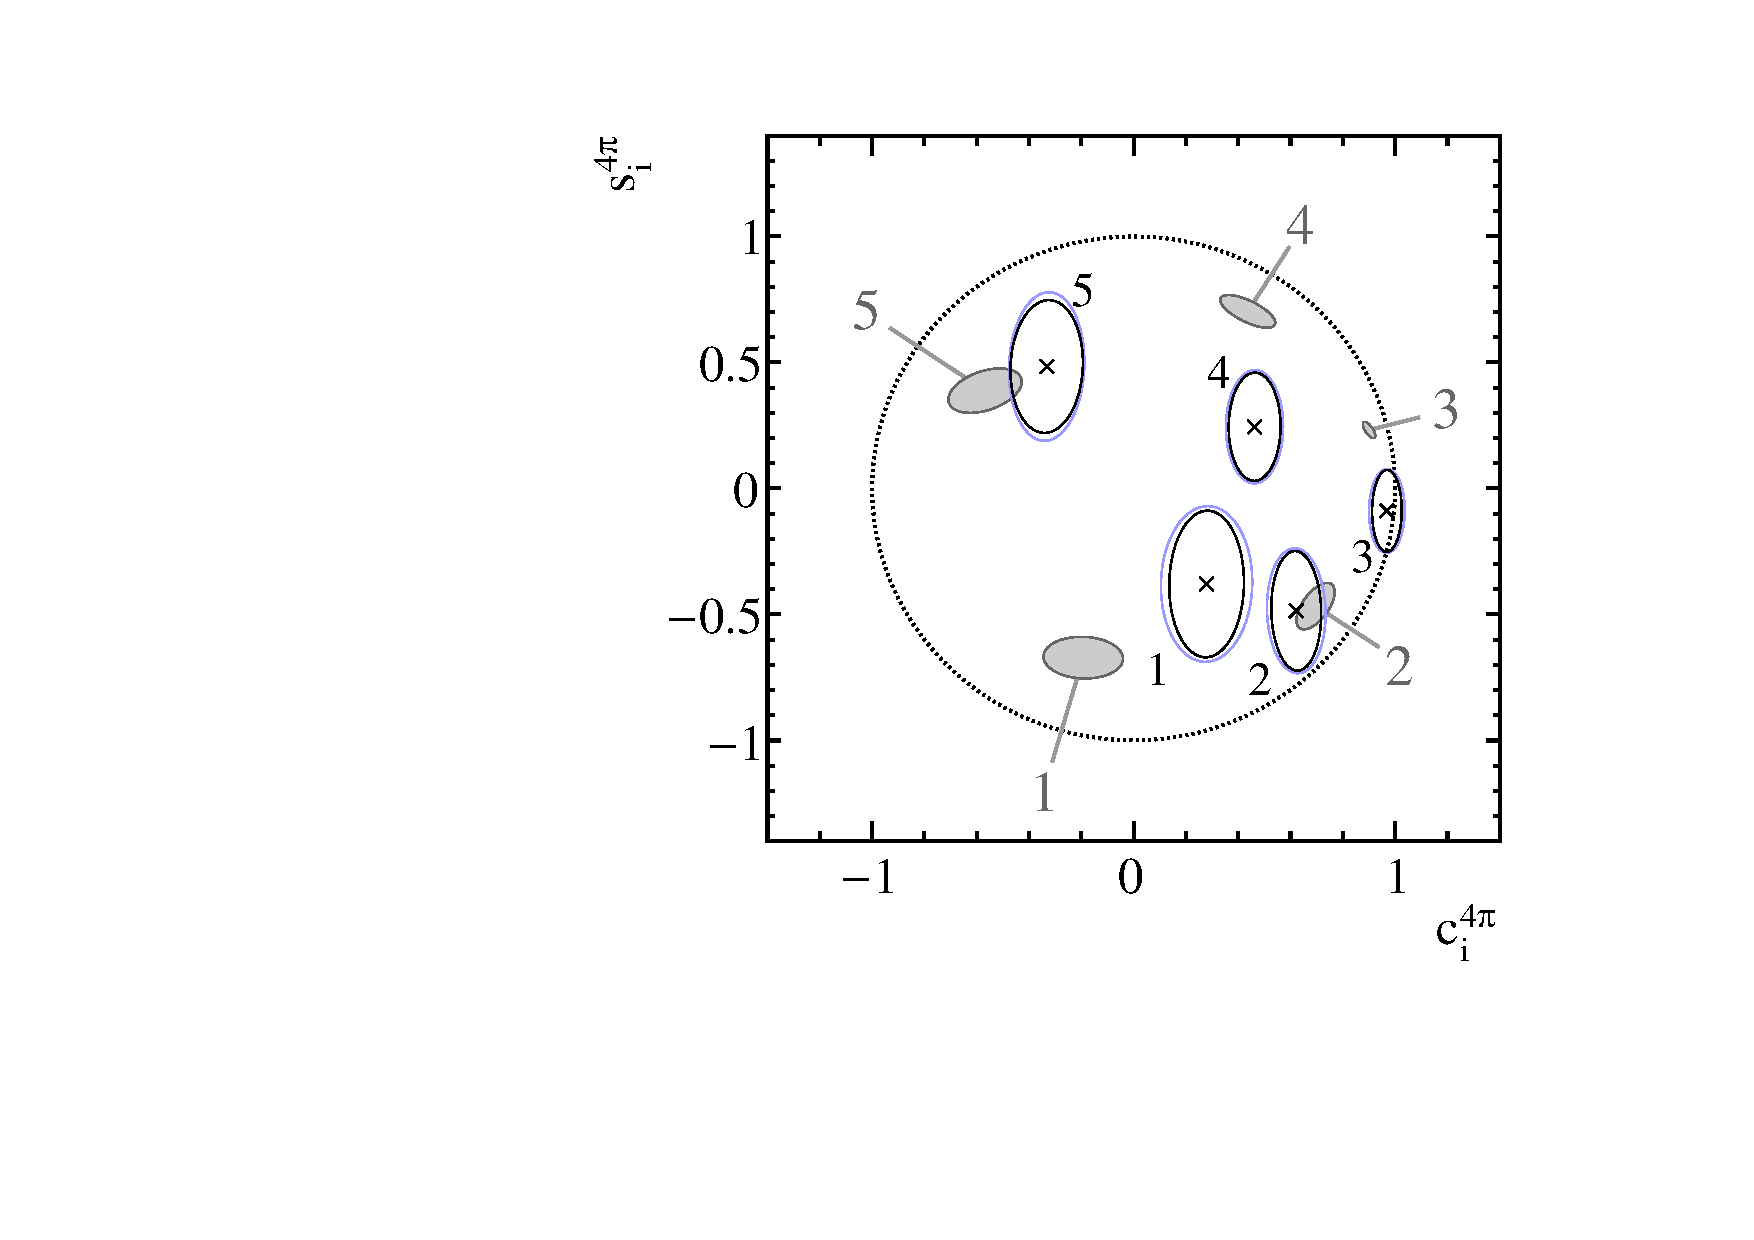
\includegraphics[width=1.0\textwidth,trim={0 0.2cm 0 0},clip=true]{Plots/4pi_cisi.pdf}
      \caption{$4\pi$}
    \end{subfigure}%
    \begin{subfigure}{0.30\textwidth}
      \centering
      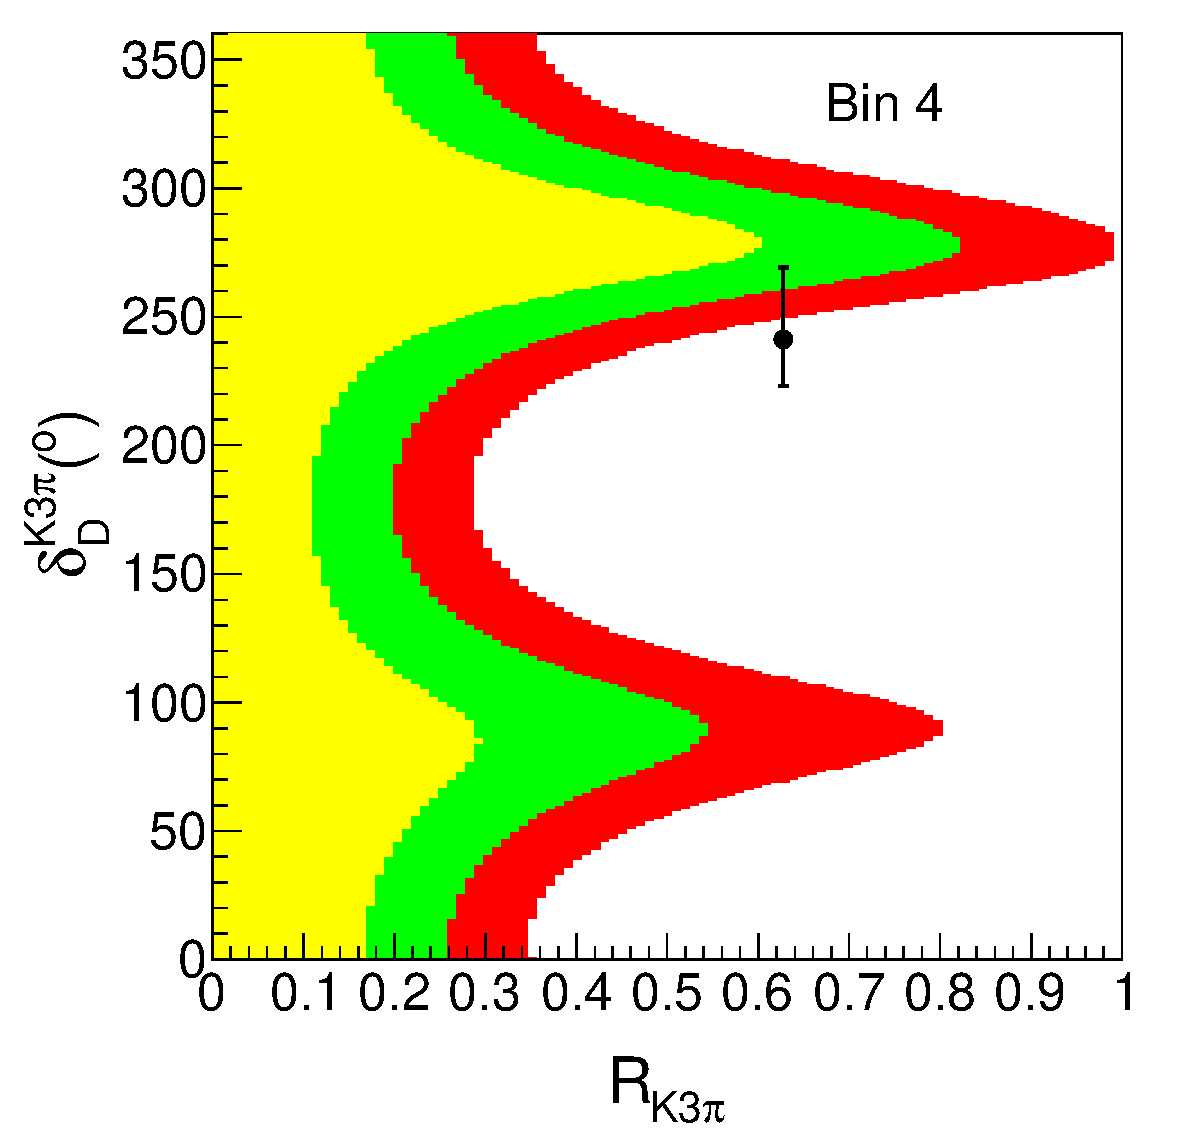
\includegraphics[width=1.0\textwidth,trim={0 0.15cm 0 0},clip=true]{Plots/K3pi_bin4.pdf}
      \caption{$K\pi\pi\pi$}
    \end{subfigure}
  \end{figure}
\end{frame}

\begin{frame}{Introduction - Previous strong-phase analyses}
  \begin{itemize}
    \setlength\itemsep{1.0em}
    \item{The phase-space integrated strong phase of $D\to K^+K^-\pi^+\pi^-$ was previously measured: \href{https://journals.aps.org/prd/abstract/10.1103/PhysRevD.107.032009}{Phys. Rev. D \textbf{107} 032009}}
    \item{The asymmetry in the branching fraction measured using CP even and CP odd tags is sensitive to the CP-even fraction $F_+$}
    \begin{itemize}
      \item{$c_i = 2F_+ - 1$ is the amplitude-average cosine of the strong phase}
    \end{itemize}
  \end{itemize}
  \begin{figure}
    \centering
    \begin{subfigure}{0.50\textwidth}
      \centering
      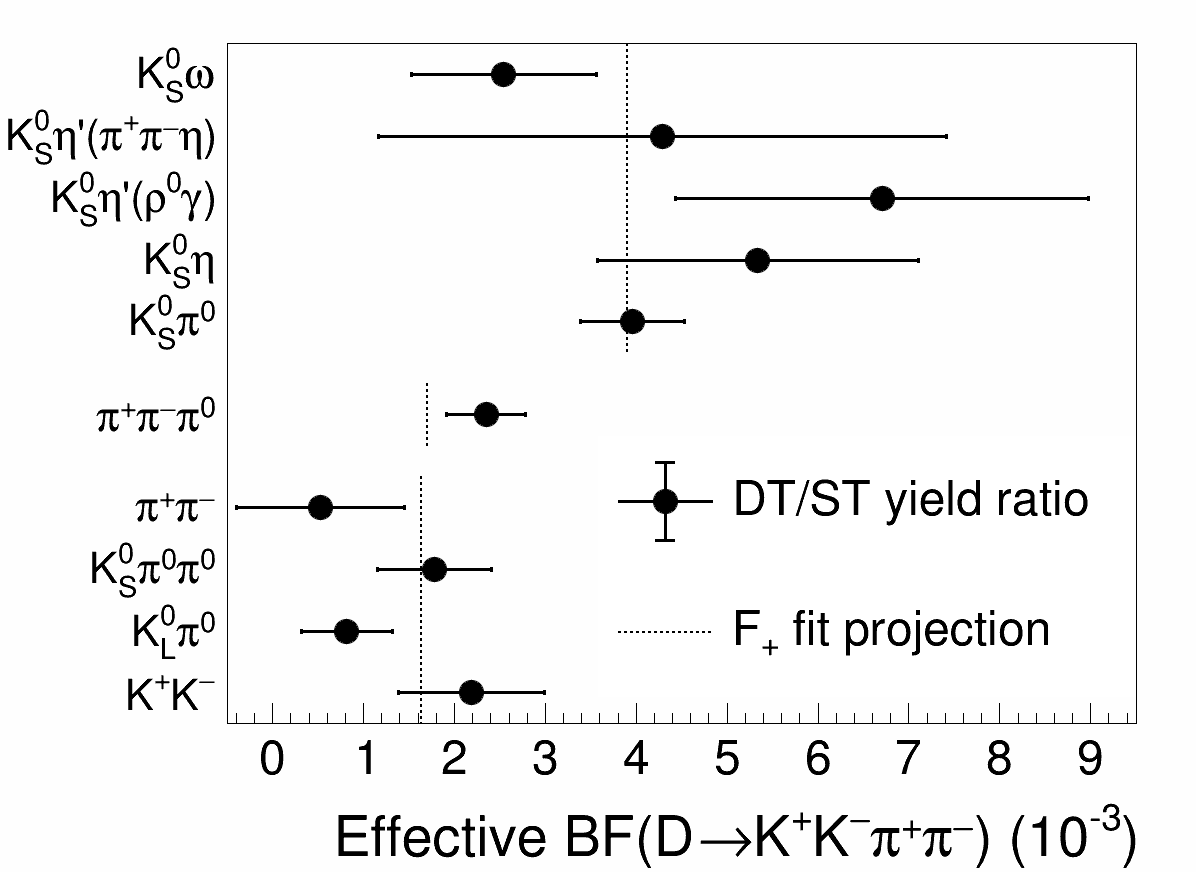
\includegraphics[width=1.0\textwidth]{Plots/CPeven_fraction_combination_CPtags.png}
      \caption{BF asymmetry}
    \end{subfigure}%
    \begin{subfigure}{0.50\textwidth}
      \centering
      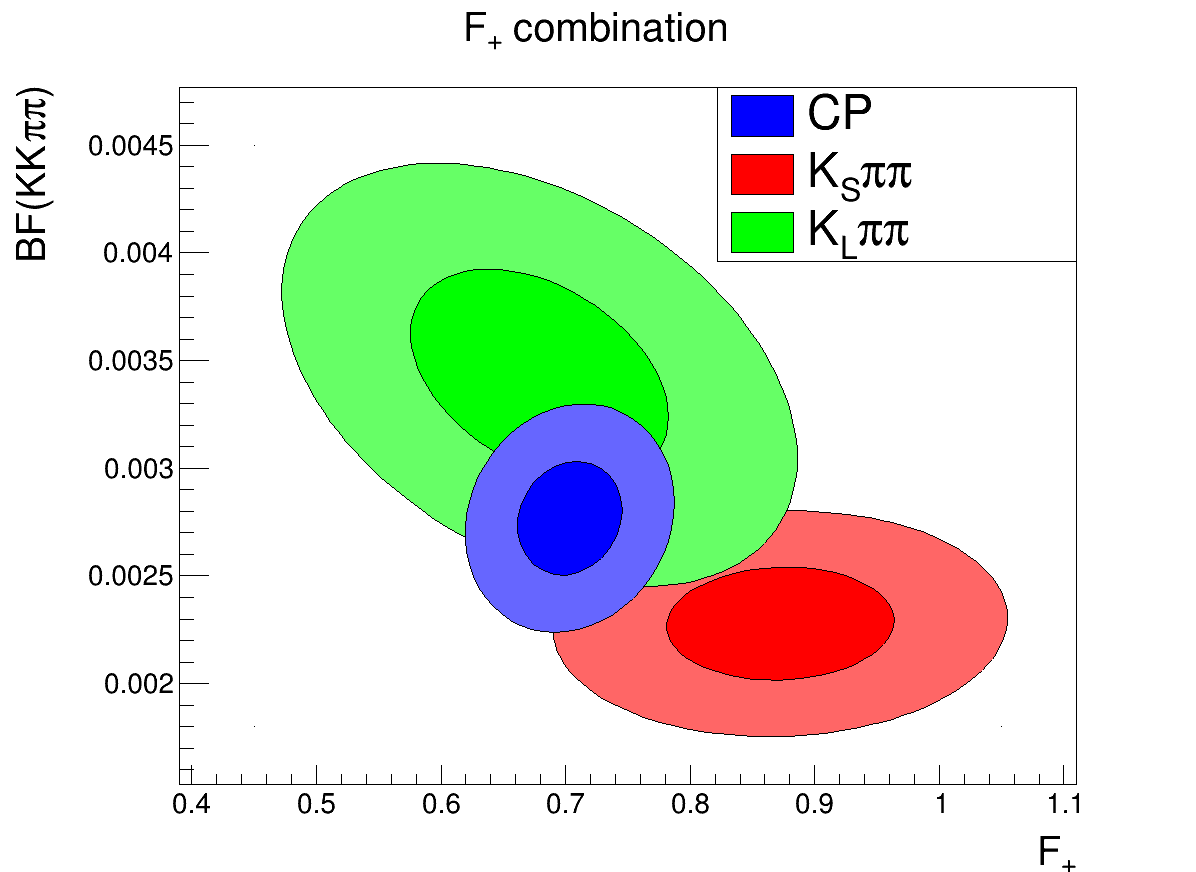
\includegraphics[width=1.0\textwidth,trim={0 0 0 3.0cm},clip=true]{Plots/FPlus_contours.png}
      \caption{$F_+$ combination}
    \end{subfigure}
  \end{figure}
\end{frame}

\section{Binning scheme}
\begin{frame}{Binning scheme}
  \vspace{0.0cm}
  {\Large Strong phases are determined from yield asymmetries}
  \begin{itemize}
    \item{When integrating over a phase-space region, variations in strong phases dilute the asymmetries}
    \item{We require a binning scheme to minimise the dilution and enhance asymmetry effects}
  \end{itemize}
  \vspace{0.4cm}
  {\Large How to bin a 5-dimensional phase space?}
  \begin{itemize}
    \item{Generate C++ code for LHCb amplitude model using AmpGen\footnote{\href{https://github.com/GooFit/AmpGen}{AmpGen} by Tim Evans}}
    \item{For each $D$ event, calculate}
  \end{itemize}
  \begin{center}
    {\Large $\frac{\mathcal{A}(D^0)}{\mathcal{A}(\bar{D^0})} = r_De^{i\delta_D}$}
  \end{center}
  \begin{itemize}
    \item{Bin along $\delta_D$ and $r_D$}
    \begin{itemize}
      \item{Bin boundaries in $\delta_D$ are moved to maximise sensitivity to $\gamma$}
    \end{itemize}
  \end{itemize}
\end{frame}

\begin{frame}{Binning scheme}
  \begin{figure}
    \centering
    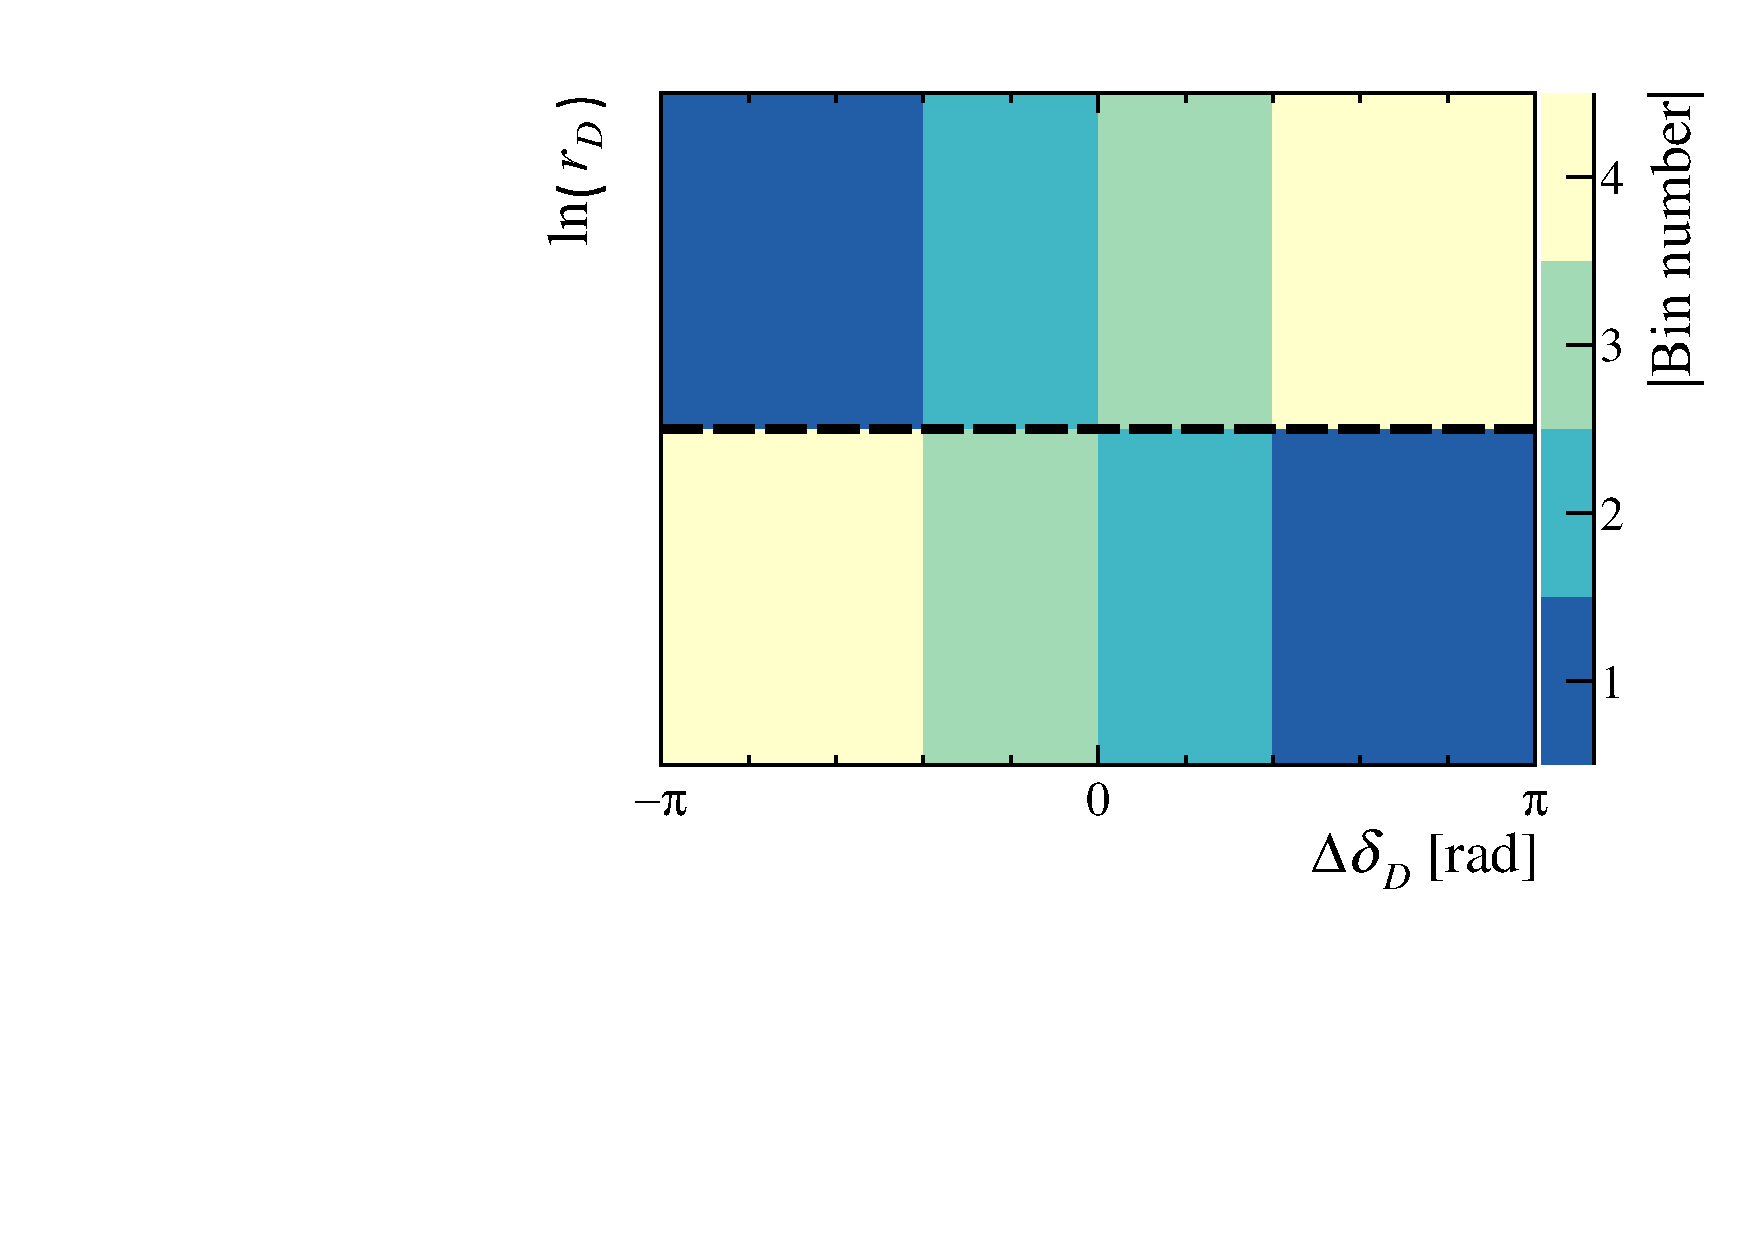
\includegraphics[width = 0.7\textwidth]{Plots/BinningSchemePlot_4Bins.pdf}
  \end{figure}
  \begin{center}
    Bins $i < 0$ on top, $i > 0$ below\\
    Binning scheme used in \underline{this} analysis
  \end{center}
\end{frame}

\begin{frame}{Binning scheme}
  \begin{figure}
    \centering
    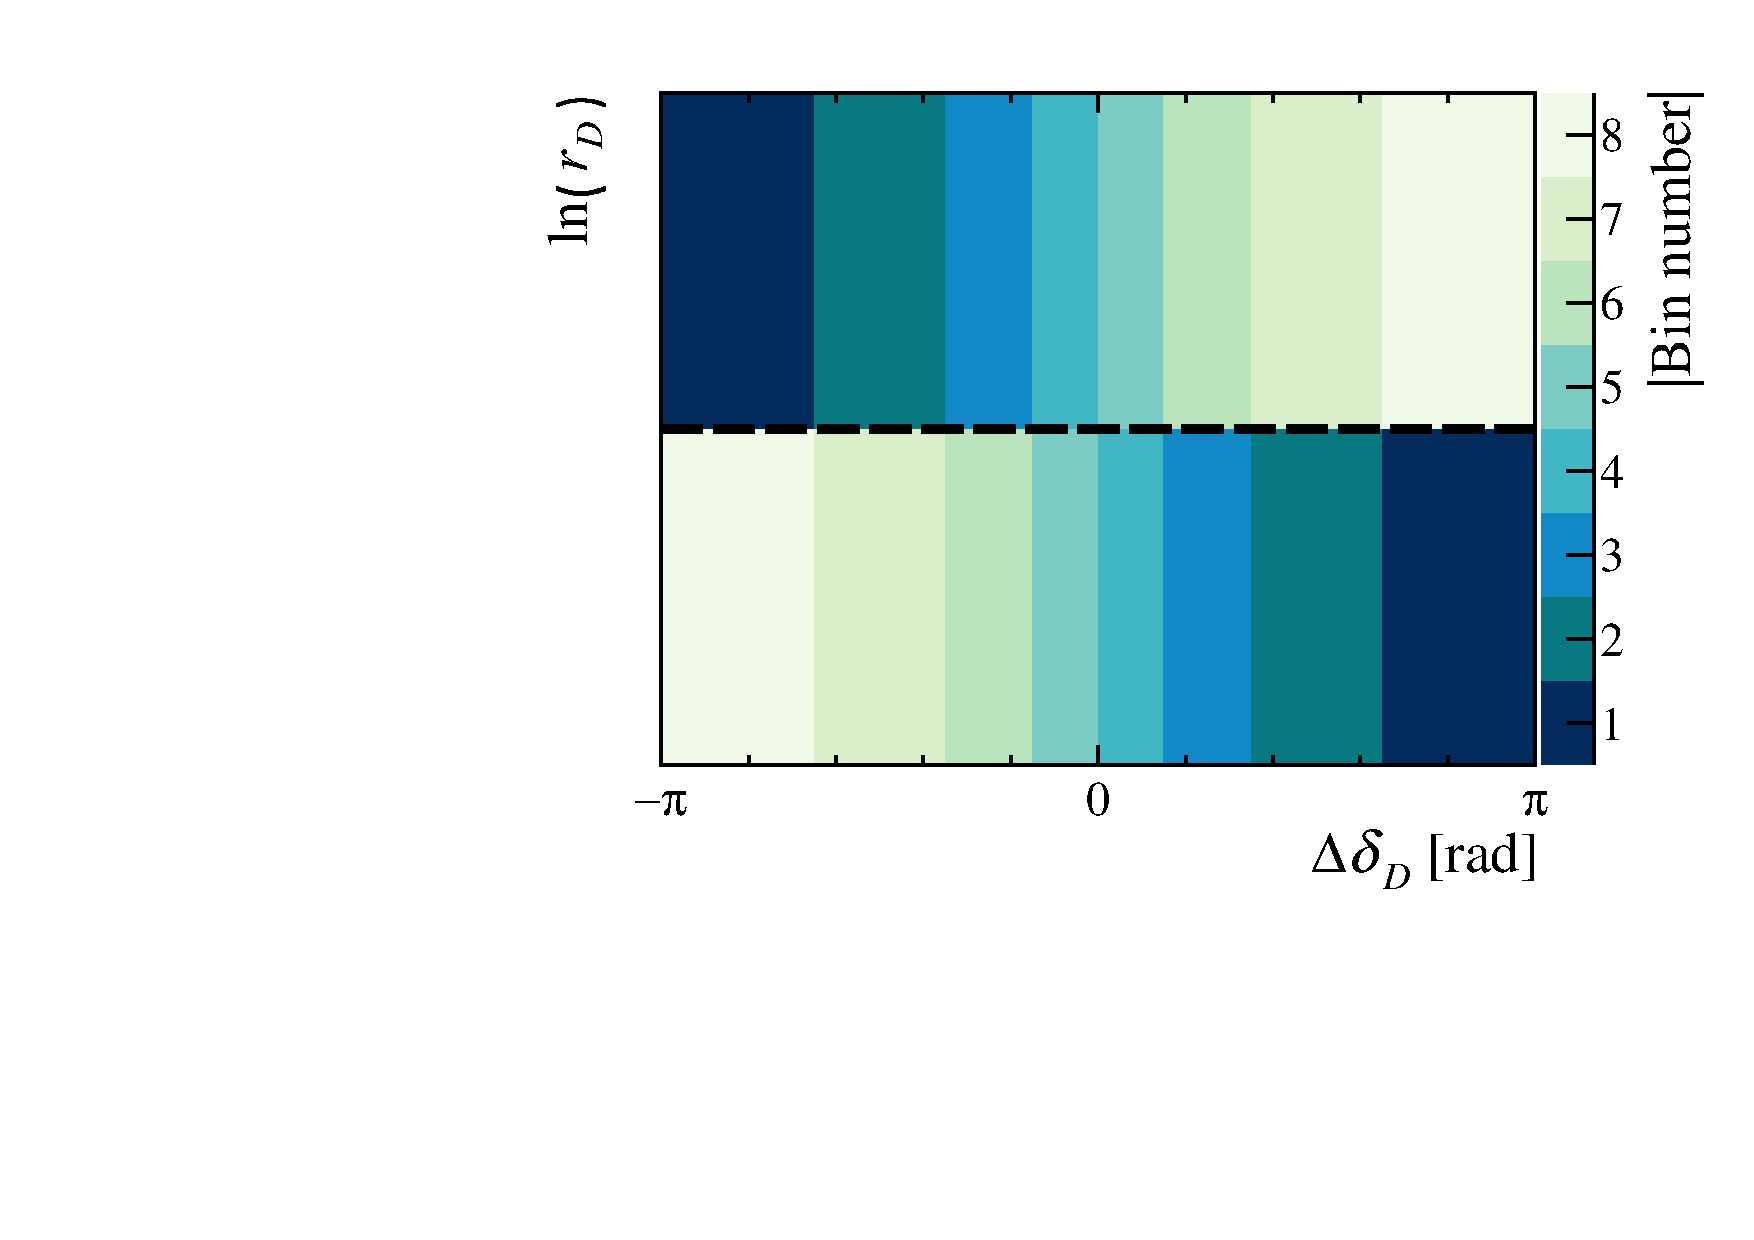
\includegraphics[width = 0.7\textwidth]{Plots/BinningSchemePlot_8Bins.pdf}
  \end{figure}
  \begin{center}
    Bins $i < 0$ on top, $i > 0$ below\\
    Possible binning scheme for future analysis with $\SI{20}{\per\femto\barn}$ dataset
  \end{center}
\end{frame}

\section{Model-dependent measurement at LHCb}
\begin{frame}{Model-dependent measurement at LHCb}
  \begin{figure}
    \centering
    \begin{subfigure}{0.50\textwidth}
      \centering
      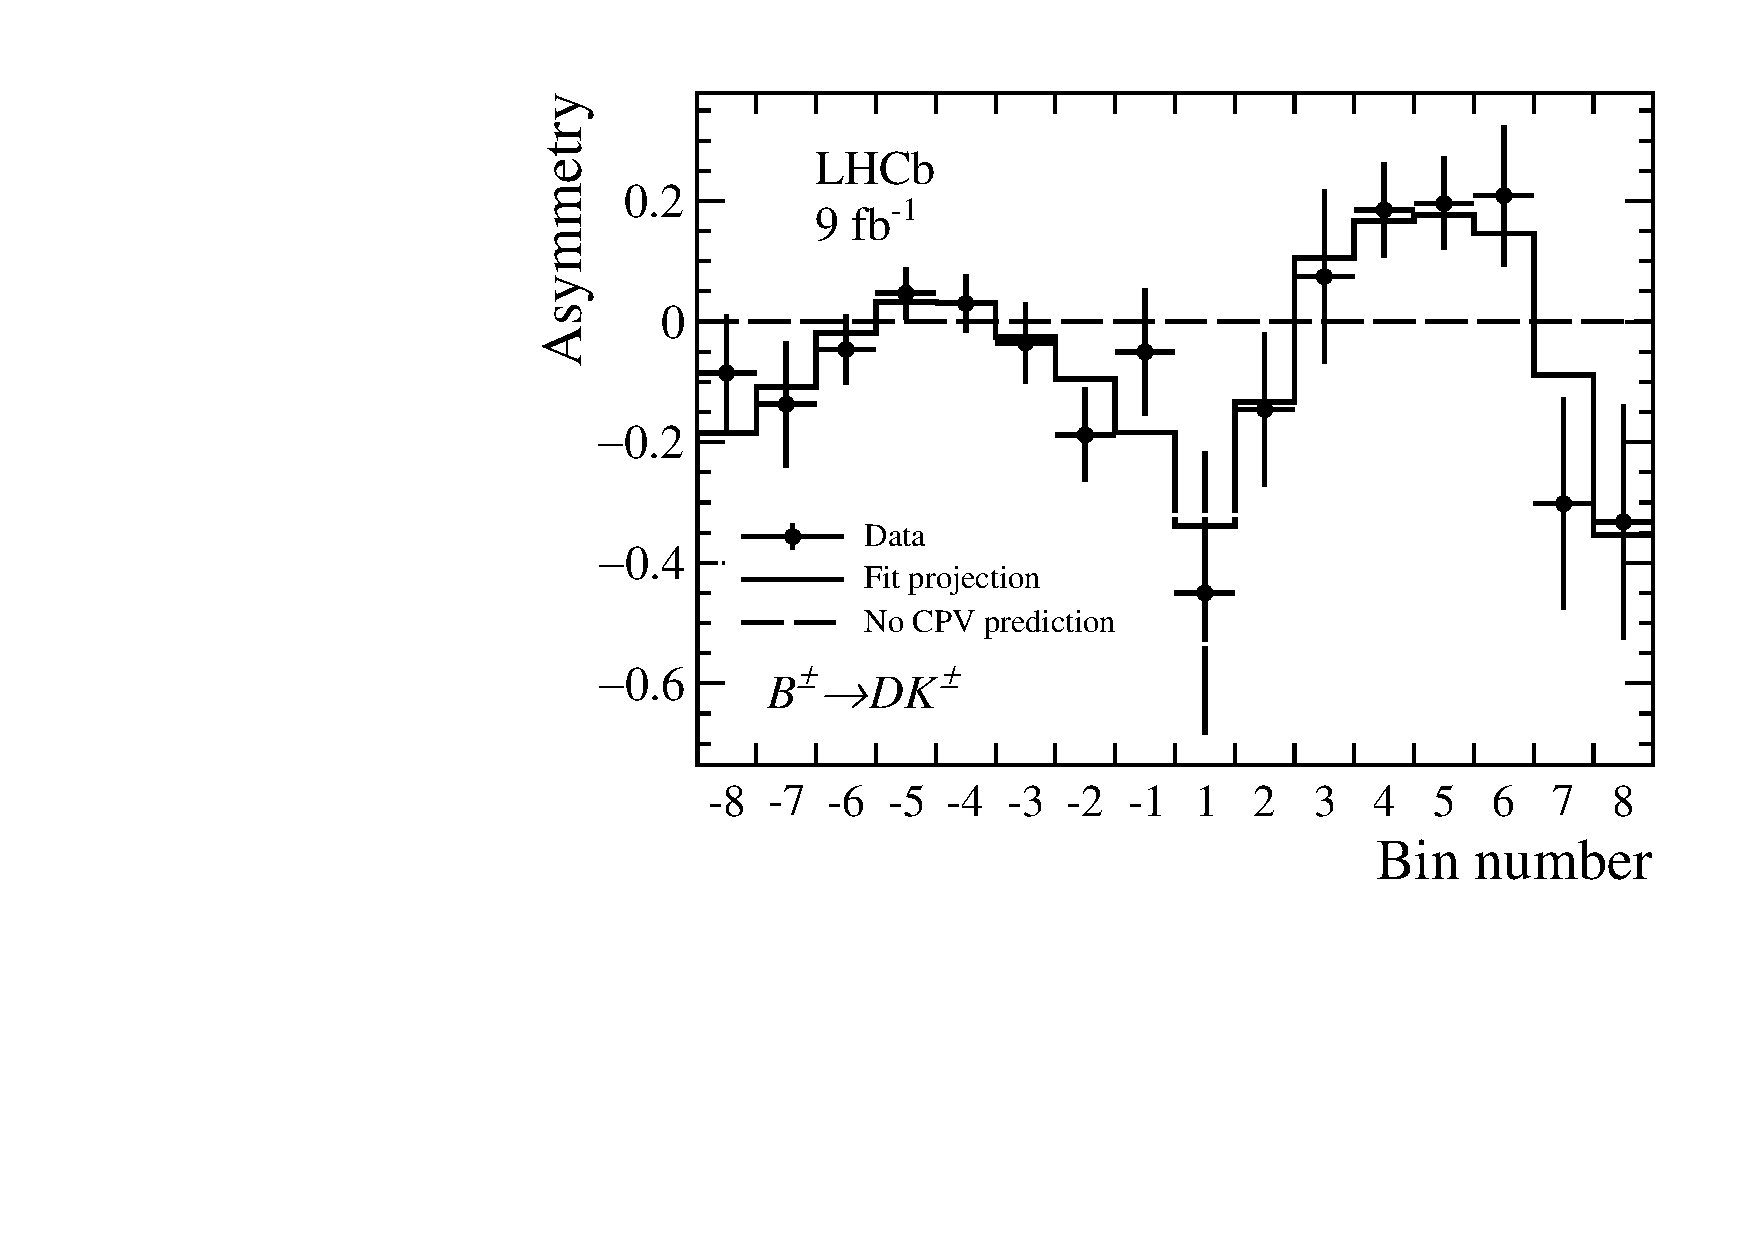
\includegraphics[width=1.0\textwidth]{Plots/BinAsymmetries_dk.pdf}
      \caption{Bin asymmetries in $B^\pm\to DK^\pm$}
    \end{subfigure}%
    \begin{subfigure}{0.50\textwidth}
      \centering
      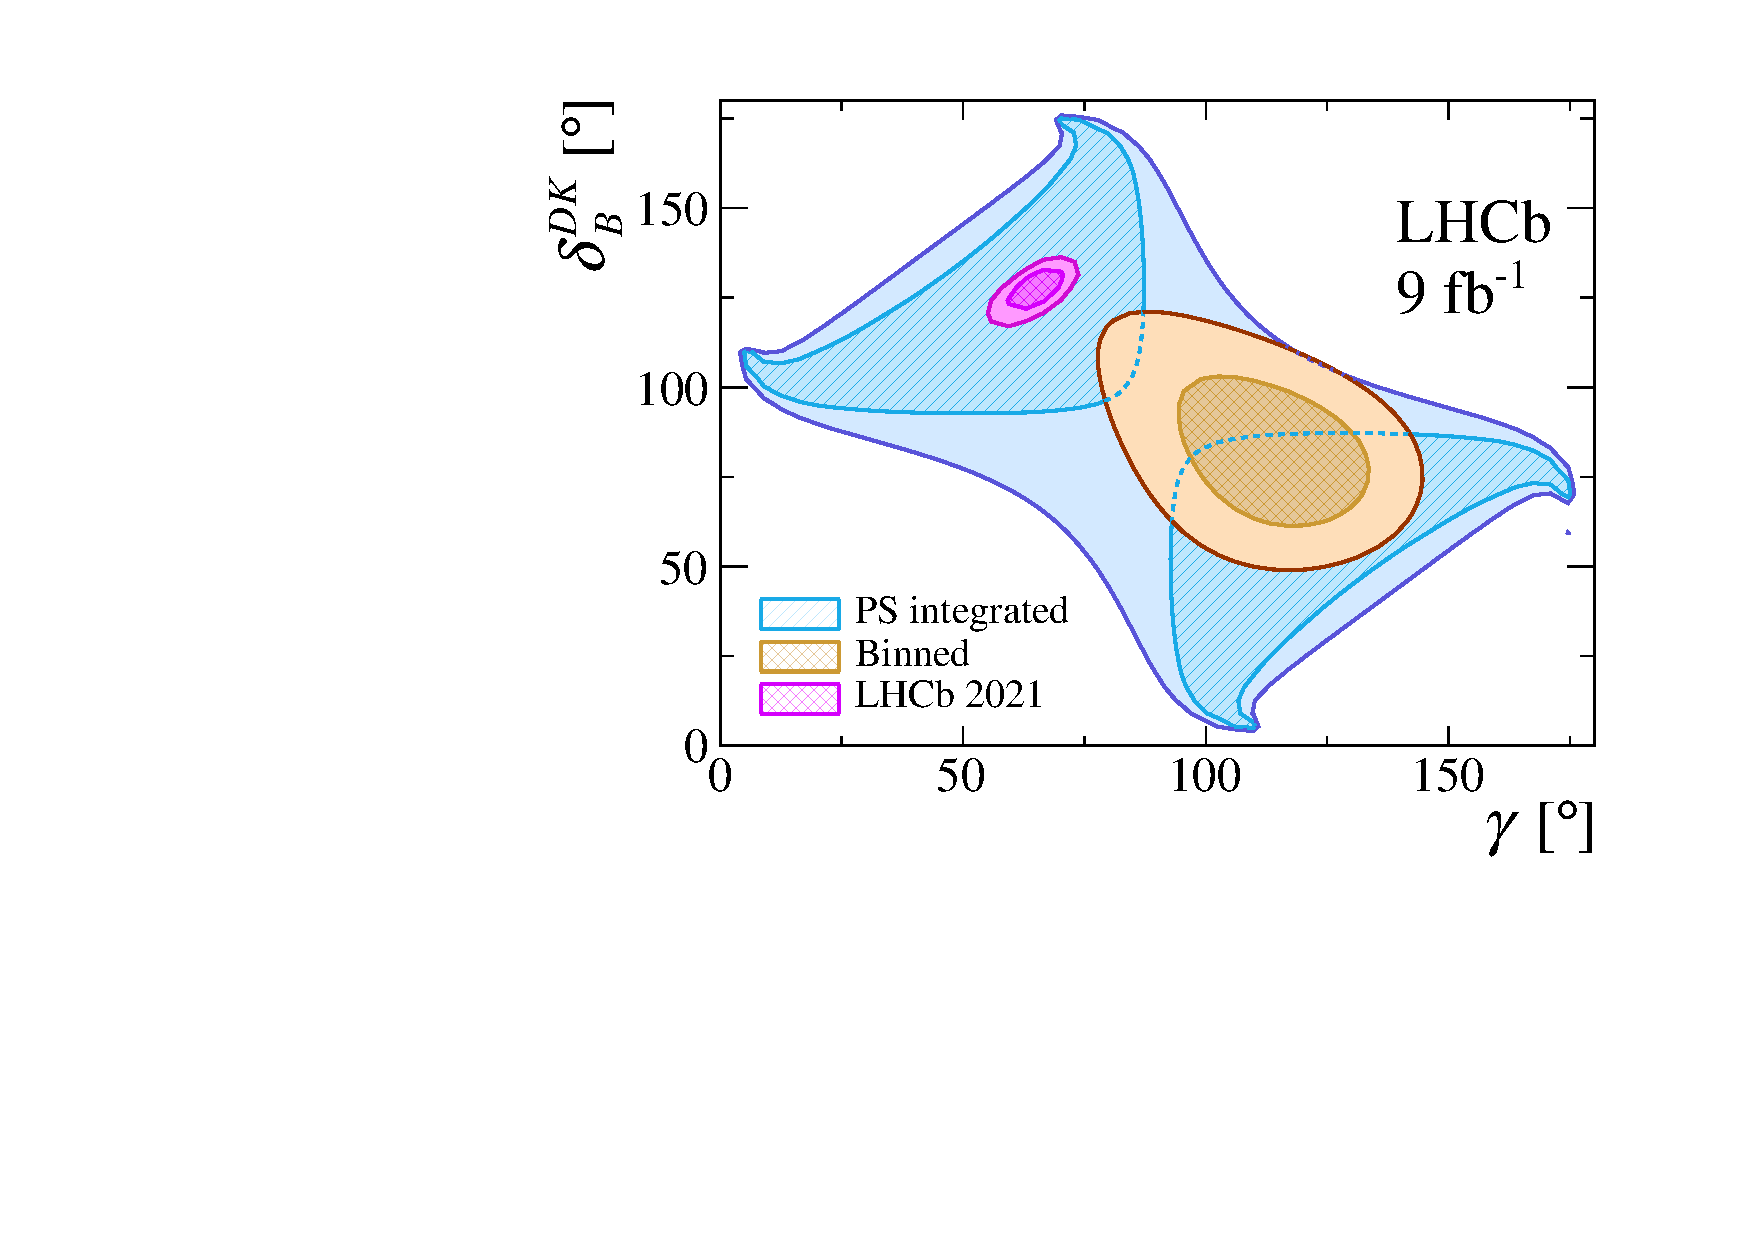
\includegraphics[width=1.0\textwidth,trim={0 0.15cm 0 0},clip=true]{Plots/gammacharm_lhcb_KKpipi_GLW_KKpipi_GGSZ_lhcb_2020_beauty_and_charm_g_d_dk.pdf}
      \caption{Measurement of $\gamma$ at LHCb}
    \end{subfigure}
  \end{figure}
  \begin{center}
    $\gamma = (116^{+12}_{-14})^\circ$\\~\\
    This result is currently model independent, and needs external inputs from BESIII to become a proper model-independent measurement!
  \end{center}
\end{frame}

\section{Formalism and measurement strategy}
\begin{frame}{Formalism and measurement strategy}
  \vspace{0.0cm}
  {\Large $D\bar{D}$ pair from $\psi(3770)$ is prepared in a $\mathcal{C} = -1$ state}
  \vspace{0.5cm}
  \begin{itemize}
    \setlength\itemsep{1.0em}
    \item{$D$ mesons are ``quantum correlated''}
    \item{The decay of $D\to K^+K^-\pi^+\pi^-$ is correlated by the $C\!P$ content of the tag mode}
  \end{itemize}
  \begin{center}
    $\lvert D\bar{D}\rangle = \frac{1}{\sqrt{2}}\big(\lvert D^0\rangle\lvert\bar{D^0}\rangle - \lvert\bar{D^0}\rangle\lvert D^0\rangle\big)$
  \end{center}
  \begin{itemize}
    \item{Equivalently, in terms of $C\!P$ eigenstates:}
  \end{itemize}
  \begin{center}
    $\lvert D\bar{D}\rangle = \frac{1}{\sqrt{2}}\big(\lvert D_-\rangle\lvert D_+\rangle - \lvert D_+\rangle\lvert D_-\rangle\big)$
  \end{center}
\end{frame}

\begin{frame}{Formalism and measurement strategy}
  \begin{itemize}
    \item{Tag mode can be a \underline{flavour tag}}
    \begin{itemize}
      \item{$K\pi$, $K\pi\pi^0$, $K\pi\pi\pi$, $Ke\nu$}
    \end{itemize}
  \end{itemize}
  \begin{figure}[H]
    \centering
    \vspace{0.3cm}
    \begin{fmffile}{fgraph/fgraph_flavour_tag}
      \setlength{\unitlength}{1cm}
      \begin{fmfgraph*}(8,4)
        \fmfstraight
        \fmfleft{i4,i3,i2,i1}
        \fmfright{g1,o1,o2,g2}
        \fmflabel{$\pi^+$}{o1}
        \fmflabel{$K^-$}{o2}
        \fmflabel{$K^+$}{i1}
        \fmflabel{$K^-$}{i2}
        \fmflabel{$\pi^+$}{i3}
        \fmflabel{$\pi^-$}{i4}
        \fmf{plain}{w,i1}
        \fmf{plain}{w,i2}
        \fmf{plain}{w,i3}
        \fmf{plain}{w,i4}
        \fmf{plain}{w,o1}
        \fmf{plain}{w,o2}
        \fmf{phantom}{w,g1}
        \fmf{phantom}{w,g2}
        \fmfblob{1cm}{w}
      \end{fmfgraph*}
    \end{fmffile}
    \vspace{0.3cm}
  \end{figure}
  \begin{center}
    Use flavour tags to measure fraction of $D^0\to KK\pi\pi$ decays in bin $i$:\\
    $\frac{N^{\rm DT}_i}{N^{\rm ST}} = \mathcal{B}\times K_i$
  \end{center}
\end{frame}

\begin{frame}{Formalism and measurement strategy}
  \begin{itemize}
    \item{Tag mode can be a \underline{CP even tag}}
    \begin{itemize}
      \item{$KK$ (fully and part. reco $KK\pi\pi$), $\pi\pi$, $\pi\pi\pi^0$, $K_S\pi^0\pi^0$, $K_L\pi^0$}
    \end{itemize}
  \end{itemize}
  \begin{figure}[H]
    \centering
    \vspace{0.3cm}
    \begin{fmffile}{fgraph/fgraph_CPeven_tag}
      \setlength{\unitlength}{1cm}
      \begin{fmfgraph*}(8,4)
        \fmfstraight
        \fmfleft{i4,i3,i2,i1}
        \fmfright{g1,o1,o2,g2}
        \fmflabel{$K^+$}{o1}
        \fmflabel{$K^-$}{o2}
        \fmflabel{$K^+$}{i1}
        \fmflabel{$K^-$}{i2}
        \fmflabel{$\pi^+$}{i3}
        \fmflabel{$\pi^-$}{i4}
        \fmf{plain}{w,i1}
        \fmf{plain}{w,i2}
        \fmf{plain}{w,i3}
        \fmf{plain}{w,i4}
        \fmf{plain}{w,o1}
        \fmf{plain}{w,o2}
        \fmf{phantom}{w,g1}
        \fmf{phantom}{w,g2}
        \fmfblob{1cm}{w}
      \end{fmfgraph*}
    \end{fmffile}
    \vspace{0.3cm}
  \end{figure}
  \begin{center}
    $D\to K^+K^-$, which is $C\!P$ even, forces $D\to K^+K^-\pi^+\pi^-$ to be $C\!P$ odd:\\
    $\frac{N^{\rm DT}_i}{N^{\rm ST}} = \mathcal{B}\times(K_i + K_{-i} - 2\sqrt{K_iK_{-i}}c_i)$
  \end{center}
\end{frame}

\begin{frame}{Formalism and measurement strategy}
  \begin{itemize}
    \item{Tag mode can be a \underline{CP odd tag}}
    \begin{itemize}
      \item{$K_S\pi^0$ (fully and part.reco $KK\pi\pi$), $K_S\eta$, $K_S\eta'(\pi\pi\eta, \pi\pi\gamma)$, $K_S\pi\pi\pi^0$}
    \end{itemize}
  \end{itemize}
  \begin{figure}[H]
    \centering
    \vspace{0.3cm}
    \begin{fmffile}{fgraph/fgraph_CPodd_tag}
      \setlength{\unitlength}{1cm}
      \begin{fmfgraph*}(8,4)
        \fmfstraight
        \fmfleft{i4,i3,i2,i1}
        \fmfright{g1,o1,o2,g2}
        \fmflabel{$\pi^0$}{o1}
        \fmflabel{$K_S$}{o2}
        \fmflabel{$K^+$}{i1}
        \fmflabel{$K^-$}{i2}
        \fmflabel{$\pi^+$}{i3}
        \fmflabel{$\pi^-$}{i4}
        \fmf{plain}{w,i1}
        \fmf{plain}{w,i2}
        \fmf{plain}{w,i3}
        \fmf{plain}{w,i4}
        \fmf{plain}{w,o1}
        \fmf{plain}{w,o2}
        \fmf{phantom}{w,g1}
        \fmf{phantom}{w,g2}
        \fmfblob{1cm}{w}
      \end{fmfgraph*}
    \end{fmffile}
    \vspace{0.3cm}
  \end{figure}
  \begin{center}
    $D\to K_S^0\pi^0$, which is $C\!P$ odd, forces $D\to K^+K^-\pi^+\pi^-$ to be $C\!P$ even:\\
    $\frac{N^{\rm DT}_i}{N^{\rm ST}} = \mathcal{B}\times(K_i + K_{-i} + 2\sqrt{K_iK_{-i}}c_i)$
  \end{center}
\end{frame}

\begin{frame}{Formalism and measurement strategy}
  \begin{itemize}
    \item{Tag mode can be a \underline{self-conjugate multi-body tag}}
    \begin{itemize}
      \item{$K_S\pi\pi$ (fully and part.reco $KK\pi\pi$), $K_L\pi\pi$}
    \end{itemize}
  \end{itemize}
  \begin{figure}[H]
    \centering
    \vspace{0.3cm}
    \begin{fmffile}{fgraph/fgraph_SCMB_tag}
      \setlength{\unitlength}{1cm}
      \begin{fmfgraph*}(8,4)
        \fmfstraight
        \fmfleft{i4,i3,i2,i1}
        \fmfright{g1,o1,o2,o3,g2}
        \fmflabel{$\pi^-$}{o1}
        \fmflabel{$\pi^+$}{o2}
        \fmflabel{$K_S$}{o3}
        \fmflabel{$K^+$}{i1}
        \fmflabel{$K^-$}{i2}
        \fmflabel{$\pi^+$}{i3}
        \fmflabel{$\pi^-$}{i4}
        \fmf{plain}{w,i1}
        \fmf{plain}{w,i2}
        \fmf{plain}{w,i3}
        \fmf{plain}{w,i4}
        \fmf{plain}{w,o1}
        \fmf{plain}{w,o2}
        \fmf{plain}{w,o3}
        \fmf{phantom}{w,g1}
        \fmf{phantom}{w,g2}
        \fmfblob{1cm}{w}
      \end{fmfgraph*}
    \end{fmffile}
    \vspace{0.3cm}
  \end{figure}
  \begin{center}
    $D\to K_S^0\pi^+\pi^-$ has different strong phases in different bins of phase space:\\
    $\frac{N^{\rm DT}_{ij}}{N^{\rm ST}} = \mathcal{B}\times\big(K_iK_{-j}^\prime + K_{-i}K_j^\prime - 2\sqrt{K_iK_{-i}K_j^\prime K_{-j}^\prime}(c_ic_j^\prime + s_is_j^\prime)\big)$
  \end{center}
\end{frame}

\section{Selection}
\begin{frame}{Selection}
  \begin{itemize}
    \setlength\itemsep{0.7em}
    \item{Double-tag analysis: Select $D\to KK\pi\pi$ events tagged with flavour, $C\!P$ and multi-body tags}
    \item{Selection more or less identical to previous double-tag analyses}
    \item{$D\to KK\pi\pi$ selection:}
    \begin{itemize}
      \item{$4$ good charged tracks}
      \item{$3\sigma$ window around signal peak in $\Delta E$}
      \item{Asymmetric $K_SKK$ veto for $m(\pi^+\pi^-)\in[477, 507]~\si{\mega\eV}$}
      \item{Flight significance cut at $2$}
    \end{itemize}
  \end{itemize}
  \begin{figure}
    \centering
    \begin{subfigure}{0.5\textwidth}
      \centering
      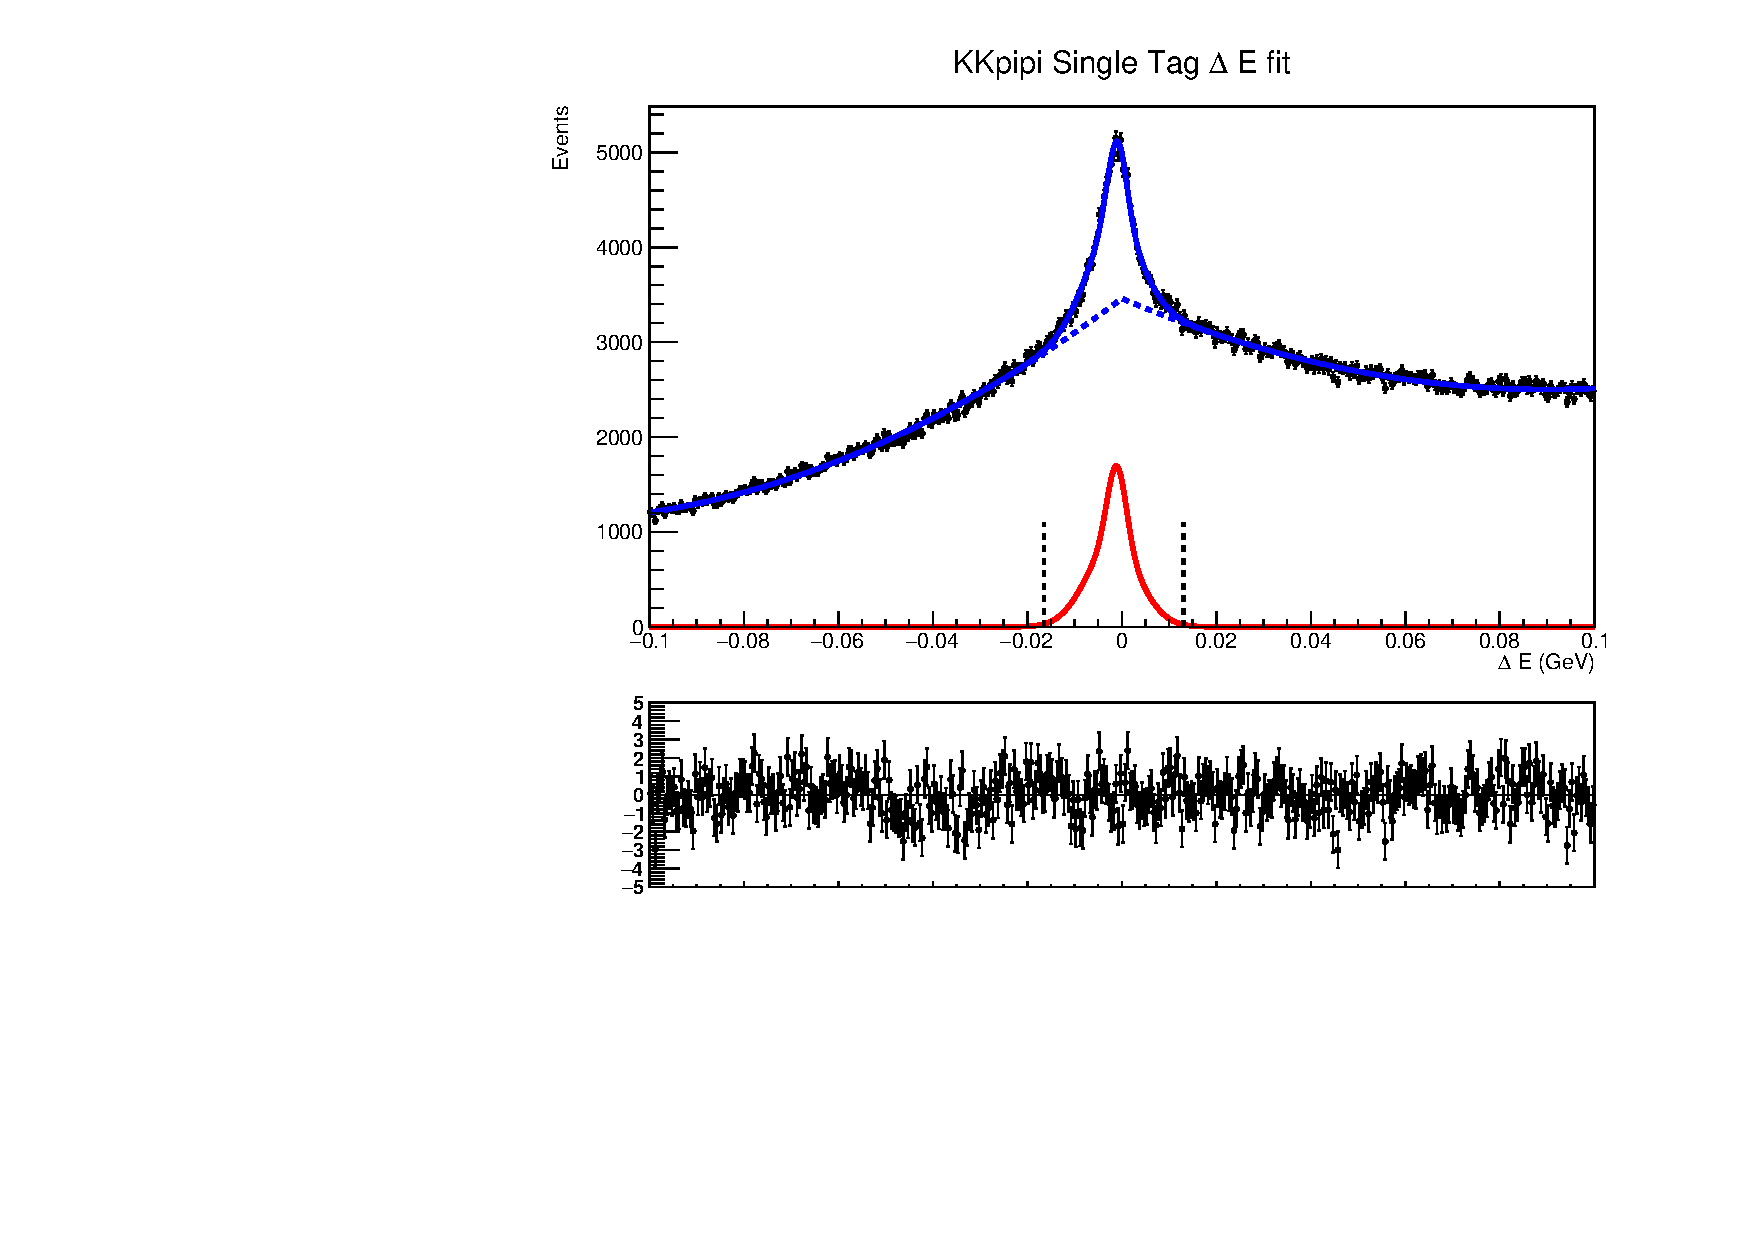
\includegraphics[height=3cm,trim={0 3.8cm 0 0},clip=true]{Plots/KKpipi_SingleTag_DeltaE_Plot.pdf}
      \caption{$\Delta E$ window}
    \end{subfigure}%
    \begin{subfigure}{0.5\textwidth}
      \centering
      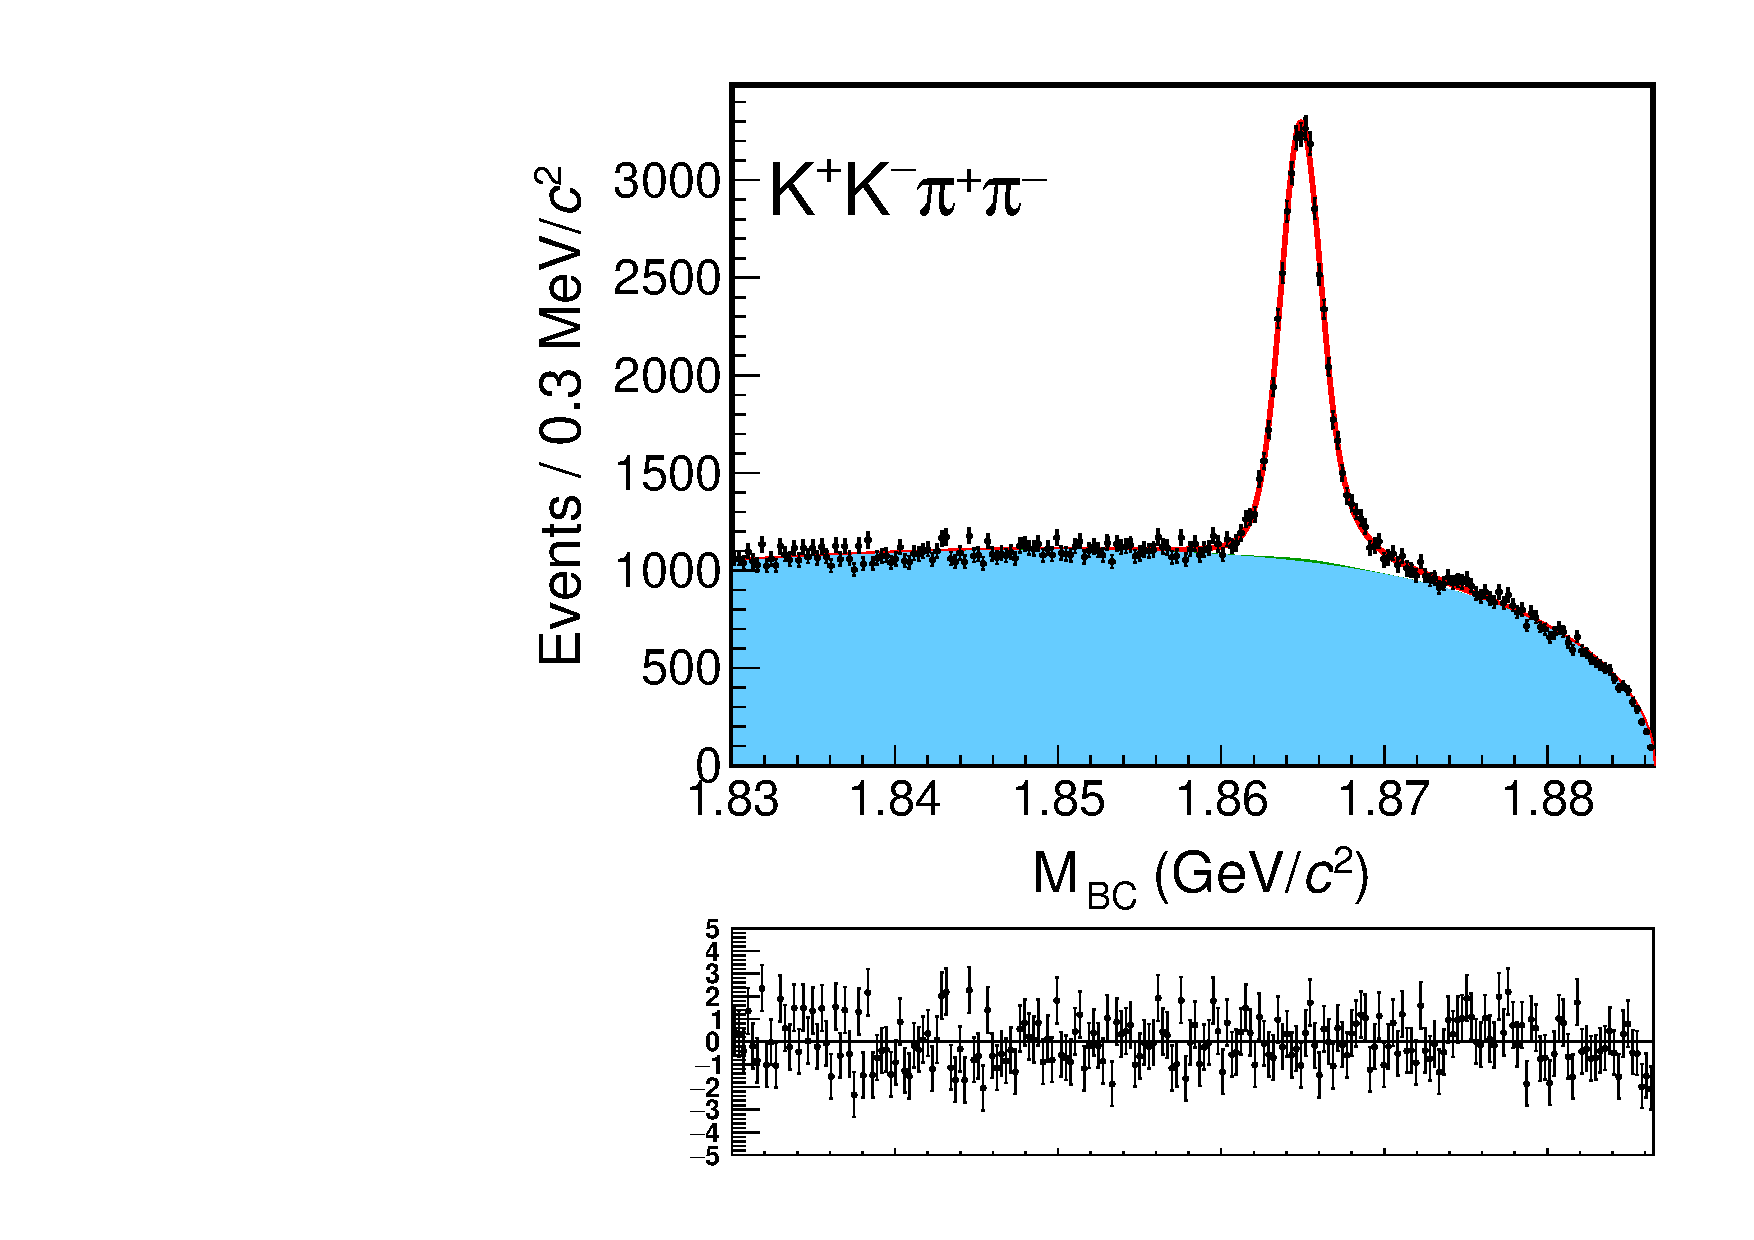
\includegraphics[height=3cm,trim={0 5.0cm 0 0},clip=true]{Plots/KKpipi_SingleTag_MBC_Plot.pdf}
      \caption{Single tag yield: $\SI{29227(268)}{}$}
    \end{subfigure}
  \end{figure}
\end{frame}

\section{Partially reconstructed \texorpdfstring{$D^0\to K^+K^-\pi^+\pi^-$}{D02KKpipi}}
\begin{frame}{Partially reconstructed $D^0\to K^+K^-\pi^+\pi^-$}
  \begin{itemize}
    \item{The reconstruction efficiency of $D\to KK\pi\pi$ is less than $20\%$}
    \item{For comparison, the efficiency of $D\to\pi\pi\pi\pi$ is around $50\%$!}
    \item{Poor kaon tracking efficiency at low momentum}
  \end{itemize}
  \begin{figure}
    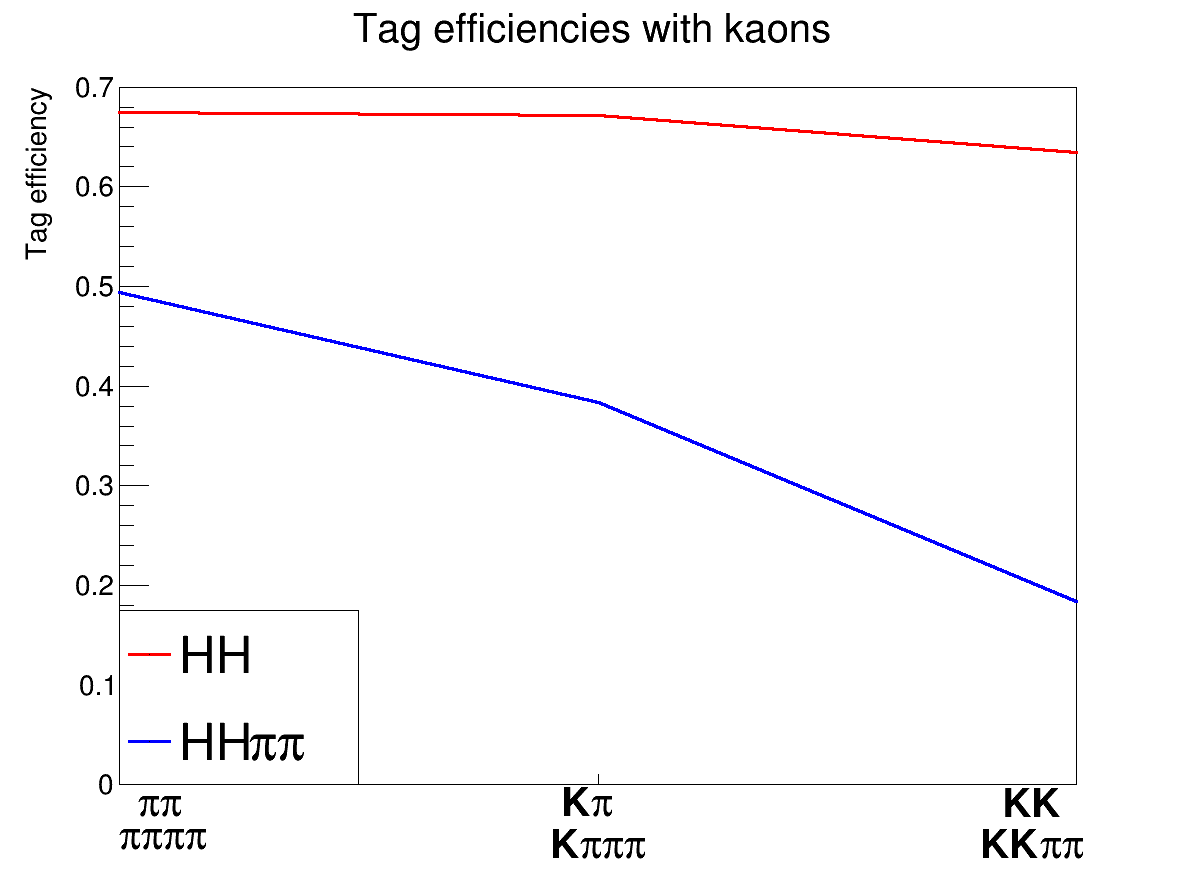
\includegraphics[width=0.6\textwidth]{Plots/KaonTrackingEfficiency.png}
  \end{figure}
\end{frame}

\begin{frame}{Partially reconstructed $D^0\to K^+K^-\pi^+\pi^-$}
  \begin{itemize}
    \item{Solution: Only reconstruct $3$ of the charged $D$ daughters}
    \begin{itemize}
      \item{Presence of missing kaon is inferred from the missing momentum}
      \item{Yields are similar to fully reconstructed sample}
      \item{Large, but non-peaking background from $D\to K\pi\pi\pi\pi^0$}
    \end{itemize}
  \end{itemize}
  \begin{figure}[H]
    \centering
    \vspace{0.3cm}
    \begin{fmffile}{fgraph/fgraph_PartRecoKKpipi}
      \setlength{\unitlength}{1cm}
      \begin{fmfgraph*}(8,4)
        \fmfstraight
        \fmfleft{i4,i3,i2,i1}
        \fmfright{g1,o1,o2,g2}
        \fmflabel{$K^+$}{o1}
        \fmflabel{$K^-$}{o2}
        \fmflabel{$K^+$}{i1}
        \fmflabel{$K^-$}{i2}
        \fmflabel{$\pi^+$}{i3}
        \fmflabel{$\pi^-$}{i4}
        \fmf{dashes}{w,i1}
        \fmf{plain}{w,i2}
        \fmf{plain}{w,i3}
        \fmf{plain}{w,i4}
        \fmf{plain}{w,o1}
        \fmf{plain}{w,o2}
        \fmf{phantom}{w,g1}
        \fmf{phantom}{w,g2}
        \fmfblob{1cm}{w}
      \end{fmfgraph*}
    \end{fmffile}
    \vspace{0.3cm}
  \end{figure}
  \begin{center}
    Use this technique with the $K^+K^-$, $K_S^0\pi^0$ and $K_S^0\pi^+\pi^-$ tags
  \end{center}
\end{frame}

\section{Fit of double tag yields}
\begin{frame}{Double tag fits}
  \begin{itemize}
    \setlength\itemsep{1.0em}
    \item{Fit strategy: Only fit signal side $m_{\rm BC}$ because of low statistics}
    \item{Fit model:}
    \begin{itemize}
      \item{Signal: PDF from signal MC, convolved with a Gaussian}
      \item{Flatackground: Argus PDF}
      \item{Peaking background: Shape and efficiency from MC, correct for quantum correlation}
      \item{Simple sideband subtraction for correct signal but wrong tag event}
    \end{itemize}
    \item{Fit all bins simultaneously}
    \begin{itemize}
      \item{Shape is floated and shared across all bins}
      \item{Yield of signal and combinatorial background is floated in each bin}
    \end{itemize}
  \end{itemize}
\end{frame}

\begin{frame}{Double tag fit of $KK\pi\pi$ vs $K\pi$}
  \begin{figure}
    \centering
    \begin{subfigure}{0.5\textwidth}
      \centering
      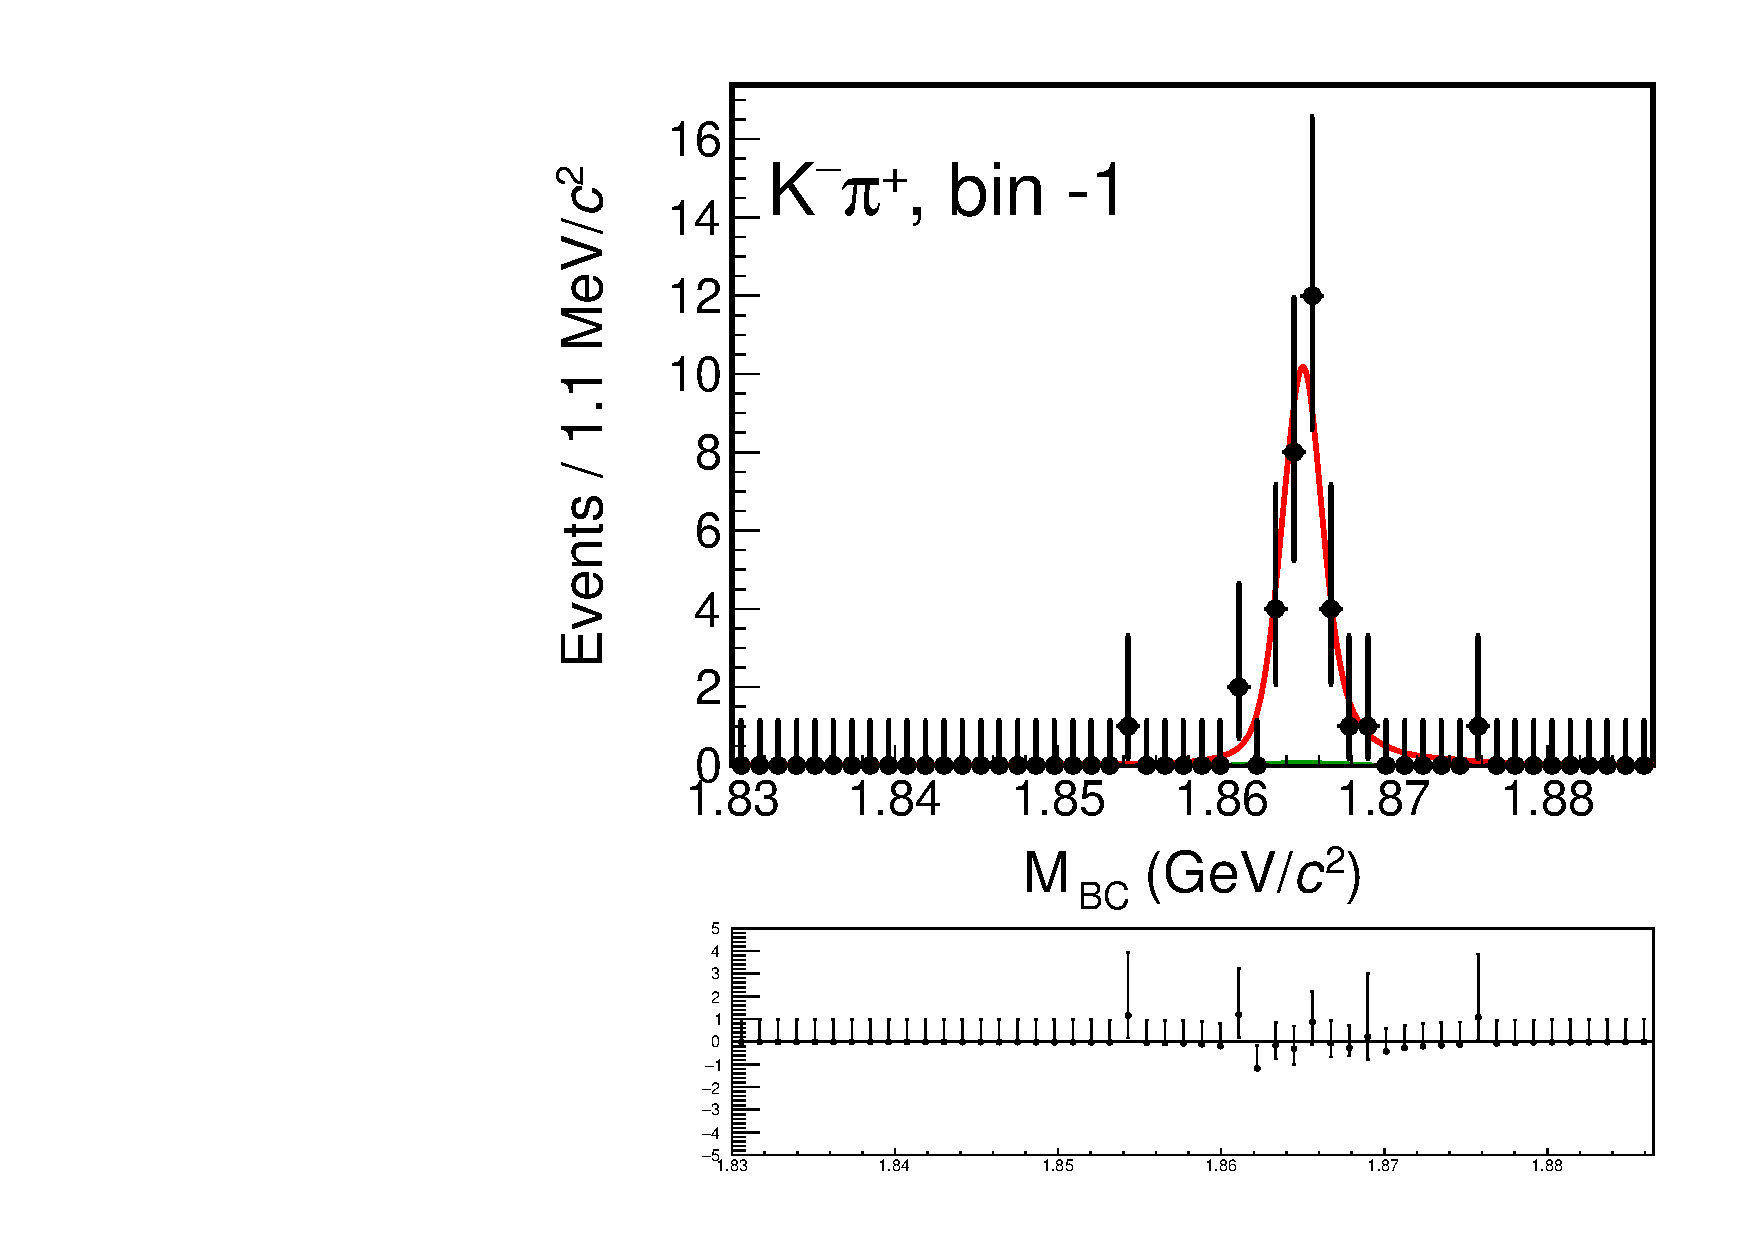
\includegraphics[width=0.75\textwidth,trim={0 5cm 0 0},clip=true]{Plots/DoubleTagYield_DoubleTag_Flavour_KKpipi_vs_Kpi_SignalBinM1_TagBin0.pdf}
      \caption{Bin $-1$ yield: $32.4_{-5.5}^{+6.2}$}
    \end{subfigure}%
    \begin{subfigure}{0.5\textwidth}
      \centering
      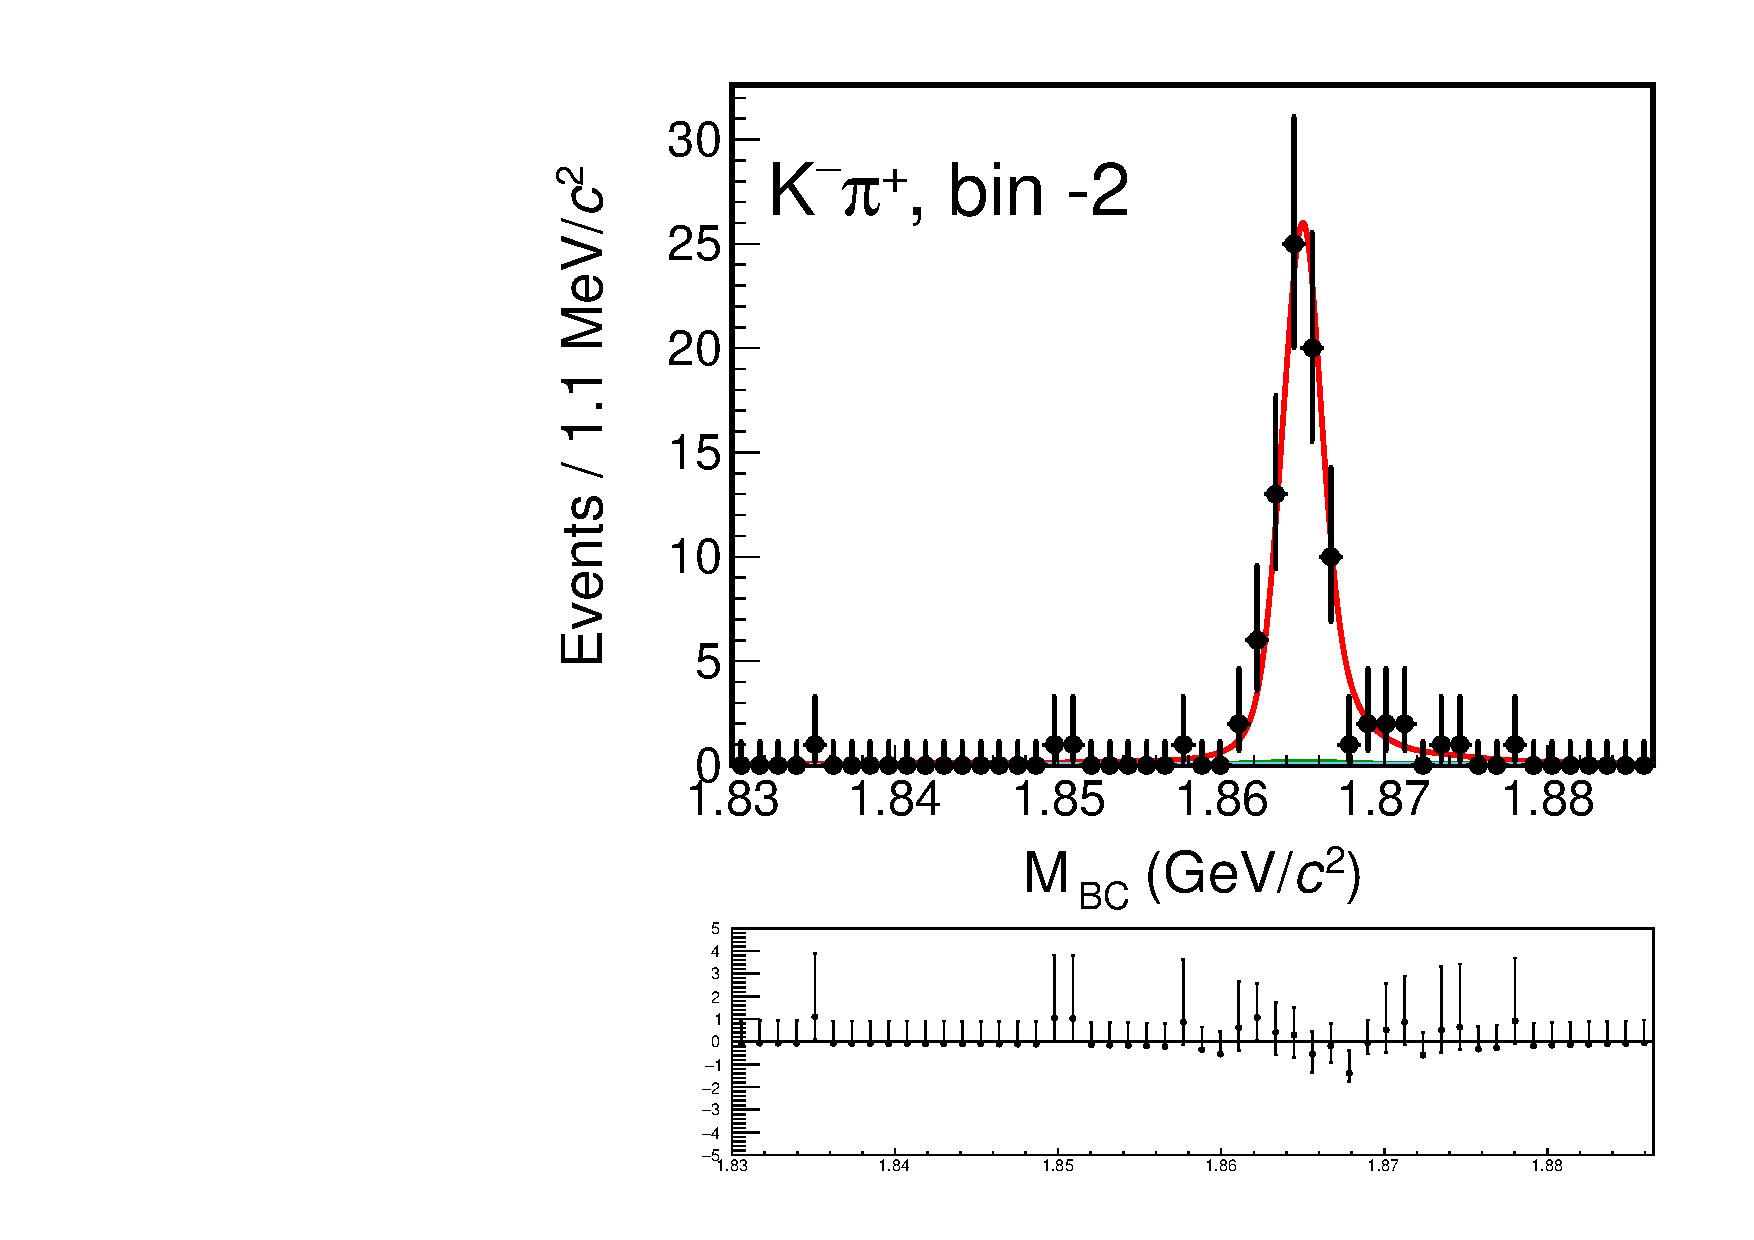
\includegraphics[width=0.75\textwidth,trim={0 5cm 0 0},clip=true]{Plots/DoubleTagYield_DoubleTag_Flavour_KKpipi_vs_Kpi_SignalBinM2_TagBin0.pdf}
      \caption{Bin $-2$ yield: $82.7_{-9.0}^{+9.7}$}
    \end{subfigure}
    \begin{subfigure}{0.5\textwidth}
      \centering
      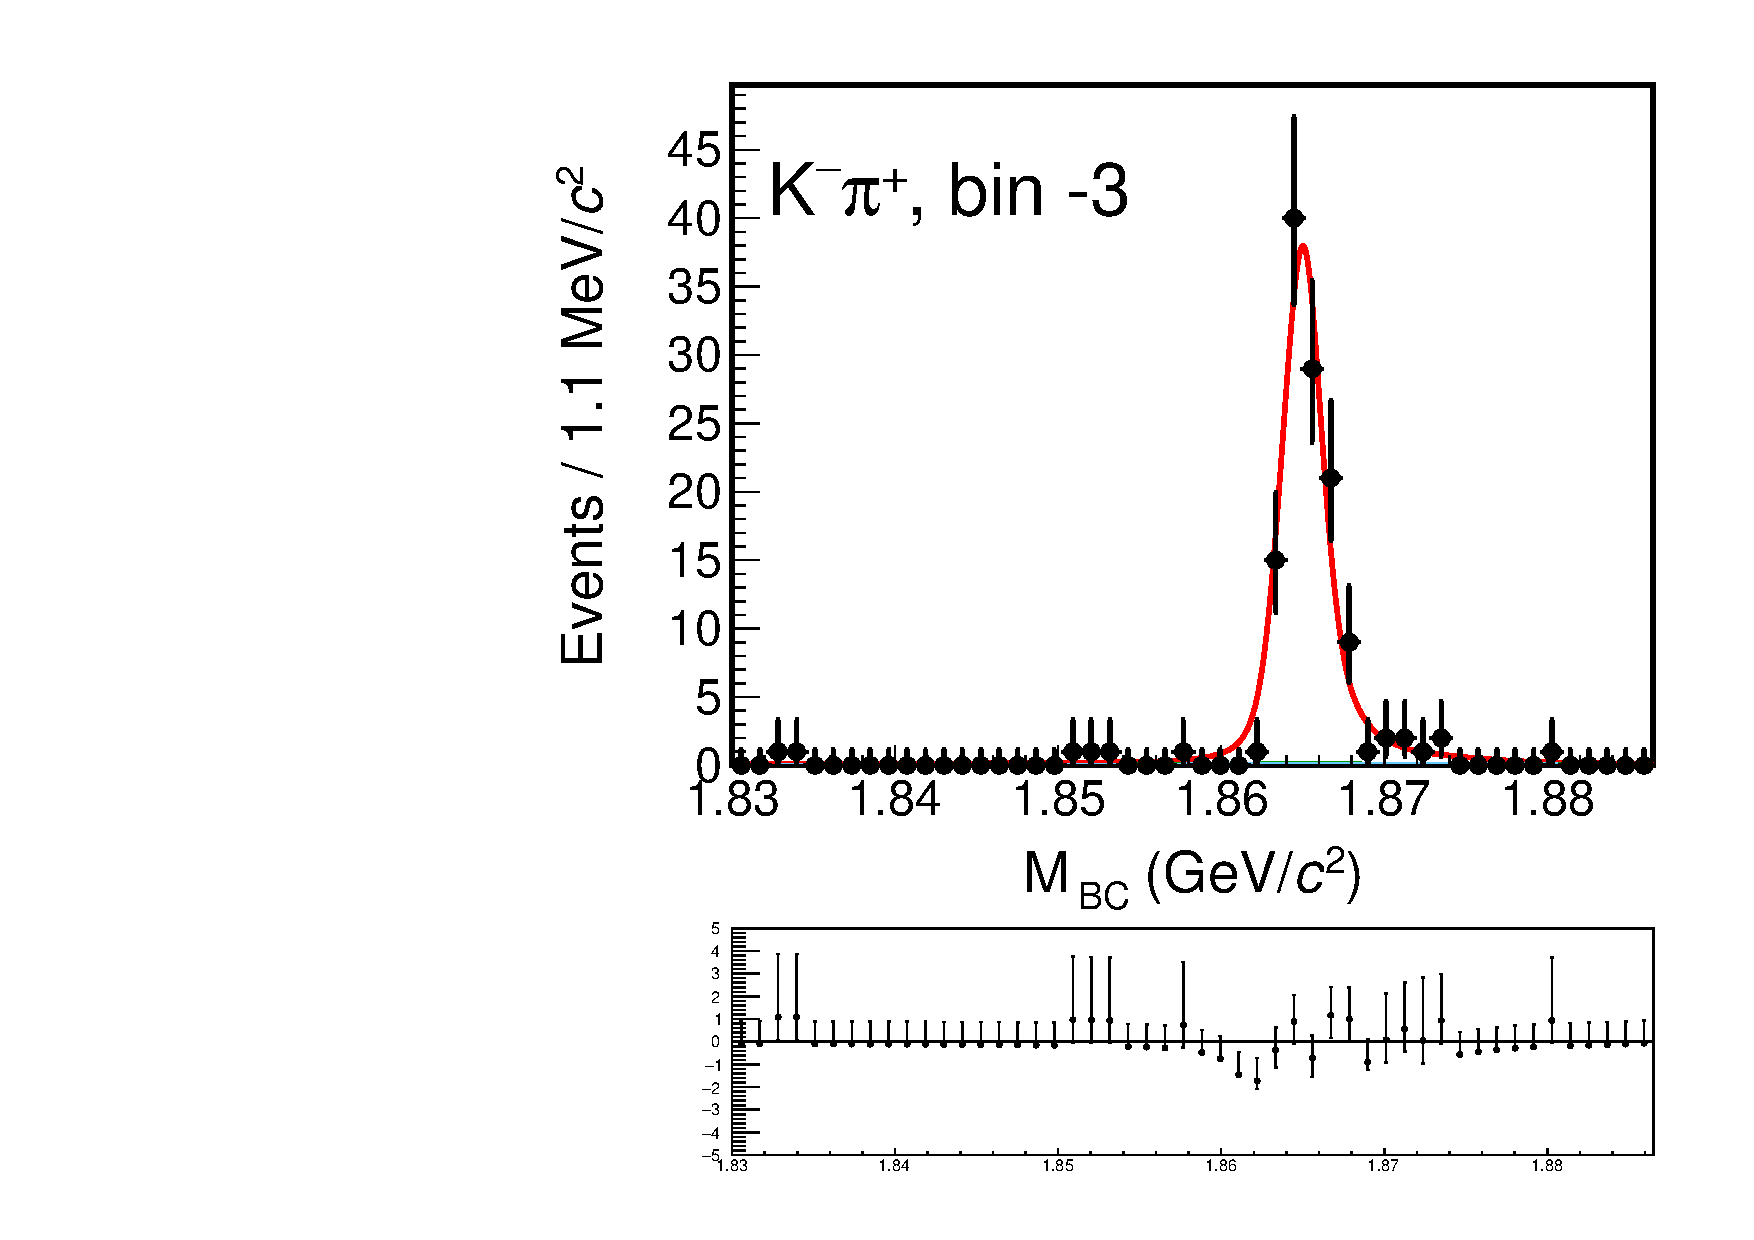
\includegraphics[width=0.75\textwidth,trim={0 5cm 0 0},clip=true]{Plots/DoubleTagYield_DoubleTag_Flavour_KKpipi_vs_Kpi_SignalBinM3_TagBin0.pdf}
      \caption{Bin $-3$ yield: $120.3_{-10.9}^{+11.6}$}
    \end{subfigure}%
    \begin{subfigure}{0.5\textwidth}
      \centering
      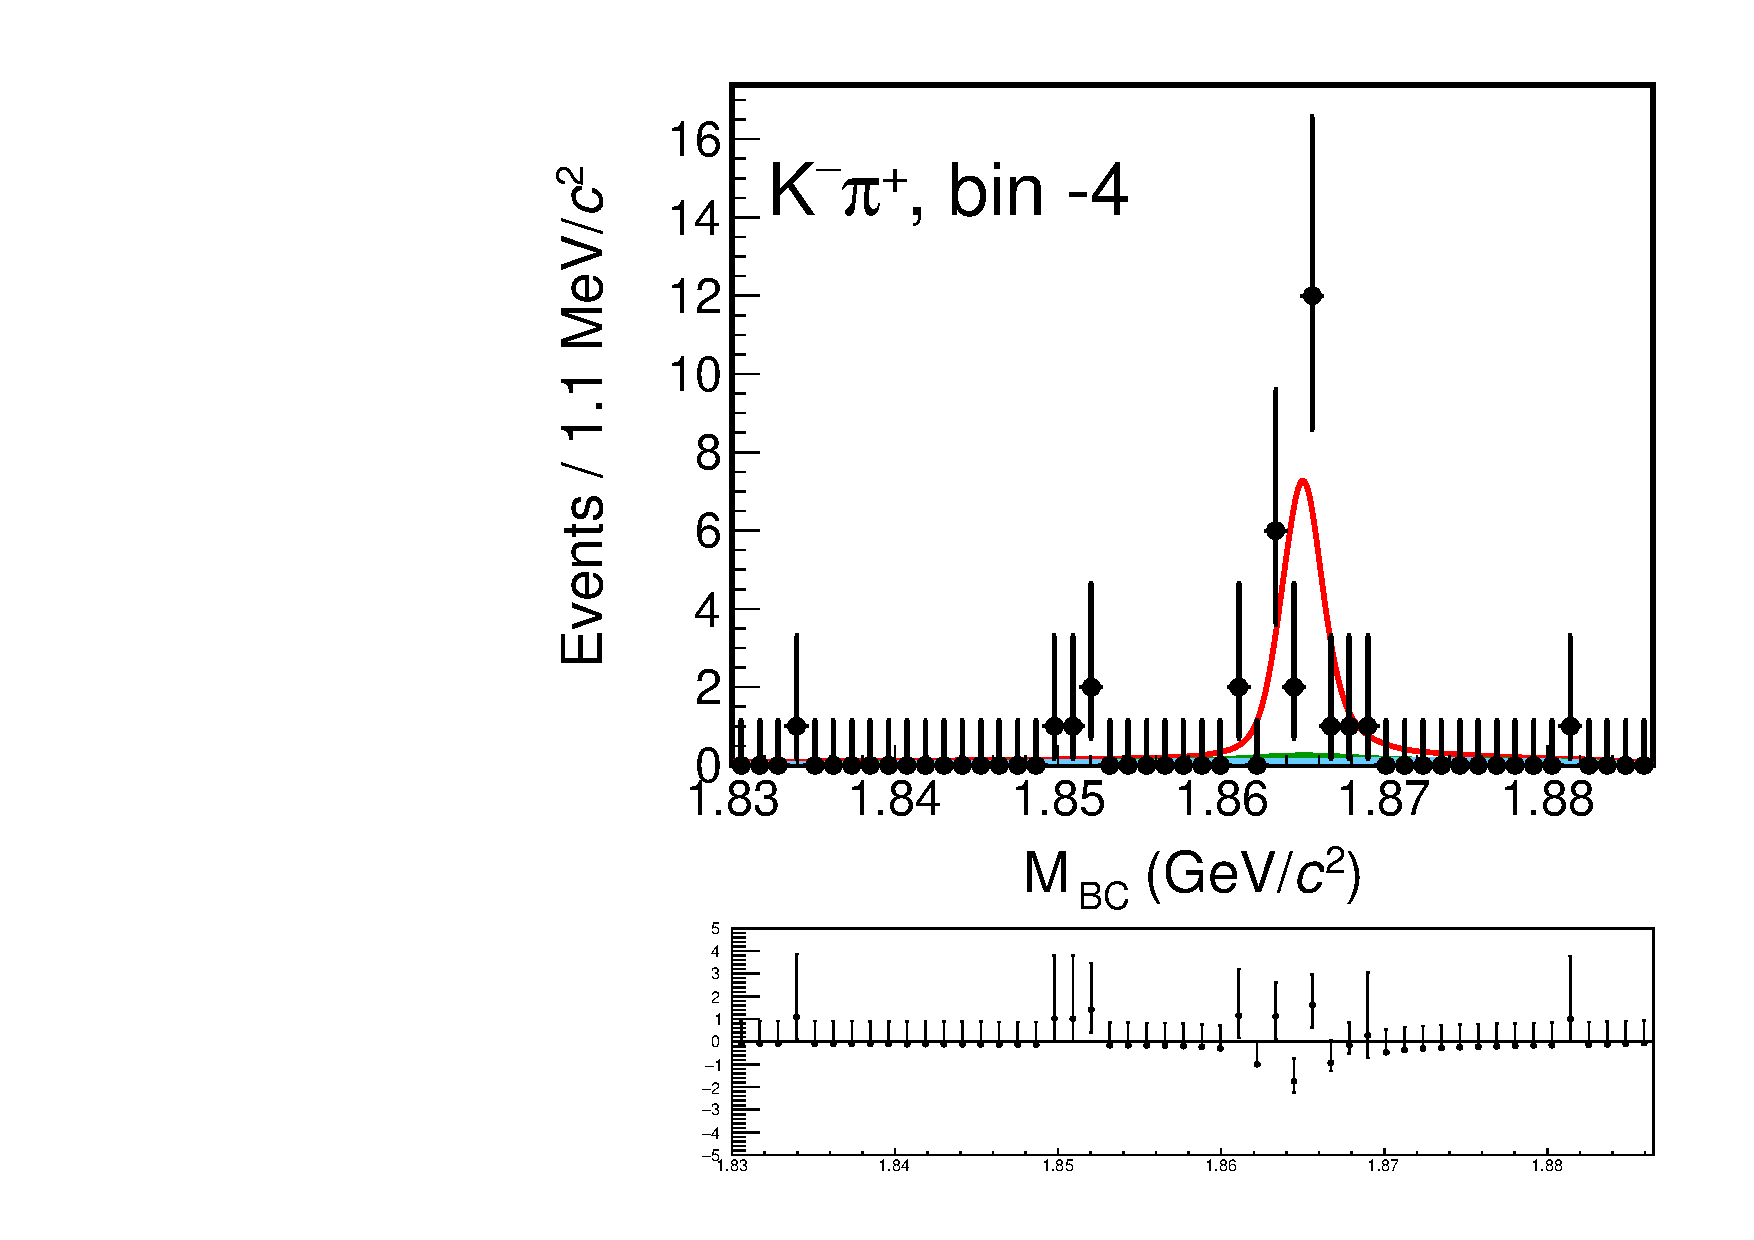
\includegraphics[width=0.75\textwidth,trim={0 5cm 0 0},clip=true]{Plots/DoubleTagYield_DoubleTag_Flavour_KKpipi_vs_Kpi_SignalBinM4_TagBin0.pdf}
      \caption{Bin $-4$ yield: $22.4_{-4.6}^{+5.2}$}
    \end{subfigure}
  \end{figure}
\end{frame}

\begin{frame}{Double tag fit of $KK\pi\pi$ vs $K\pi$}
  \begin{figure}
    \centering
    \begin{subfigure}{0.5\textwidth}
      \centering
      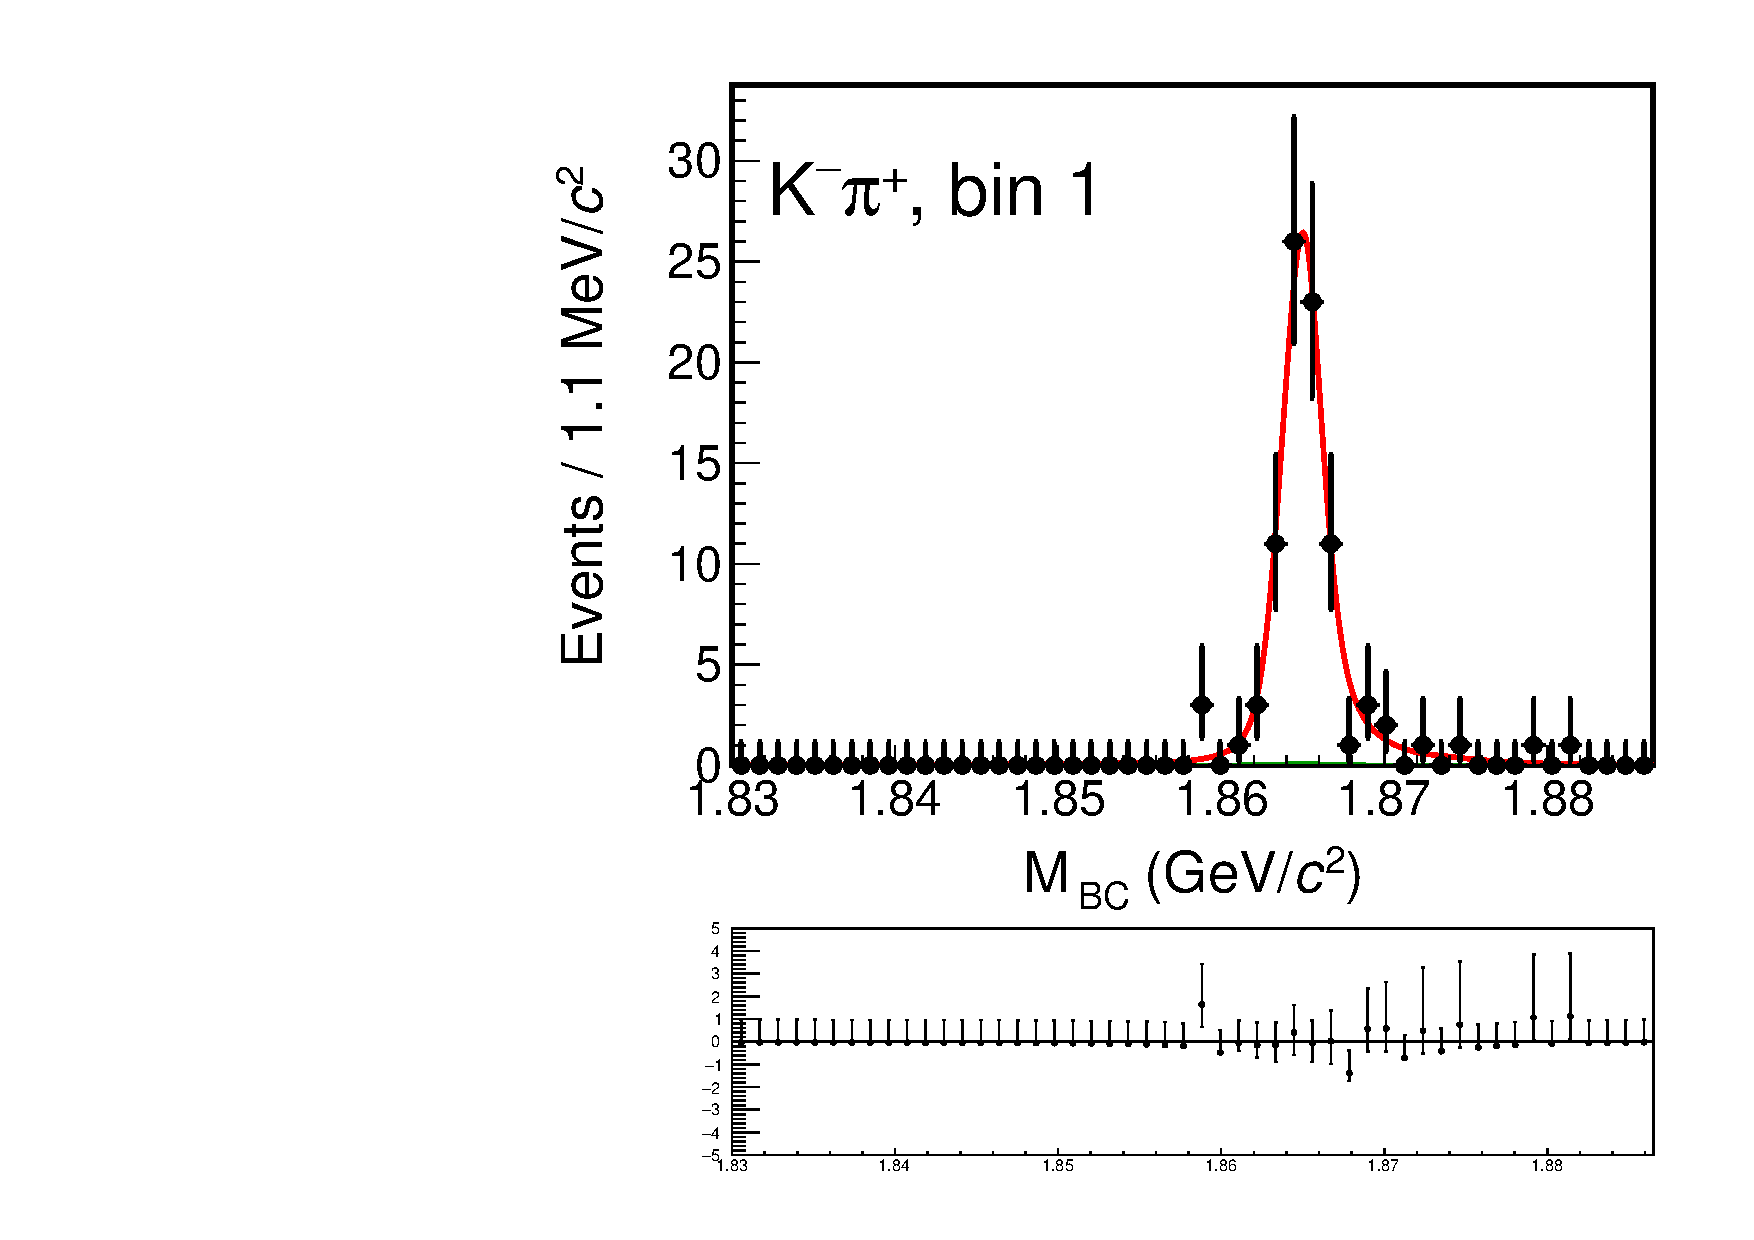
\includegraphics[width=0.75\textwidth,trim={0 5cm 0 0},clip=true]{Plots/DoubleTagYield_DoubleTag_Flavour_KKpipi_vs_Kpi_SignalBinP1_TagBin0.pdf}
      \caption{Bin $1$ yield: $84.5_{-9.1}^{+9.8}$}
    \end{subfigure}%
    \begin{subfigure}{0.5\textwidth}
      \centering
      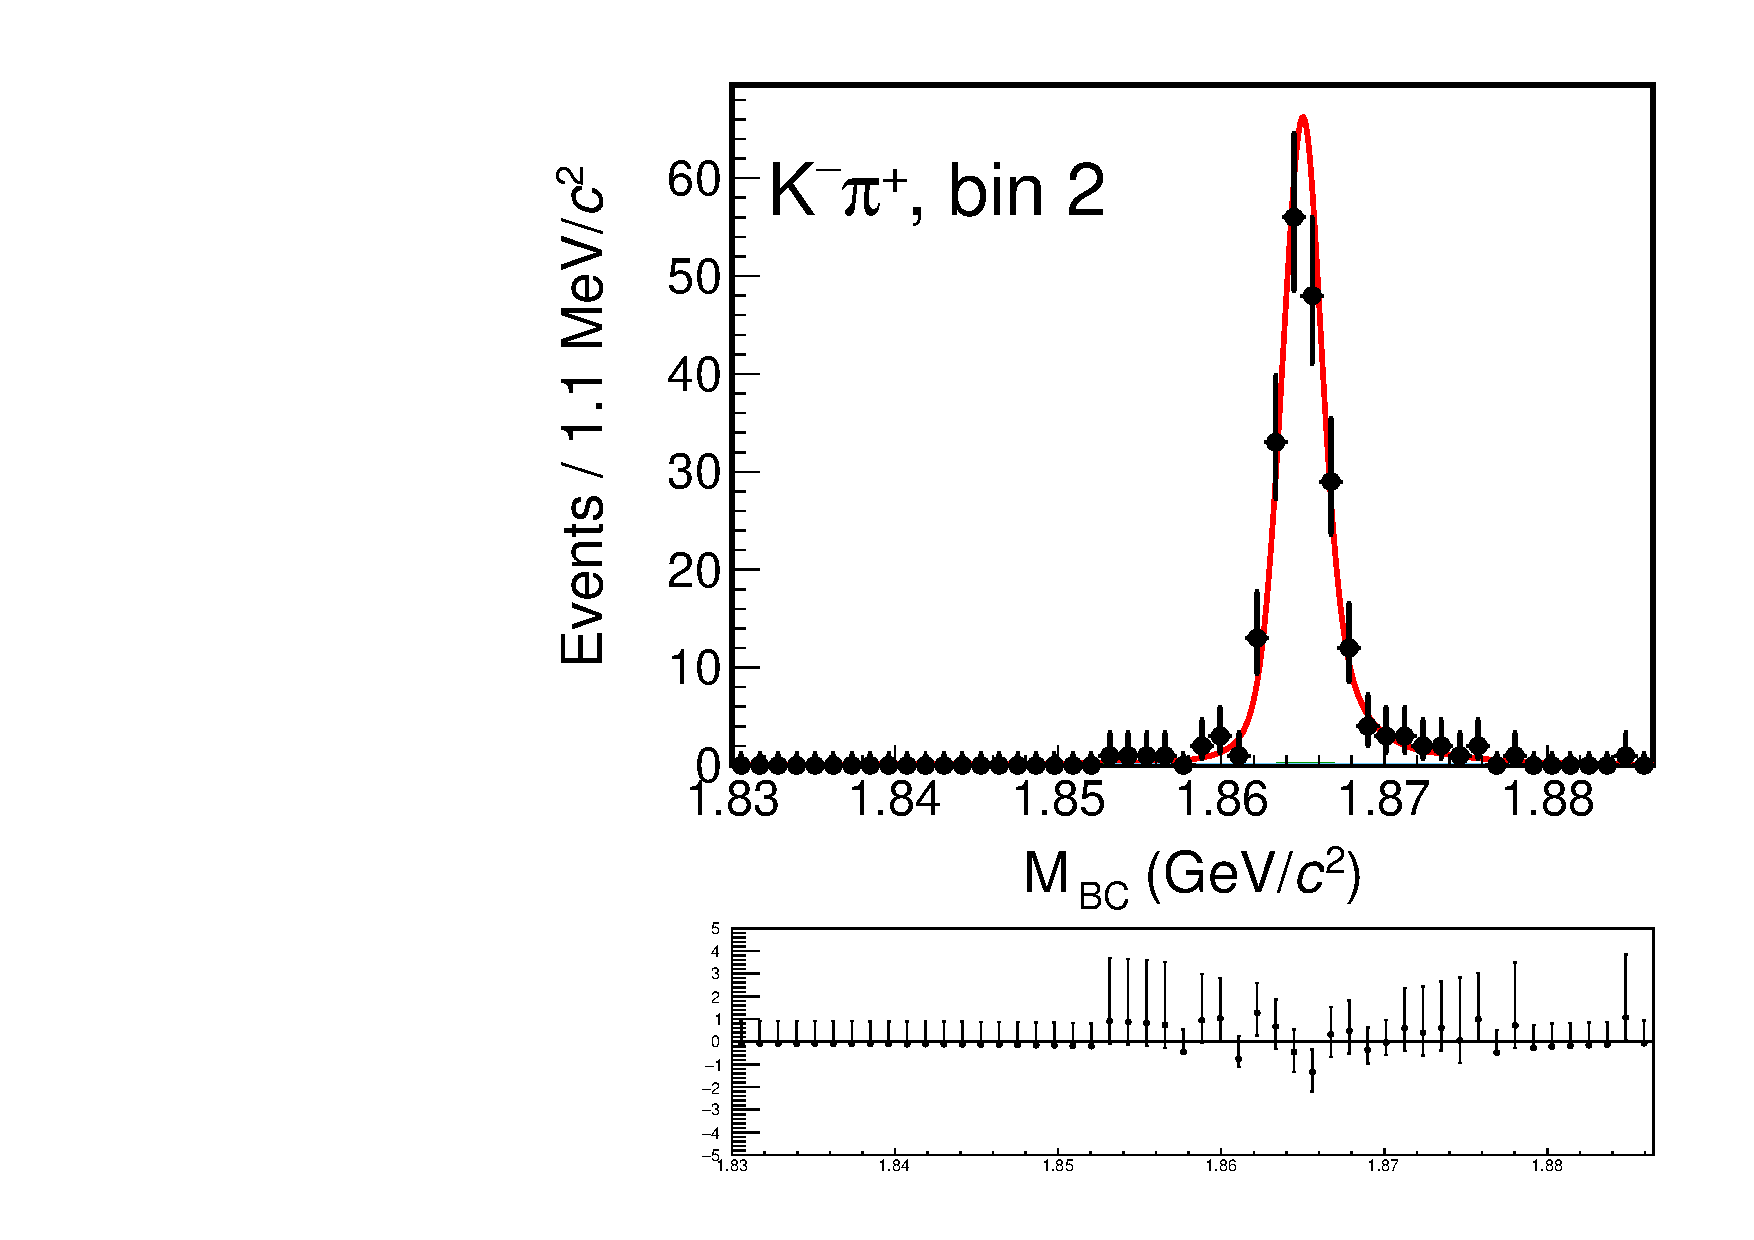
\includegraphics[width=0.75\textwidth,trim={0 5cm 0 0},clip=true]{Plots/DoubleTagYield_DoubleTag_Flavour_KKpipi_vs_Kpi_SignalBinP2_TagBin0.pdf}
      \caption{Bin $2$ yield: $211.2_{-14.8}^{+15.4}$}
    \end{subfigure}
    \begin{subfigure}{0.5\textwidth}
      \centering
      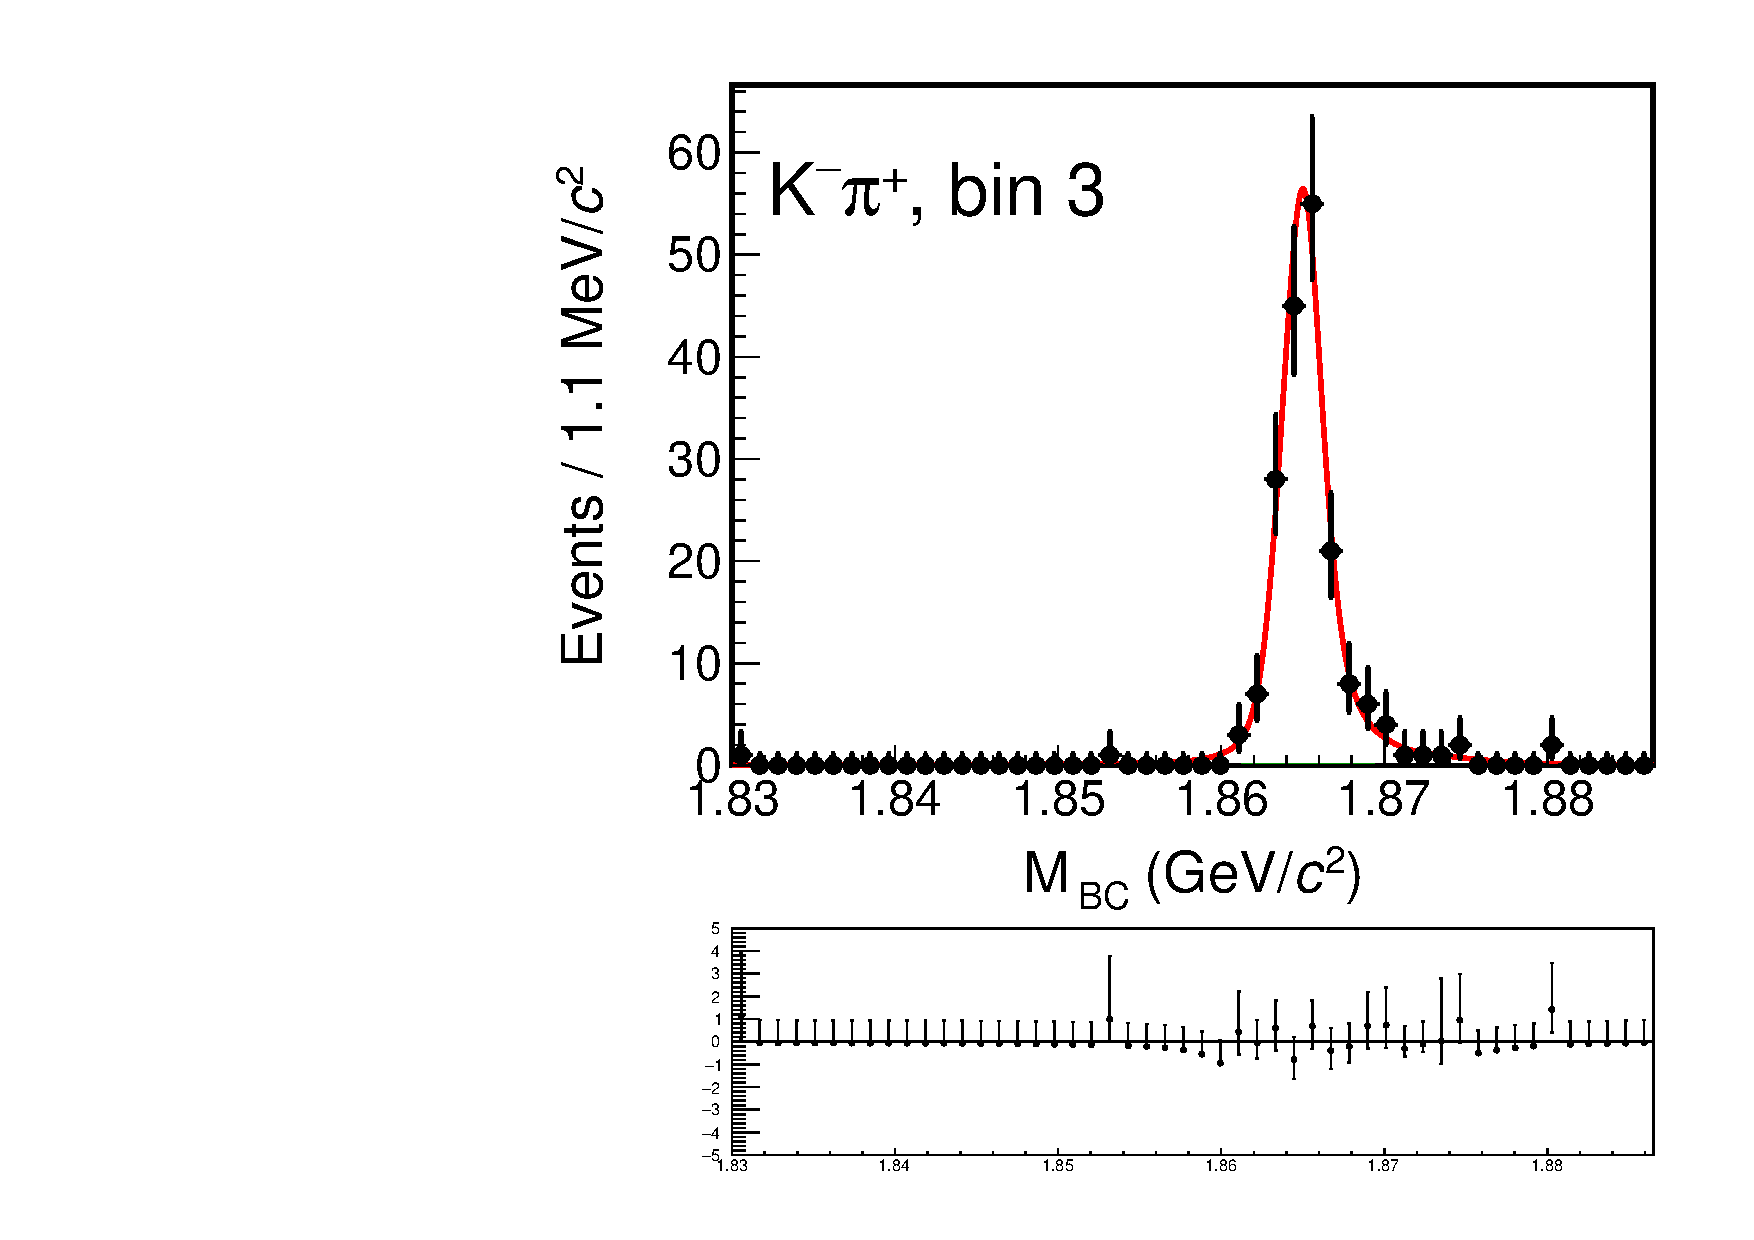
\includegraphics[width=0.75\textwidth,trim={0 5cm 0 0},clip=true]{Plots/DoubleTagYield_DoubleTag_Flavour_KKpipi_vs_Kpi_SignalBinP3_TagBin0.pdf}
      \caption{Bin $3$ yield: $181.0_{-13.3}^{+14.0}$}
    \end{subfigure}%
    \begin{subfigure}{0.5\textwidth}
      \centering
      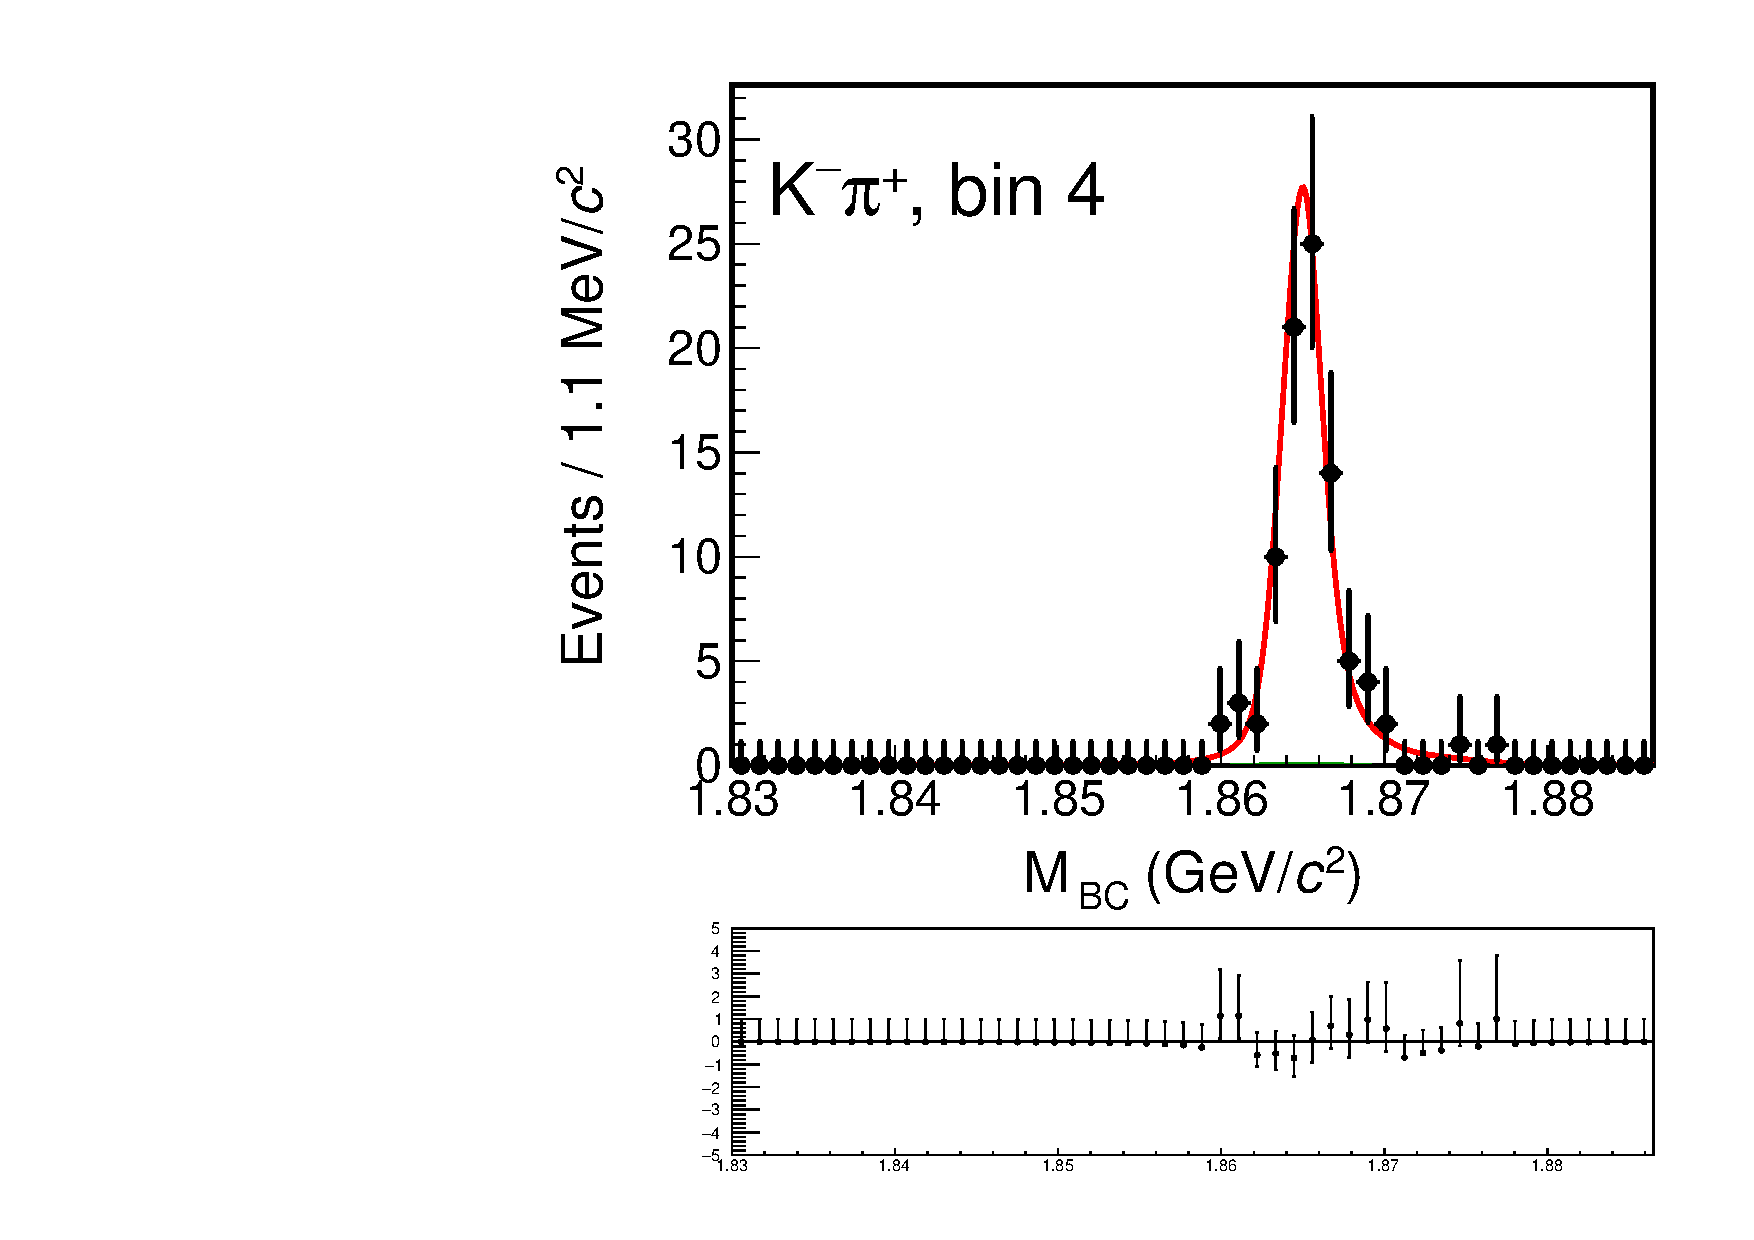
\includegraphics[width=0.75\textwidth,trim={0 5cm 0 0},clip=true]{Plots/DoubleTagYield_DoubleTag_Flavour_KKpipi_vs_Kpi_SignalBinP4_TagBin0.pdf}
      \caption{Bin $4$ yield: $88.6_{-9.0}^{+9.7}$}
    \end{subfigure}
  \end{figure}
\end{frame}

\begin{frame}{Double tag fit of $KK\pi\pi$ vs $KK$}
  \begin{figure}
    \centering
    \begin{subfigure}{0.5\textwidth}
      \centering
      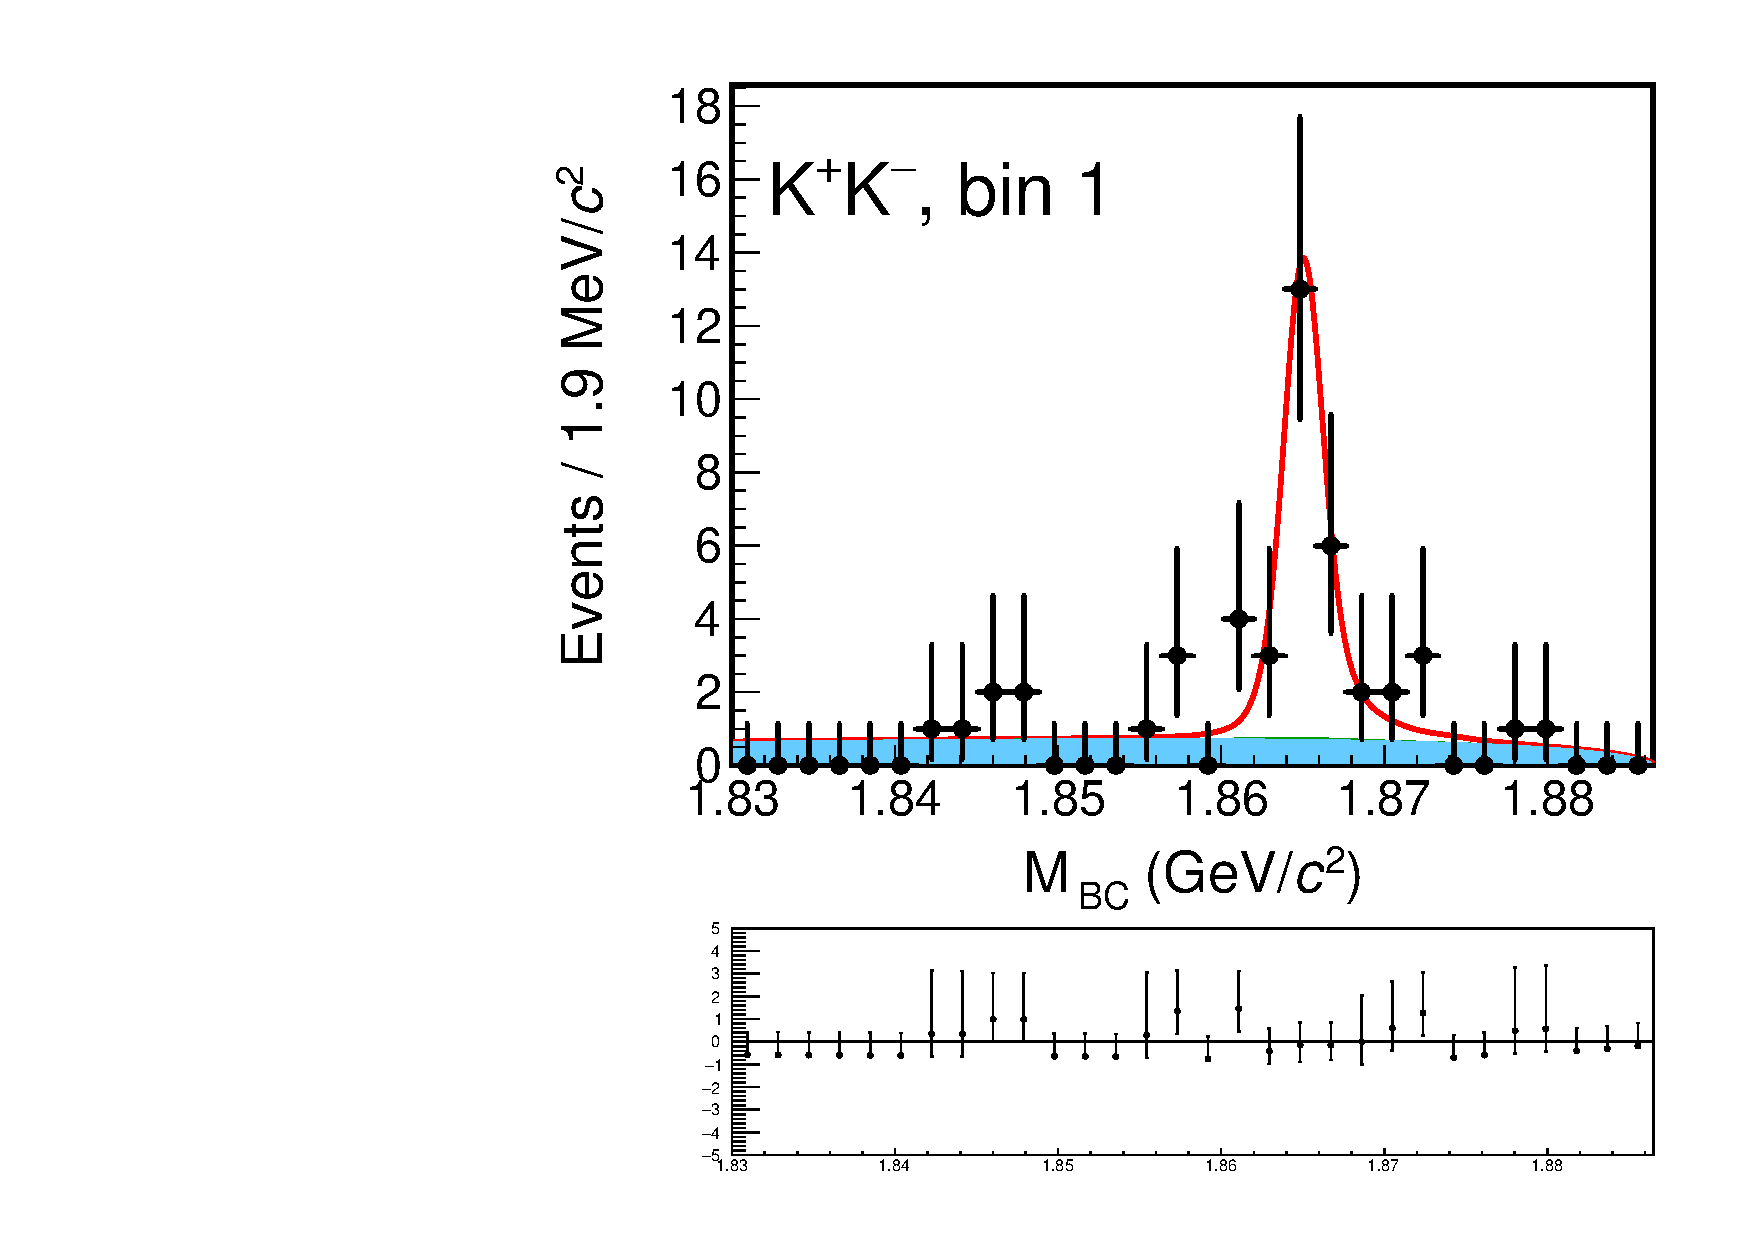
\includegraphics[width=0.75\textwidth,trim={0 5cm 0 0},clip=true]{Plots/DoubleTagYield_DoubleTag_CP_KKpipi_vs_KK_SignalBin1.pdf}
      \caption{Bin $1$ yield: $25.3_{-5.5}^{+6.2}$}
    \end{subfigure}%
    \begin{subfigure}{0.5\textwidth}
      \centering
      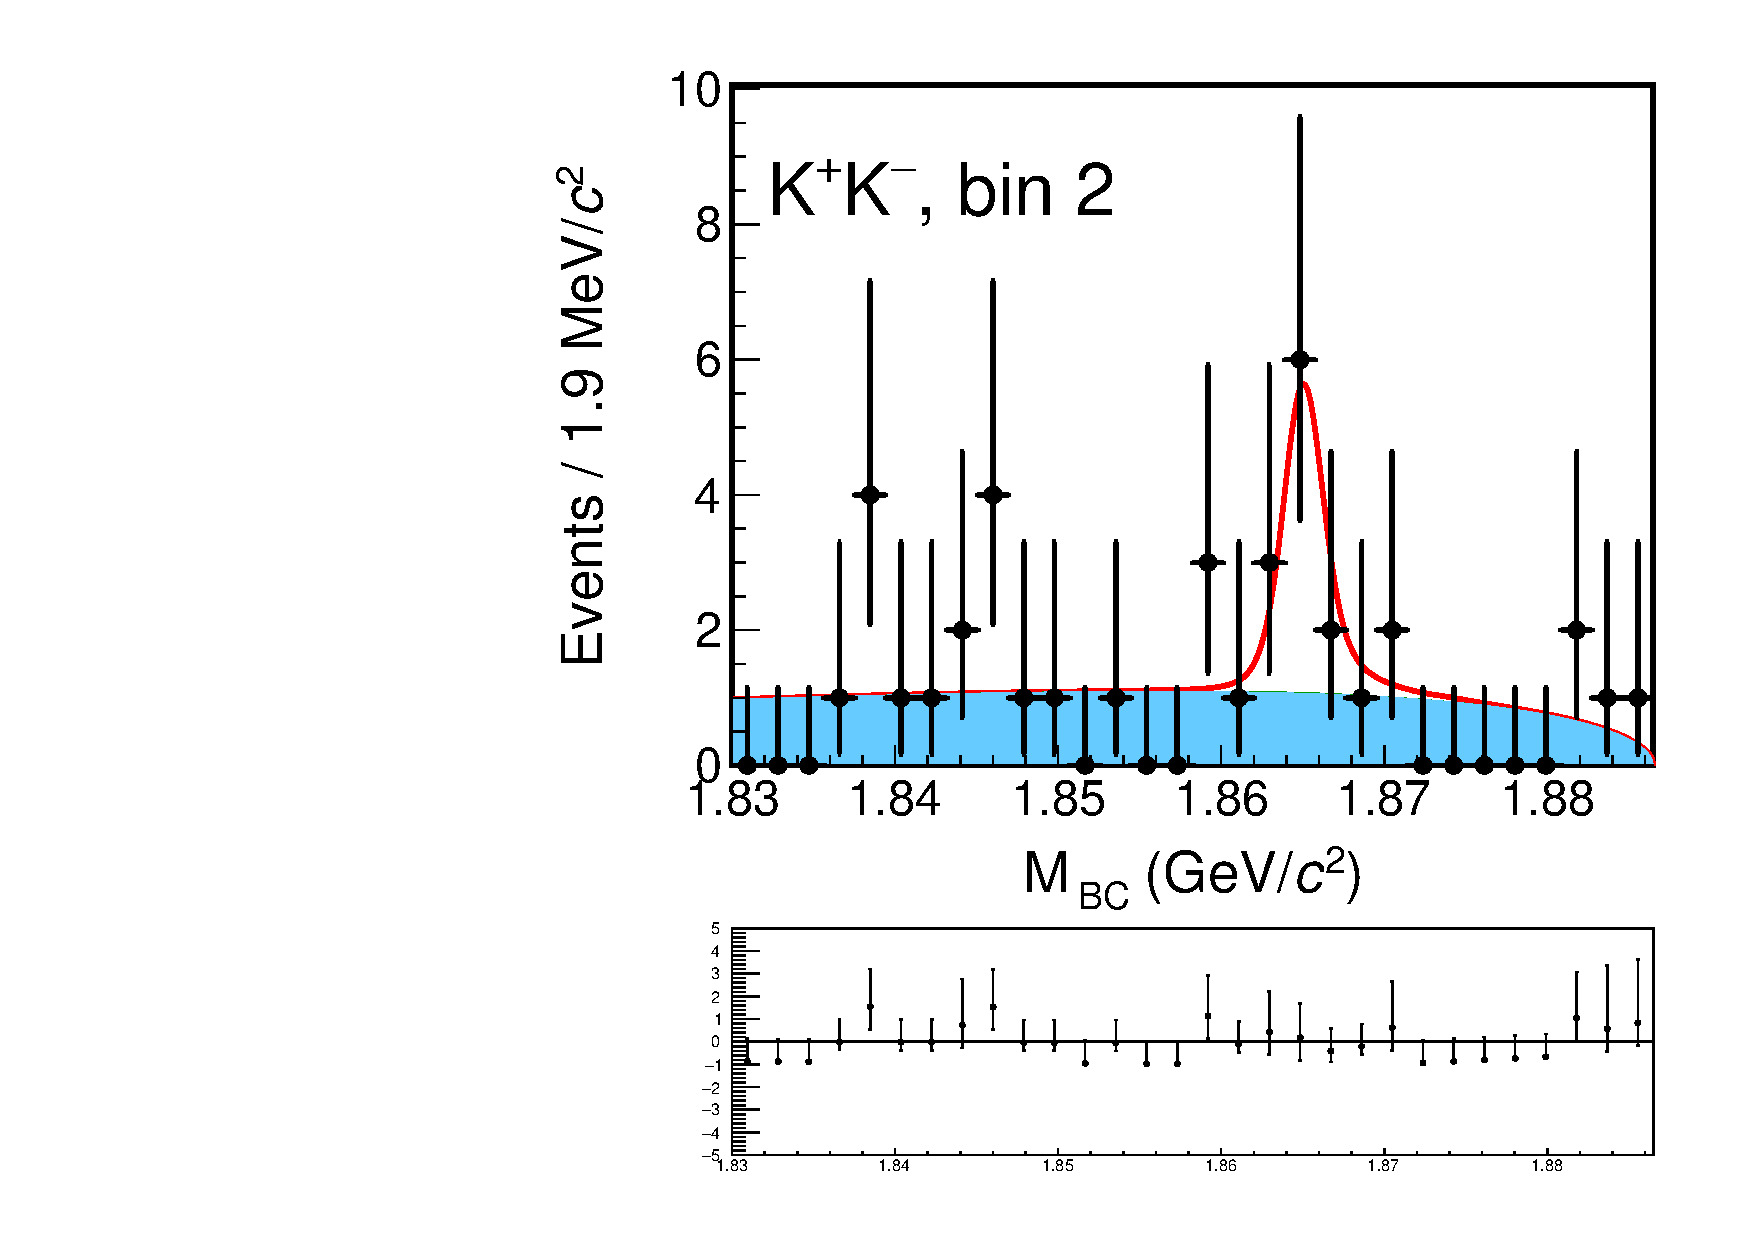
\includegraphics[width=0.75\textwidth,trim={0 5cm 0 0},clip=true]{Plots/DoubleTagYield_DoubleTag_CP_KKpipi_vs_KK_SignalBin2.pdf}
      \caption{Bin $2$ yield: $8.8_{-3.3}^{+4.0}$}
    \end{subfigure}
    \begin{subfigure}{0.5\textwidth}
      \centering
      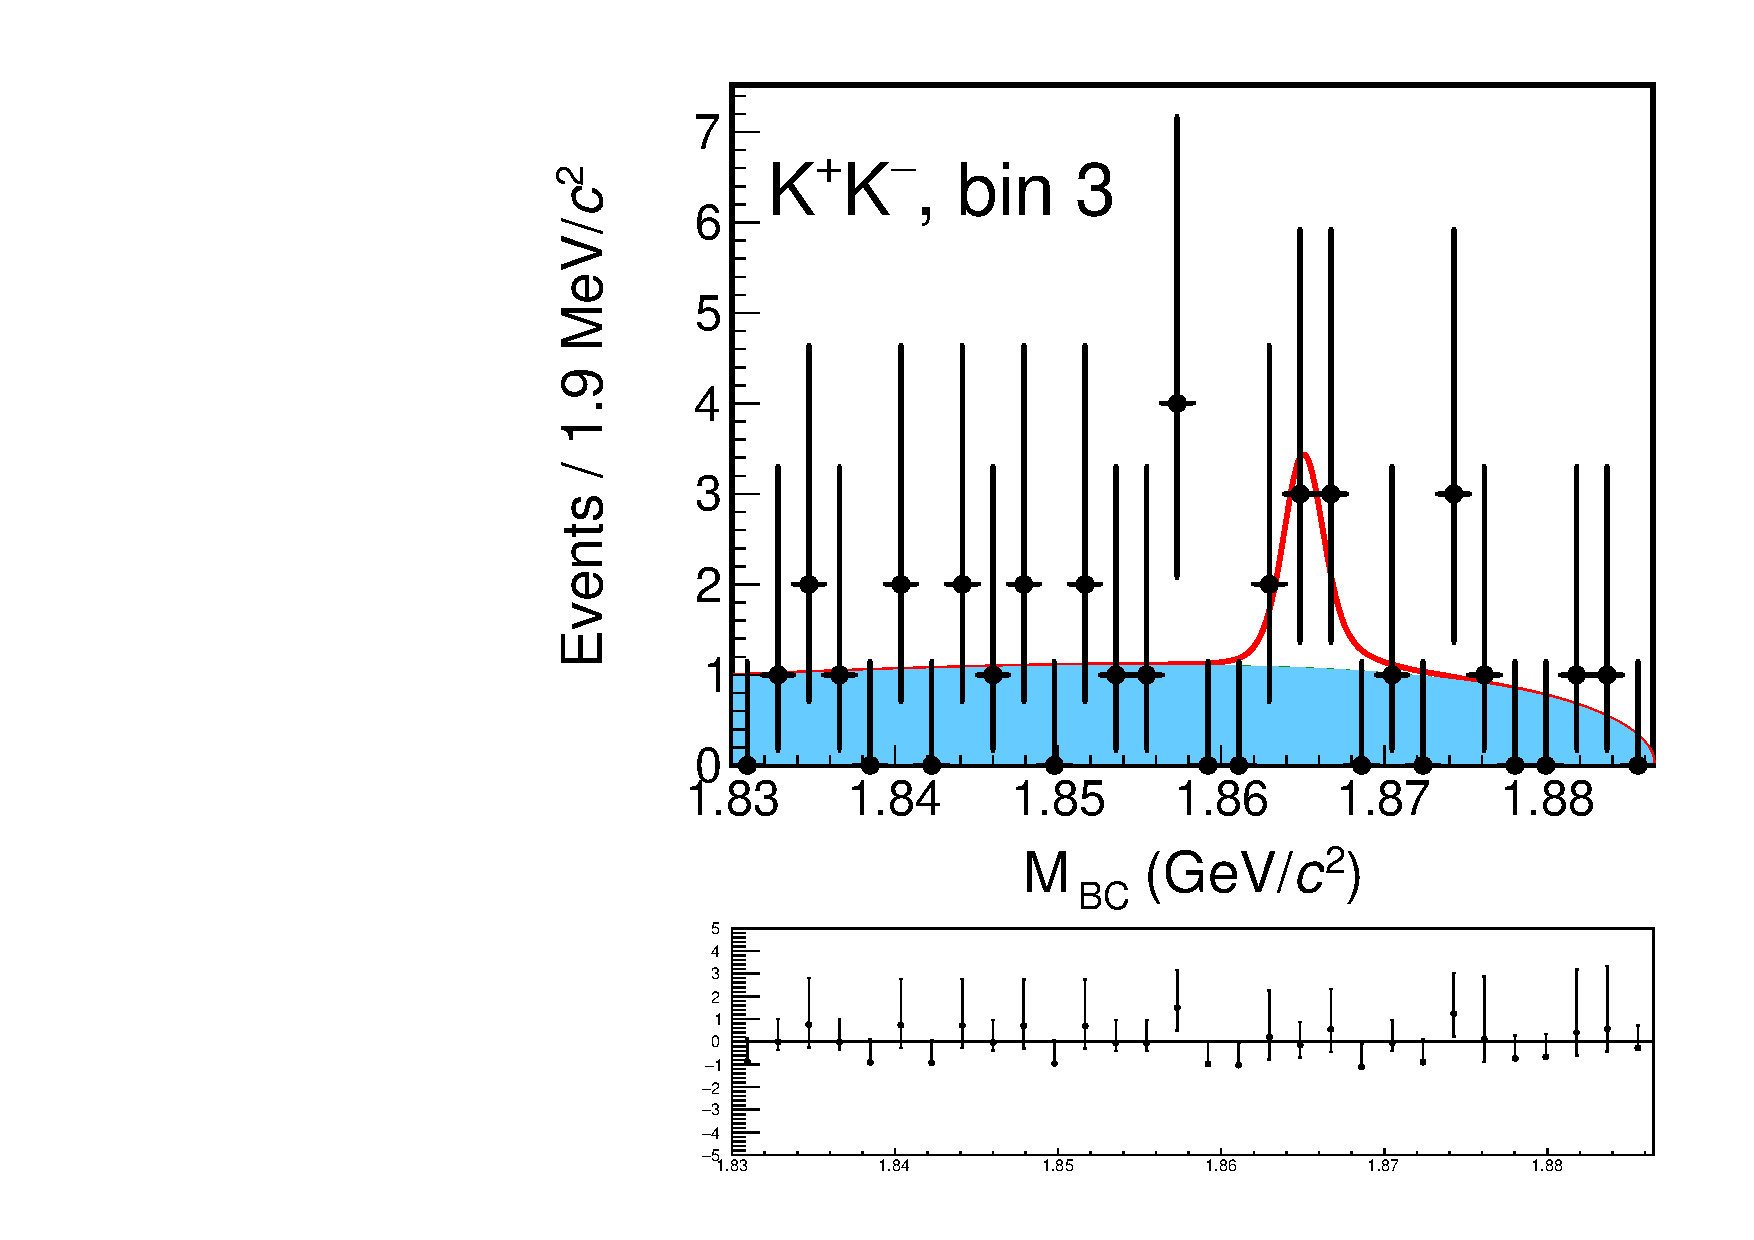
\includegraphics[width=0.75\textwidth,trim={0 5cm 0 0},clip=true]{Plots/DoubleTagYield_DoubleTag_CP_KKpipi_vs_KK_SignalBin3.pdf}
      \caption{Bin $3$ yield: $4.5_{-2.6}^{+3.3}$}
    \end{subfigure}%
    \begin{subfigure}{0.5\textwidth}
      \centering
      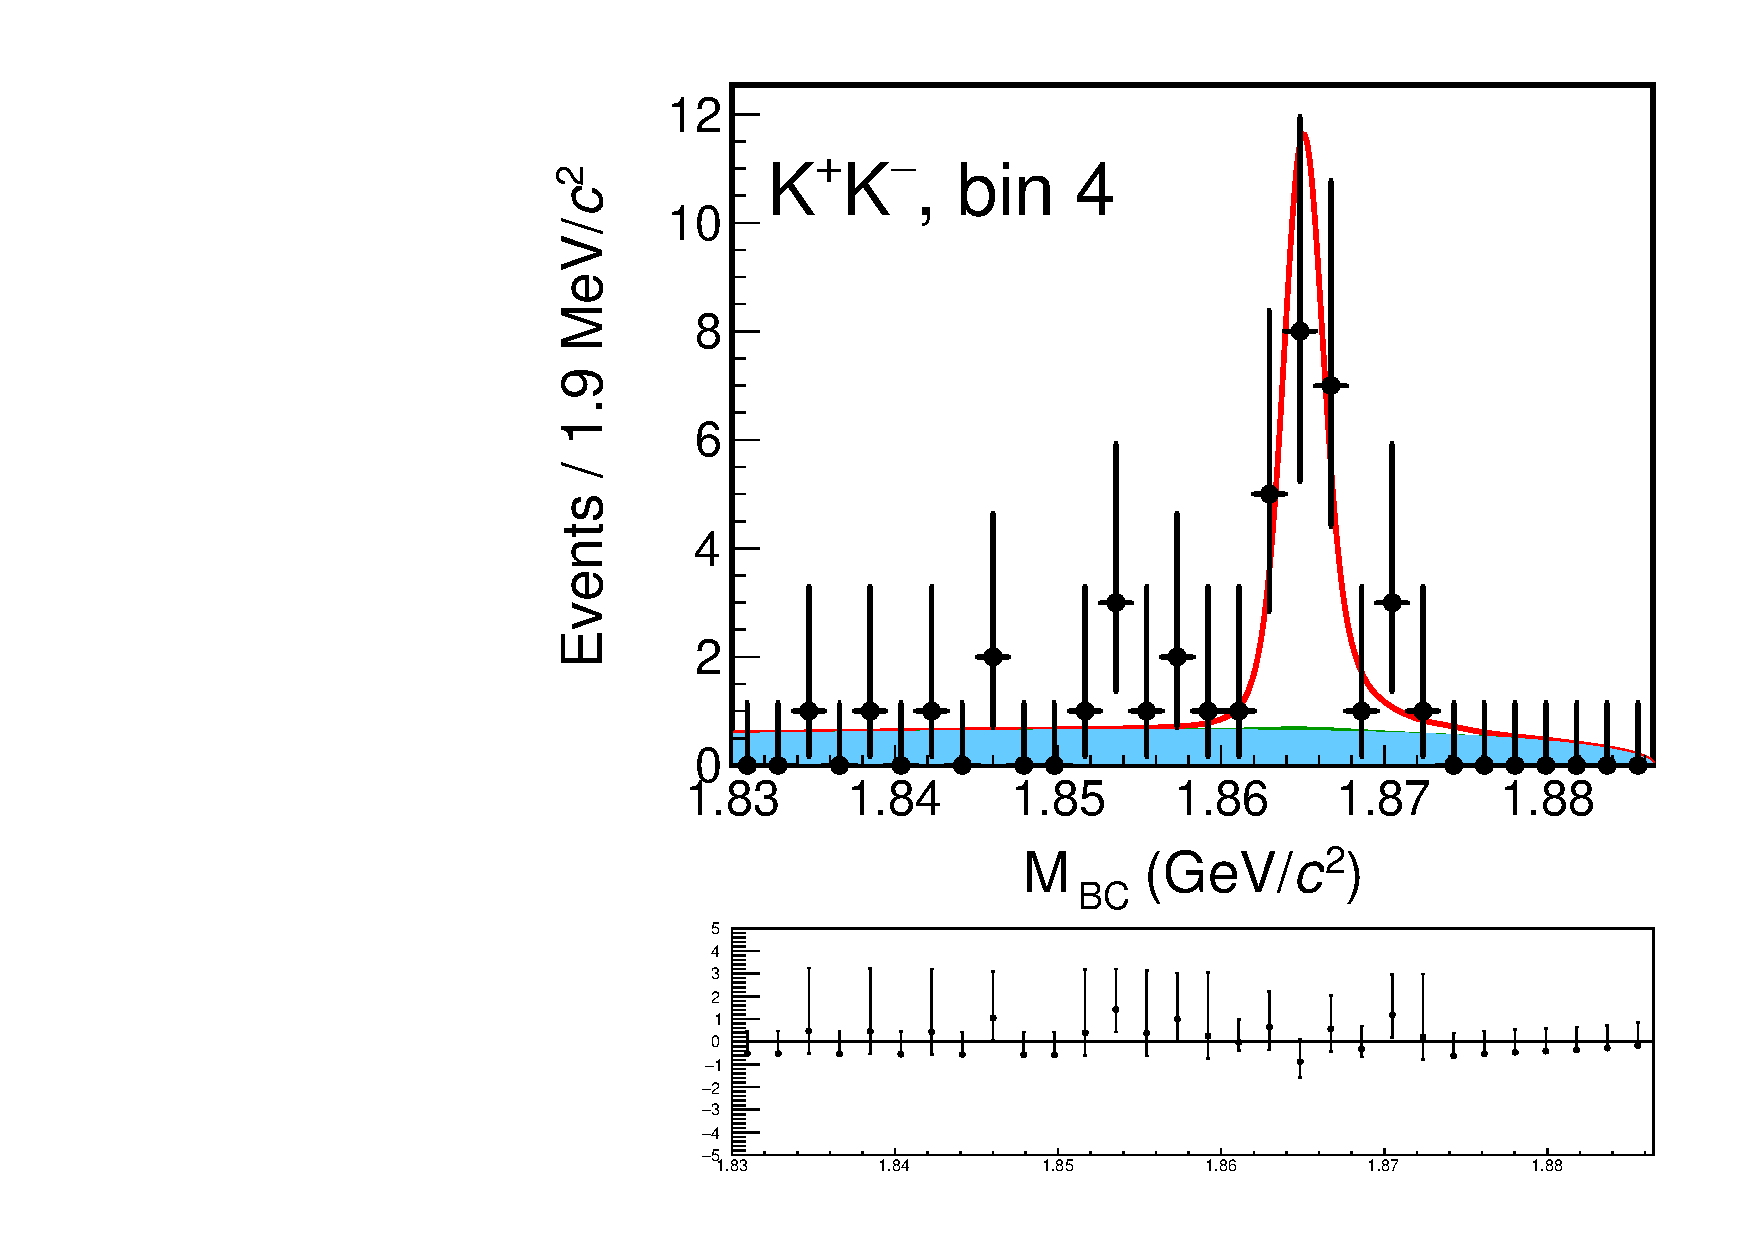
\includegraphics[width=0.75\textwidth,trim={0 5cm 0 0},clip=true]{Plots/DoubleTagYield_DoubleTag_CP_KKpipi_vs_KK_SignalBin4.pdf}
      \caption{Bin $4$ yield: $21.1_{-4.8}^{+5.5}$}
    \end{subfigure}
  \end{figure}
\end{frame}

\begin{frame}{Double tag fit of $KK\pi\pi$ vs $K_S\pi^0$}
  \begin{figure}
    \centering
    \begin{subfigure}{0.5\textwidth}
      \centering
      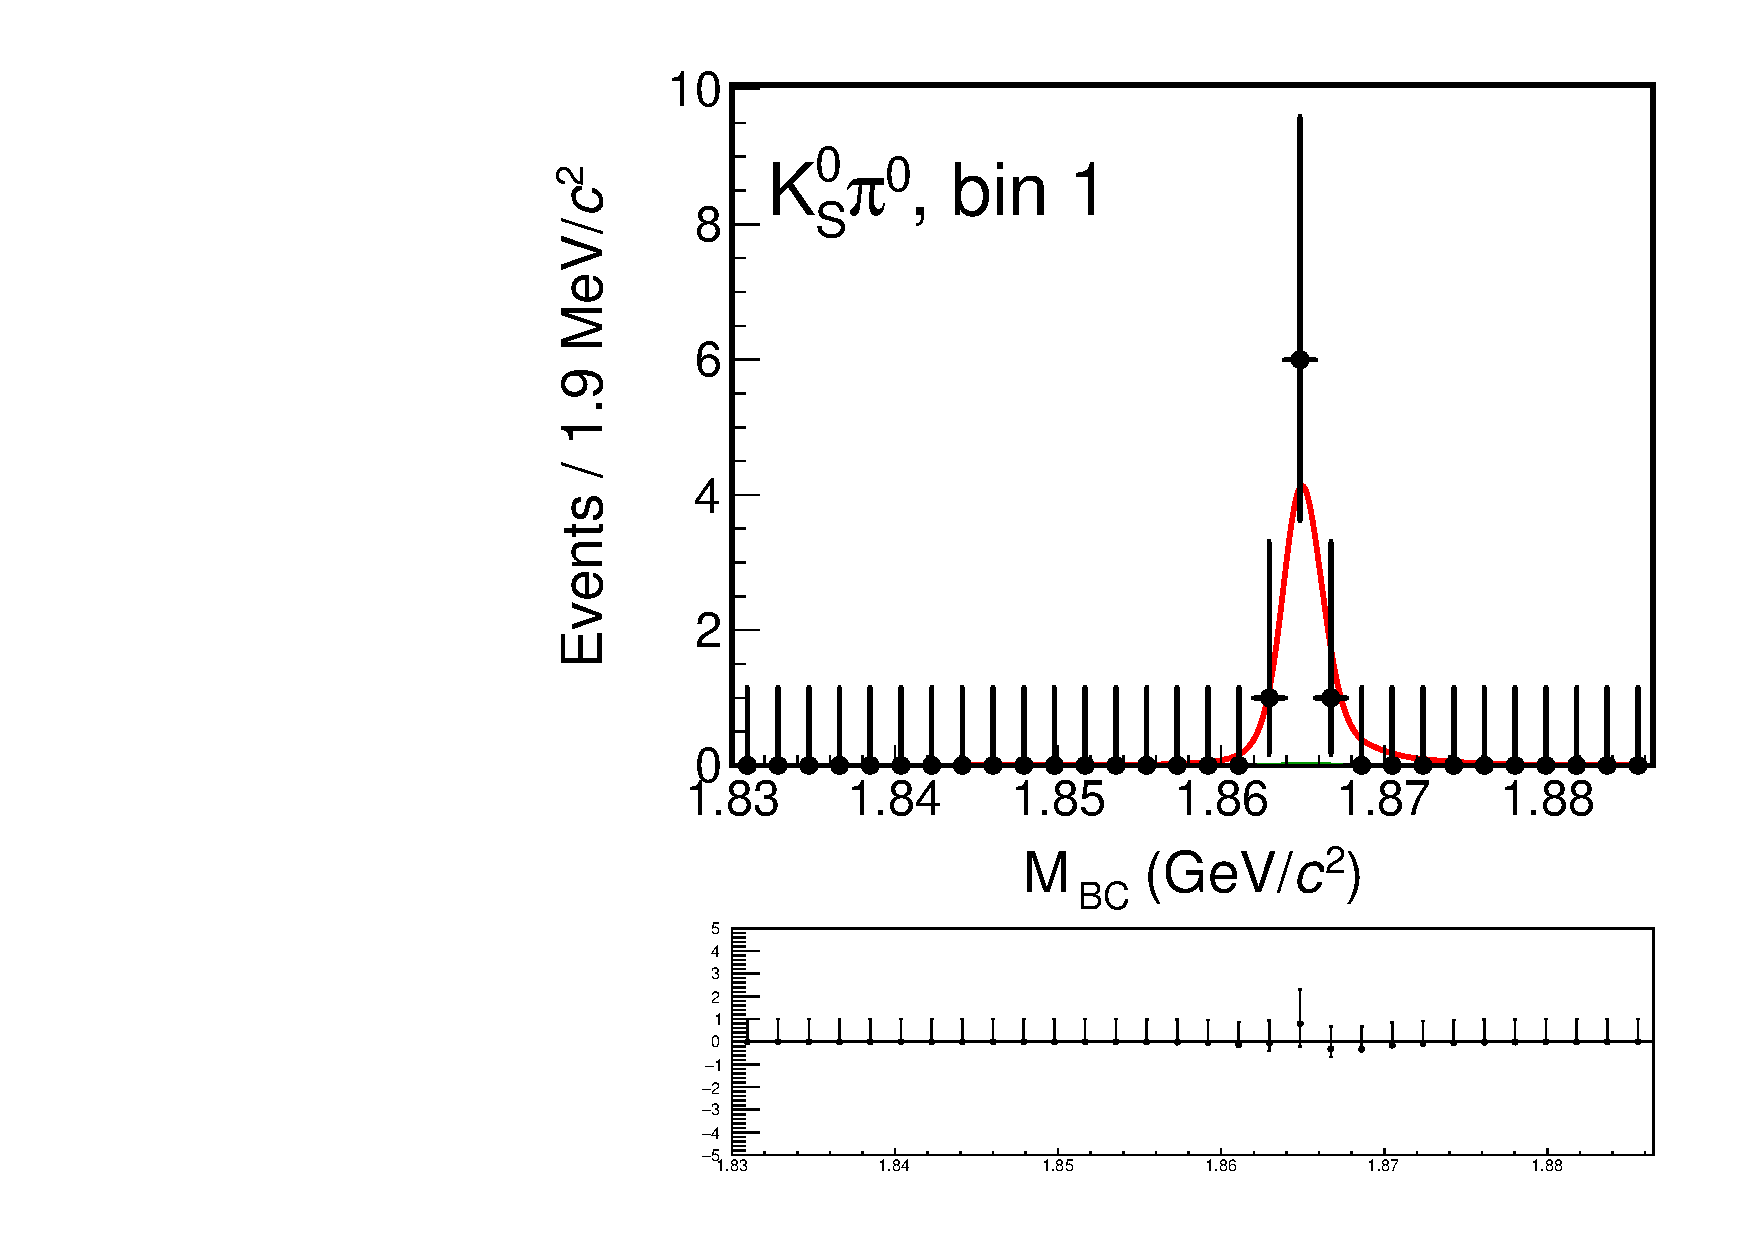
\includegraphics[width=0.75\textwidth,trim={0 5cm 0 0},clip=true]{Plots/DoubleTagYield_DoubleTag_CP_KKpipi_vs_KSpi0_SignalBin1.pdf}
      \caption{Bin $1$ yield: $7.9_{-2.5}^{+3.1}$}
    \end{subfigure}%
    \begin{subfigure}{0.5\textwidth}
      \centering
      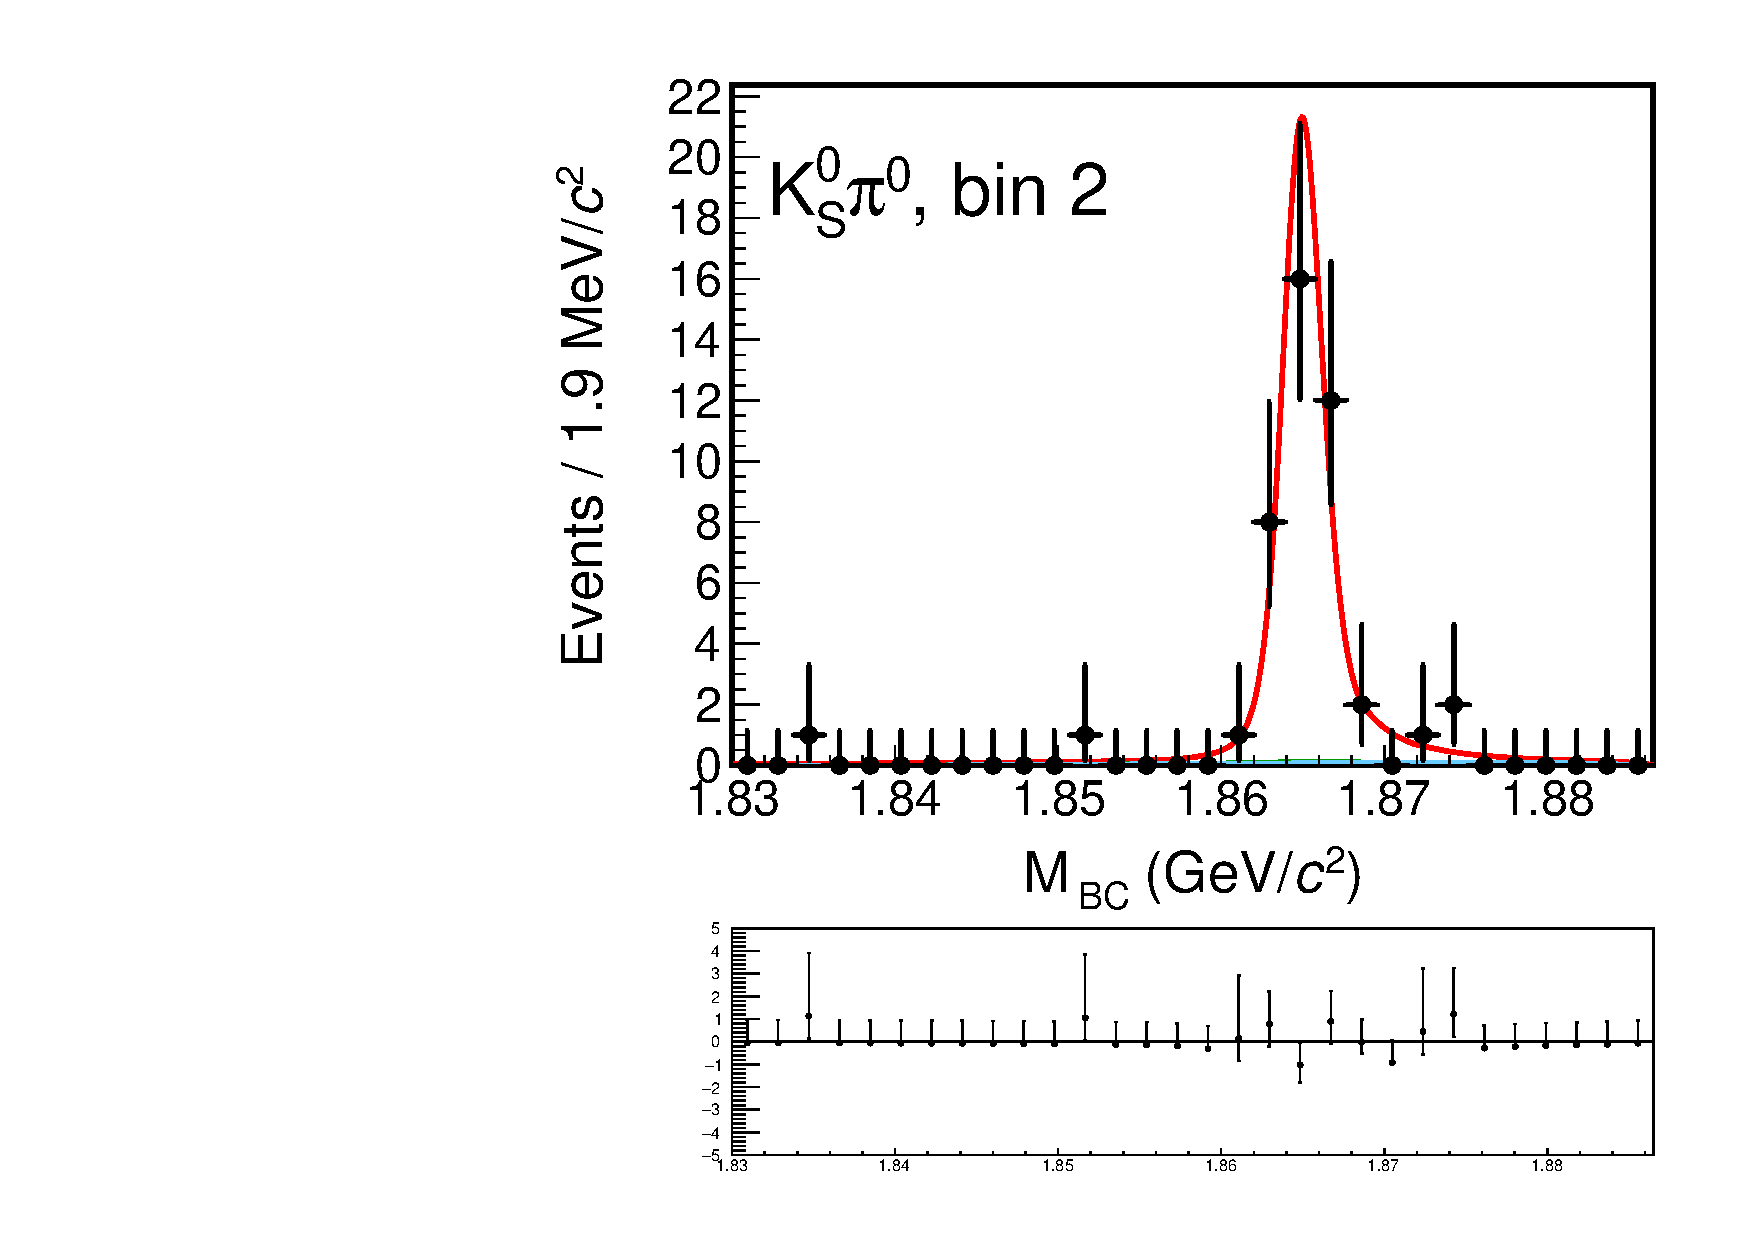
\includegraphics[width=0.75\textwidth,trim={0 5cm 0 0},clip=true]{Plots/DoubleTagYield_DoubleTag_CP_KKpipi_vs_KSpi0_SignalBin2.pdf}
      \caption{Bin $2$ yield: $40.4_{-6.3}^{+6.8}$}
    \end{subfigure}
    \begin{subfigure}{0.5\textwidth}
      \centering
      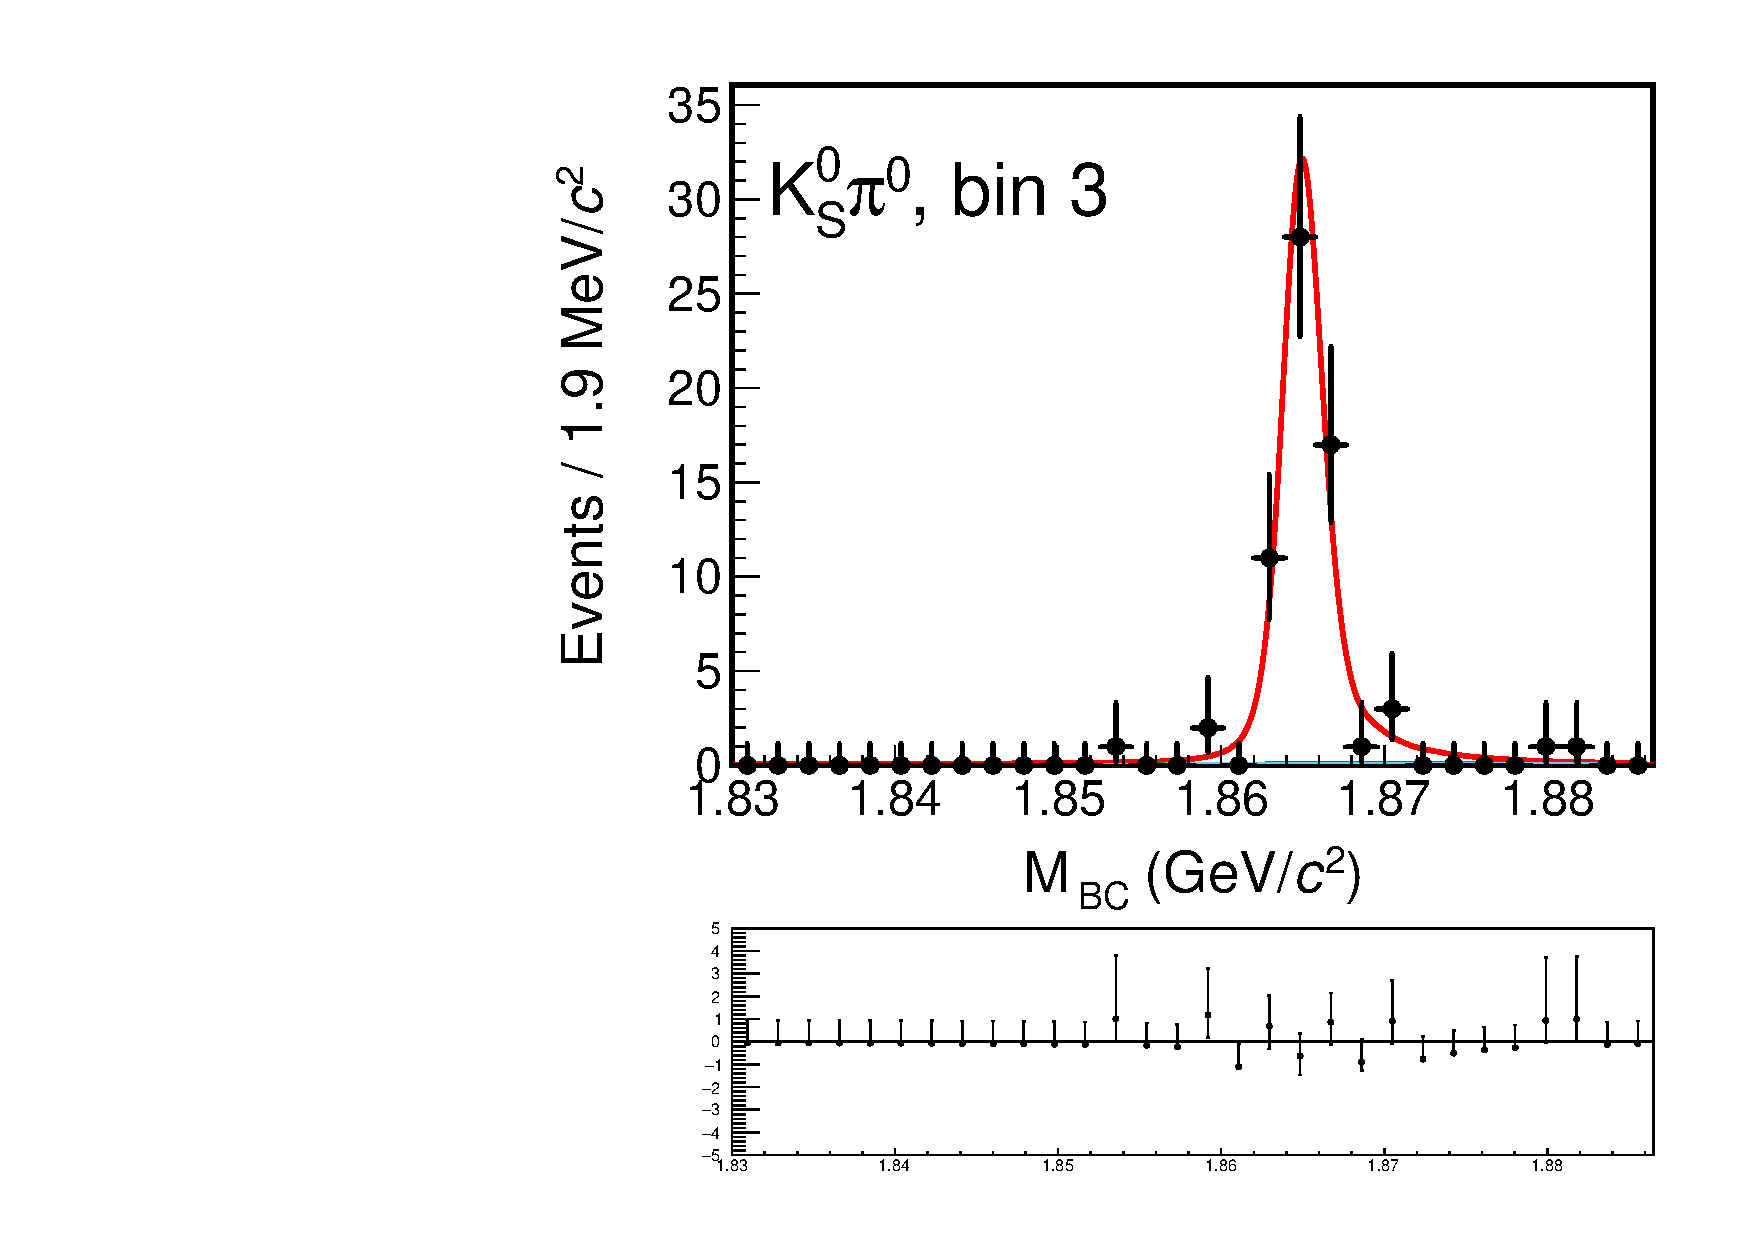
\includegraphics[width=0.75\textwidth,trim={0 5cm 0 0},clip=true]{Plots/DoubleTagYield_DoubleTag_CP_KKpipi_vs_KSpi0_SignalBin3.pdf}
      \caption{Bin $3$ yield: $61.1_{-7.8}^{+8.3}$}
    \end{subfigure}%
    \begin{subfigure}{0.5\textwidth}
      \centering
      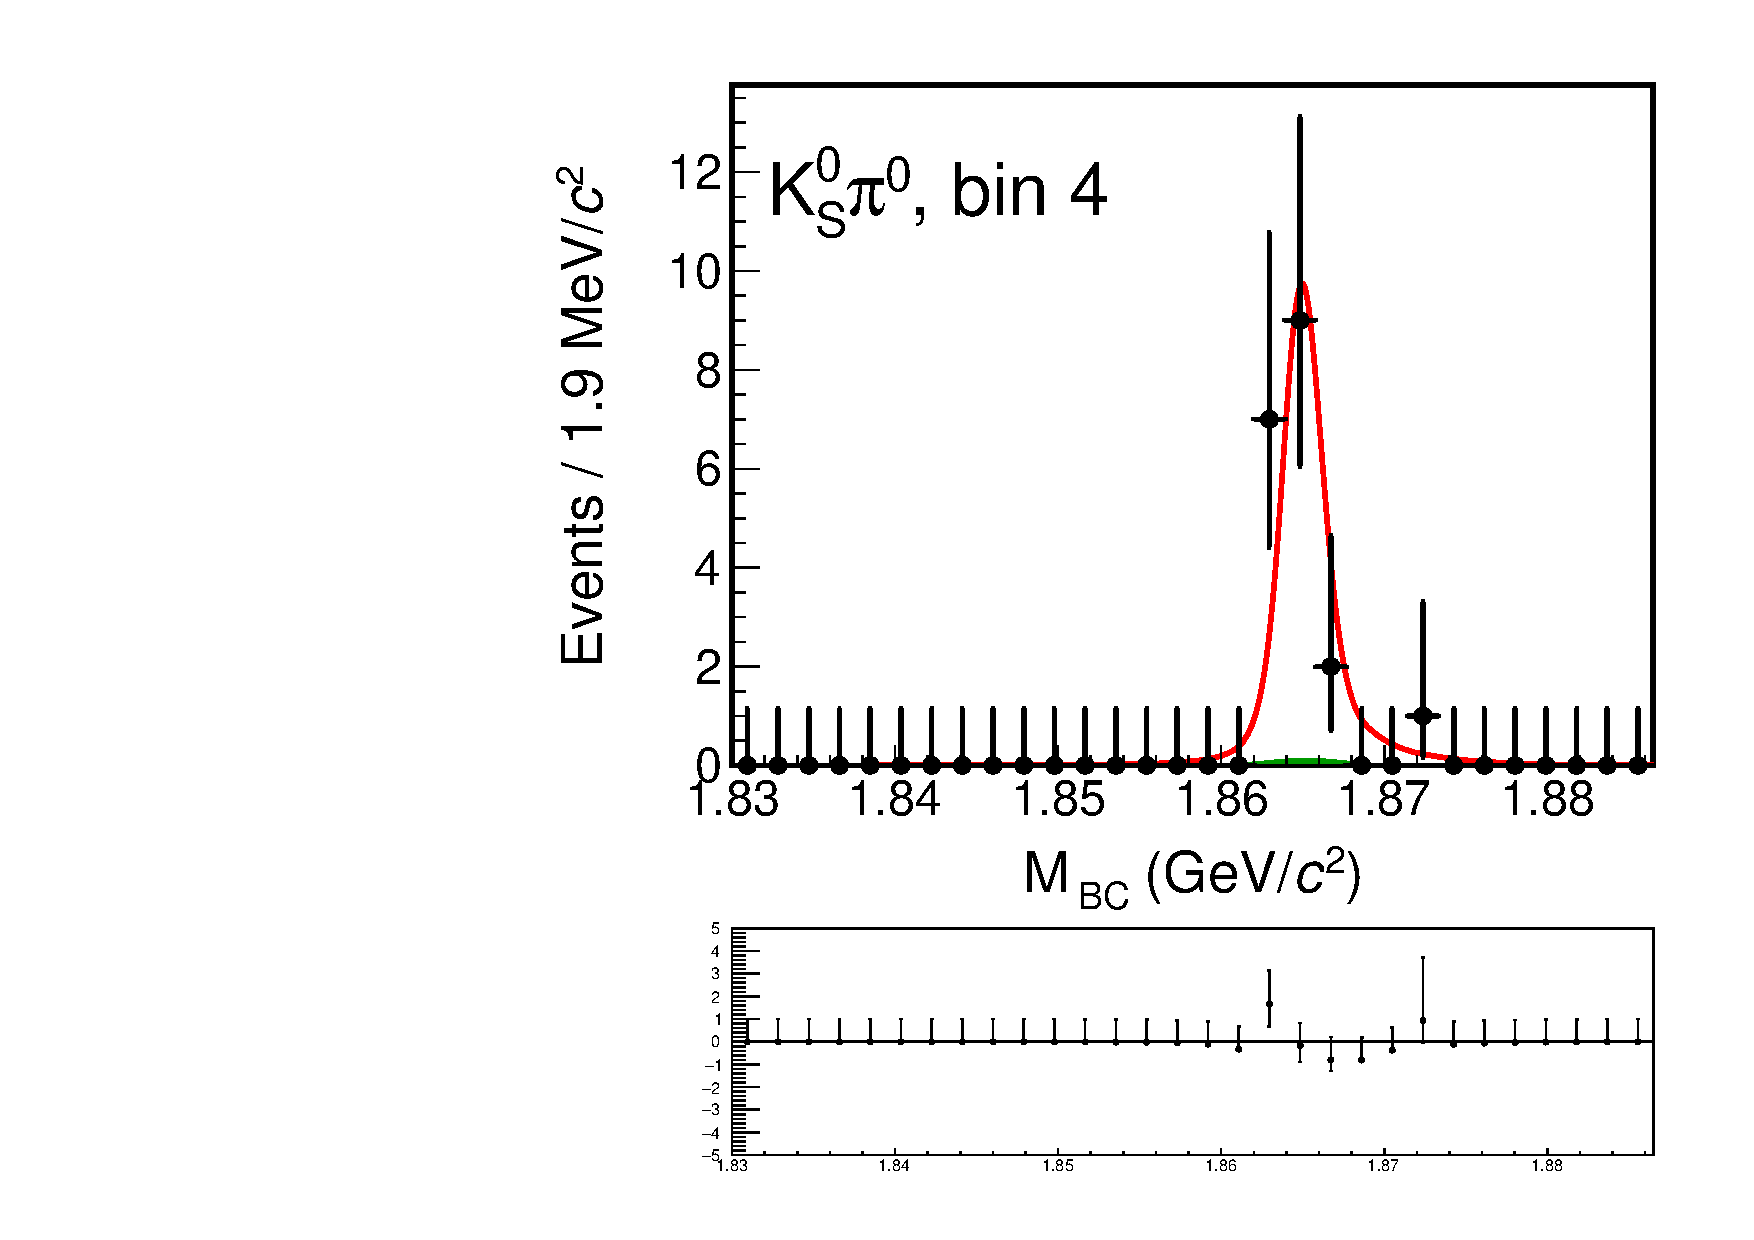
\includegraphics[width=0.75\textwidth,trim={0 5cm 0 0},clip=true]{Plots/DoubleTagYield_DoubleTag_CP_KKpipi_vs_KSpi0_SignalBin4.pdf}
      \caption{Bin $4$ yield: $18.3_{-3.9}^{+4.5}$}
    \end{subfigure}
  \end{figure}
\end{frame}

\begin{frame}{Double tag fit of partially reconstructed $KK\pi\pi$ vs $KK$}
  \begin{figure}
    \centering
    \begin{subfigure}{0.5\textwidth}
      \centering
      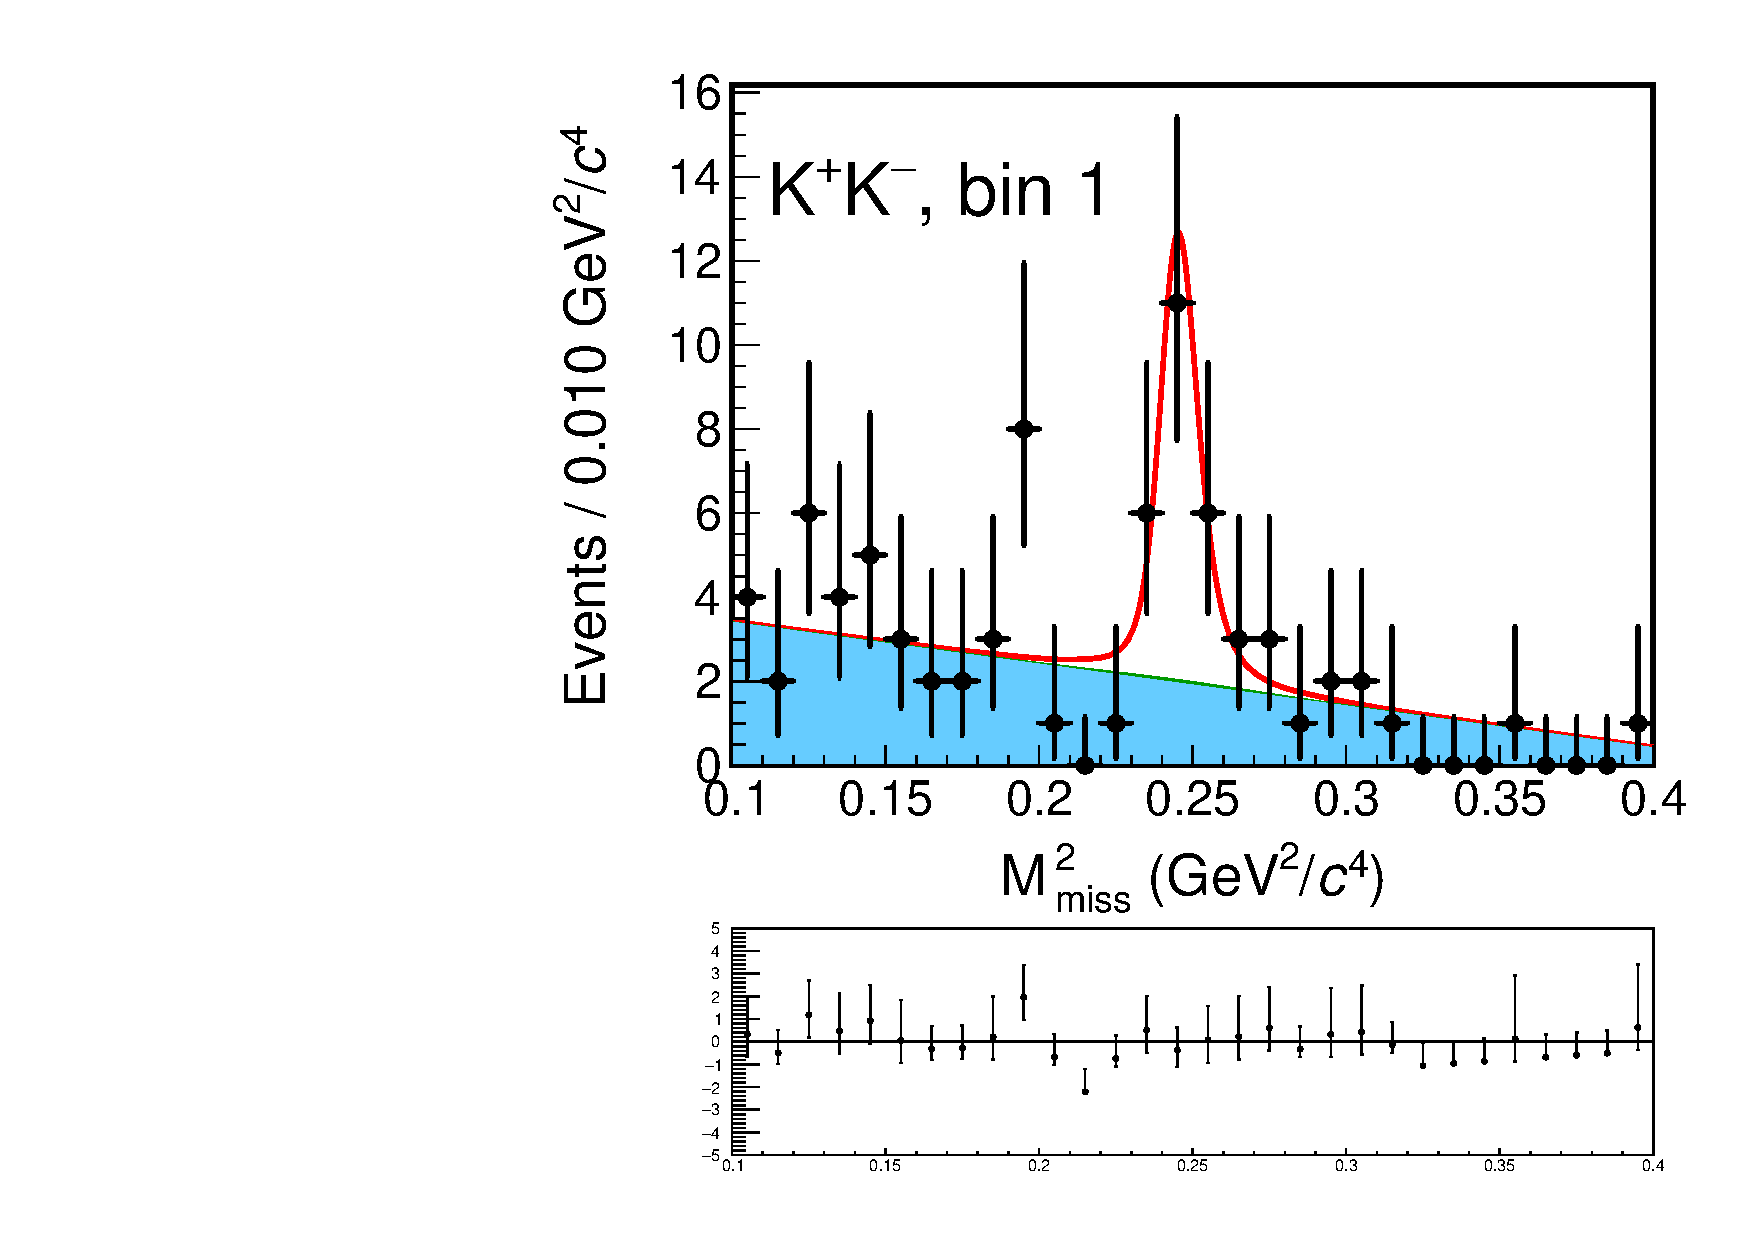
\includegraphics[width=0.75\textwidth,trim={0 5cm 0 0},clip=true]{Plots/DoubleTagYield_DoubleTag_CP_KKpipi_vs_KKPartReco_SignalBin1.pdf}
      \caption{Bin $1$ yield: $19.6_{-5.1}^{+5.8}$}
    \end{subfigure}%
    \begin{subfigure}{0.5\textwidth}
      \centering
      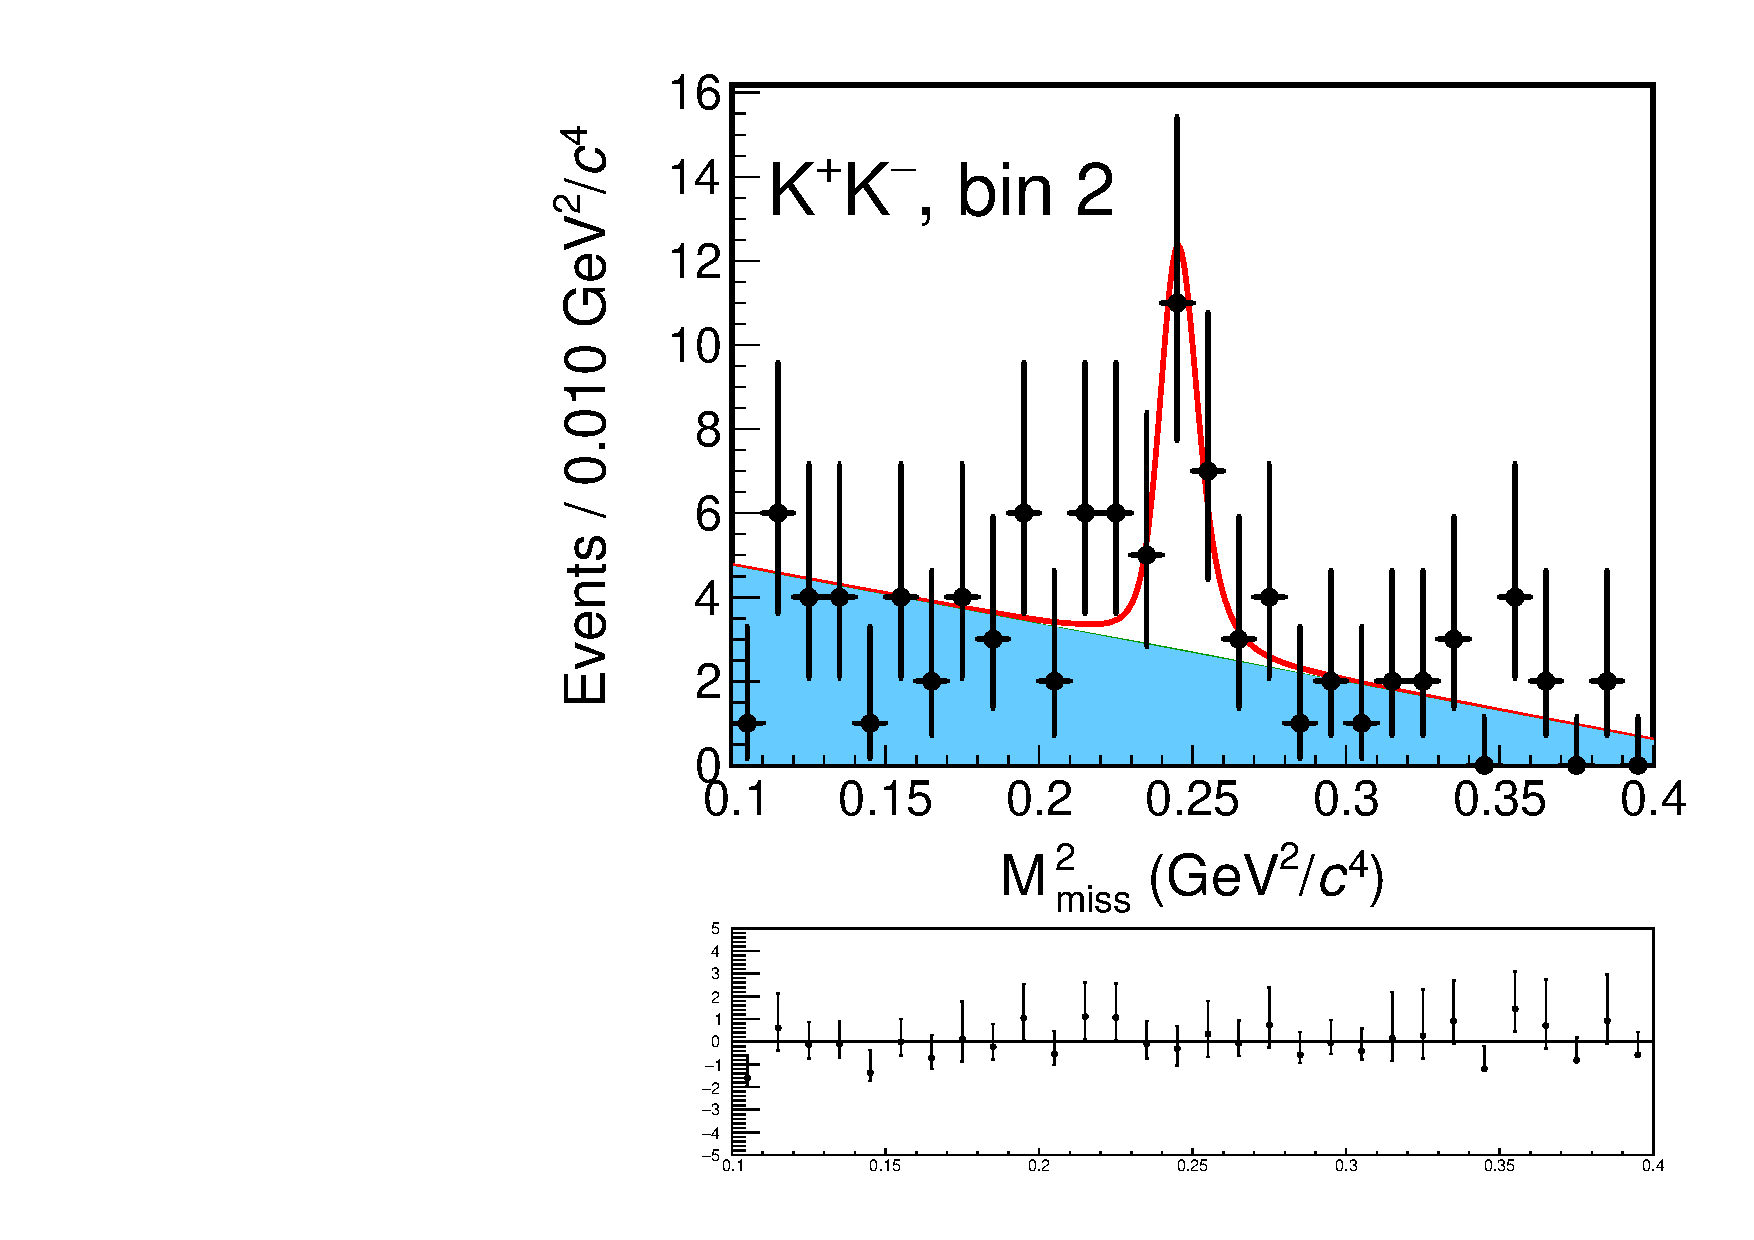
\includegraphics[width=0.75\textwidth,trim={0 5cm 0 0},clip=true]{Plots/DoubleTagYield_DoubleTag_CP_KKpipi_vs_KKPartReco_SignalBin2.pdf}
      \caption{Bin $2$ yield: $17.7_{-5.3}^{+6.1}$}
    \end{subfigure}
    \begin{subfigure}{0.5\textwidth}
      \centering
      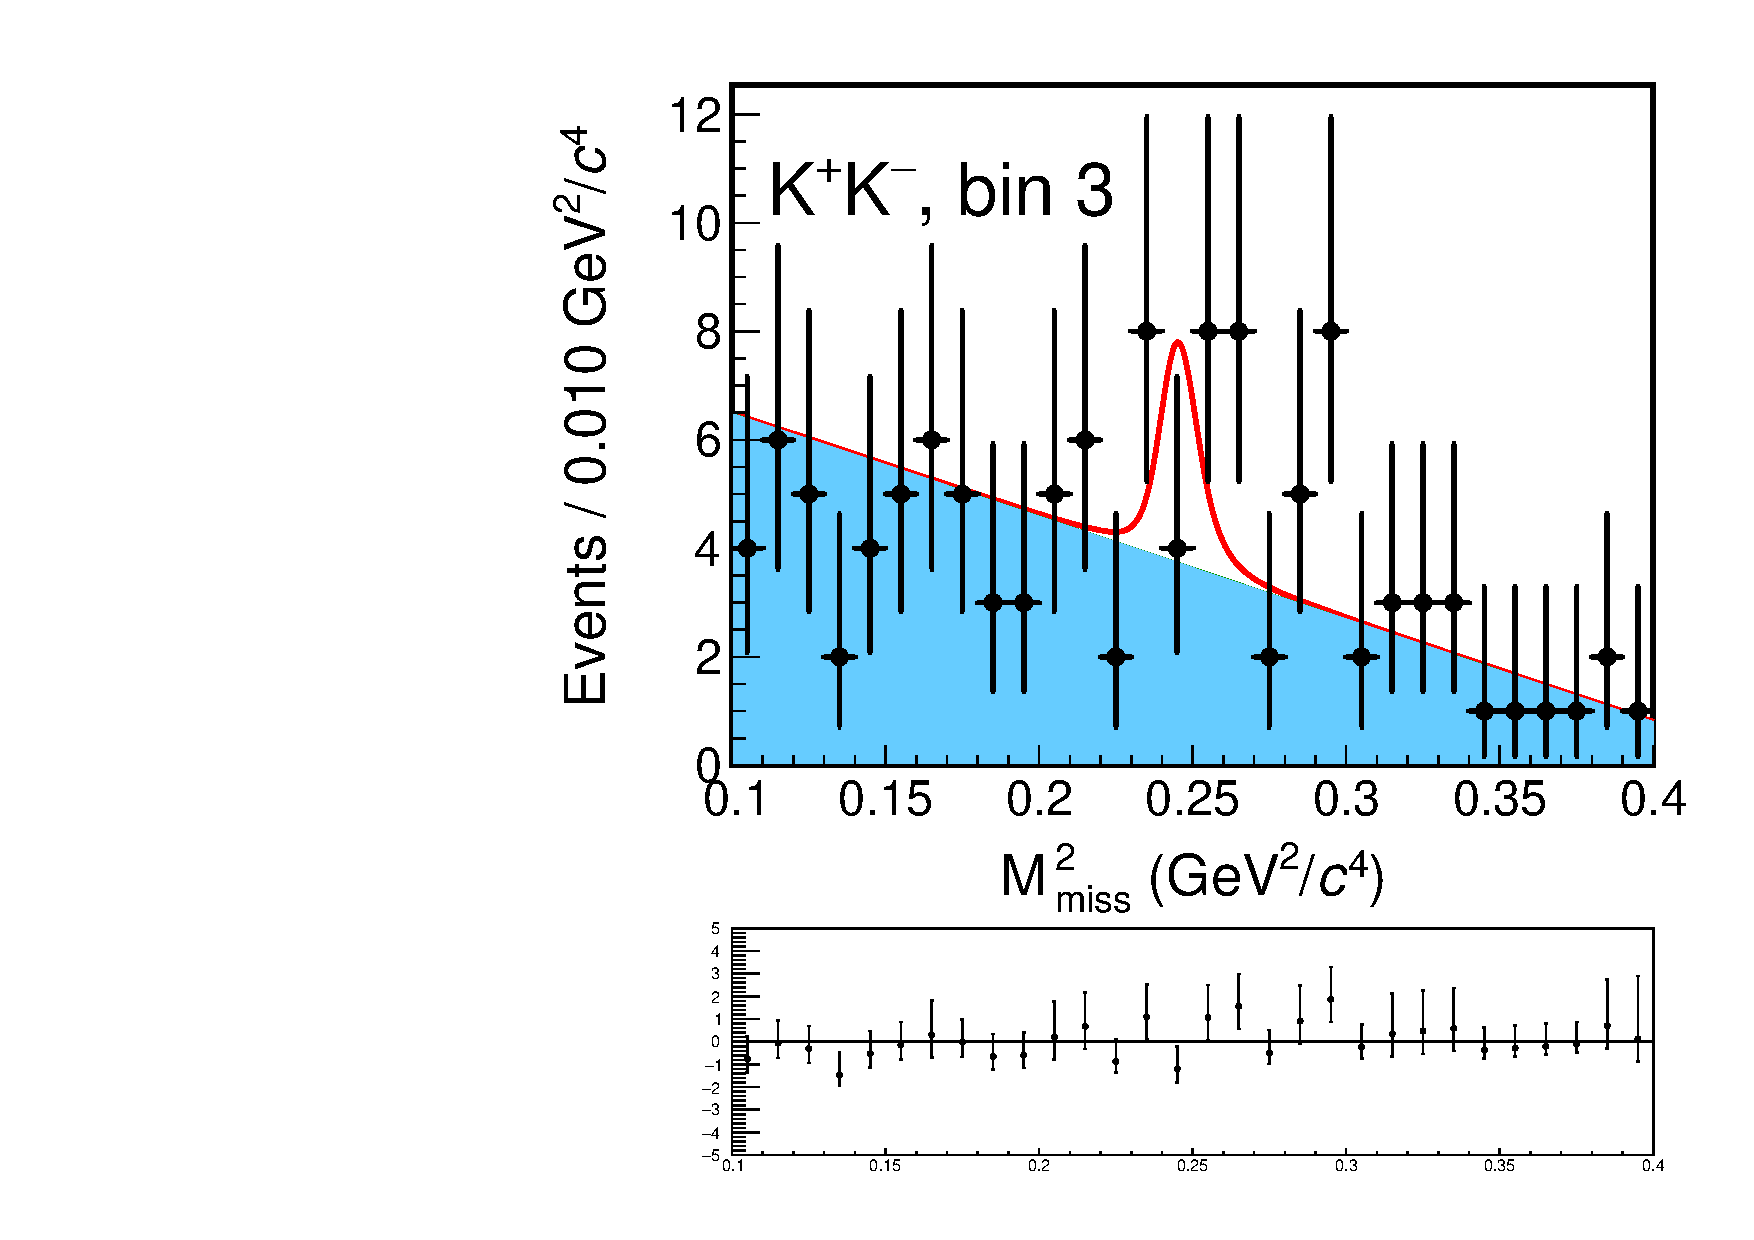
\includegraphics[width=0.75\textwidth,trim={0 5cm 0 0},clip=true]{Plots/DoubleTagYield_DoubleTag_CP_KKpipi_vs_KKPartReco_SignalBin3.pdf}
      \caption{Bin $3$ yield: $7.5_{-5.7}^{+6.6}$}
    \end{subfigure}%
    \begin{subfigure}{0.5\textwidth}
      \centering
      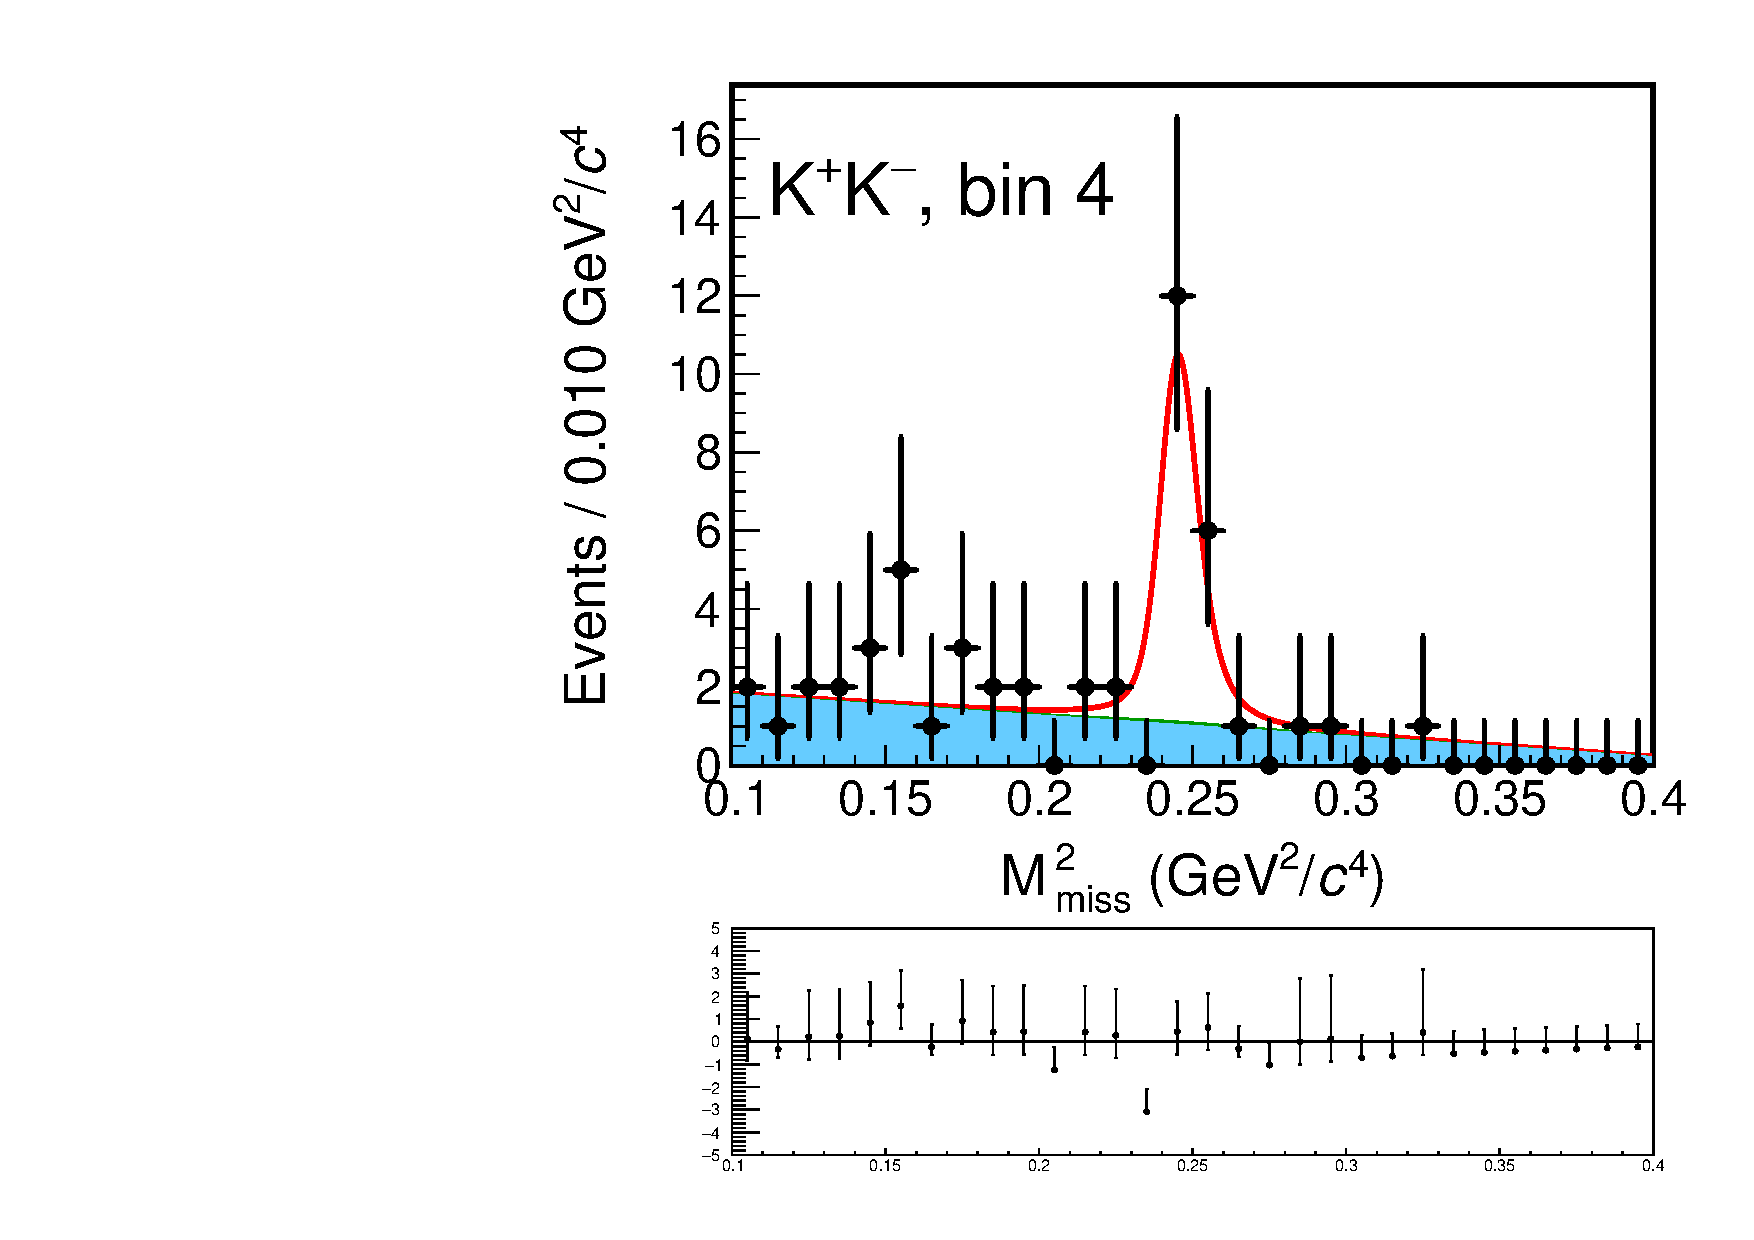
\includegraphics[width=0.75\textwidth,trim={0 5cm 0 0},clip=true]{Plots/DoubleTagYield_DoubleTag_CP_KKpipi_vs_KKPartReco_SignalBin4.pdf}
      \caption{Bin $4$ yield: $17.3_{-4.4}^{+5.1}$}
    \end{subfigure}
  \end{figure}
\end{frame}

\begin{frame}{Double tag fit of partially reconstructed $KK\pi\pi$ vs $K_S\pi^0$}
  \begin{figure}
    \centering
    \begin{subfigure}{0.5\textwidth}
      \centering
      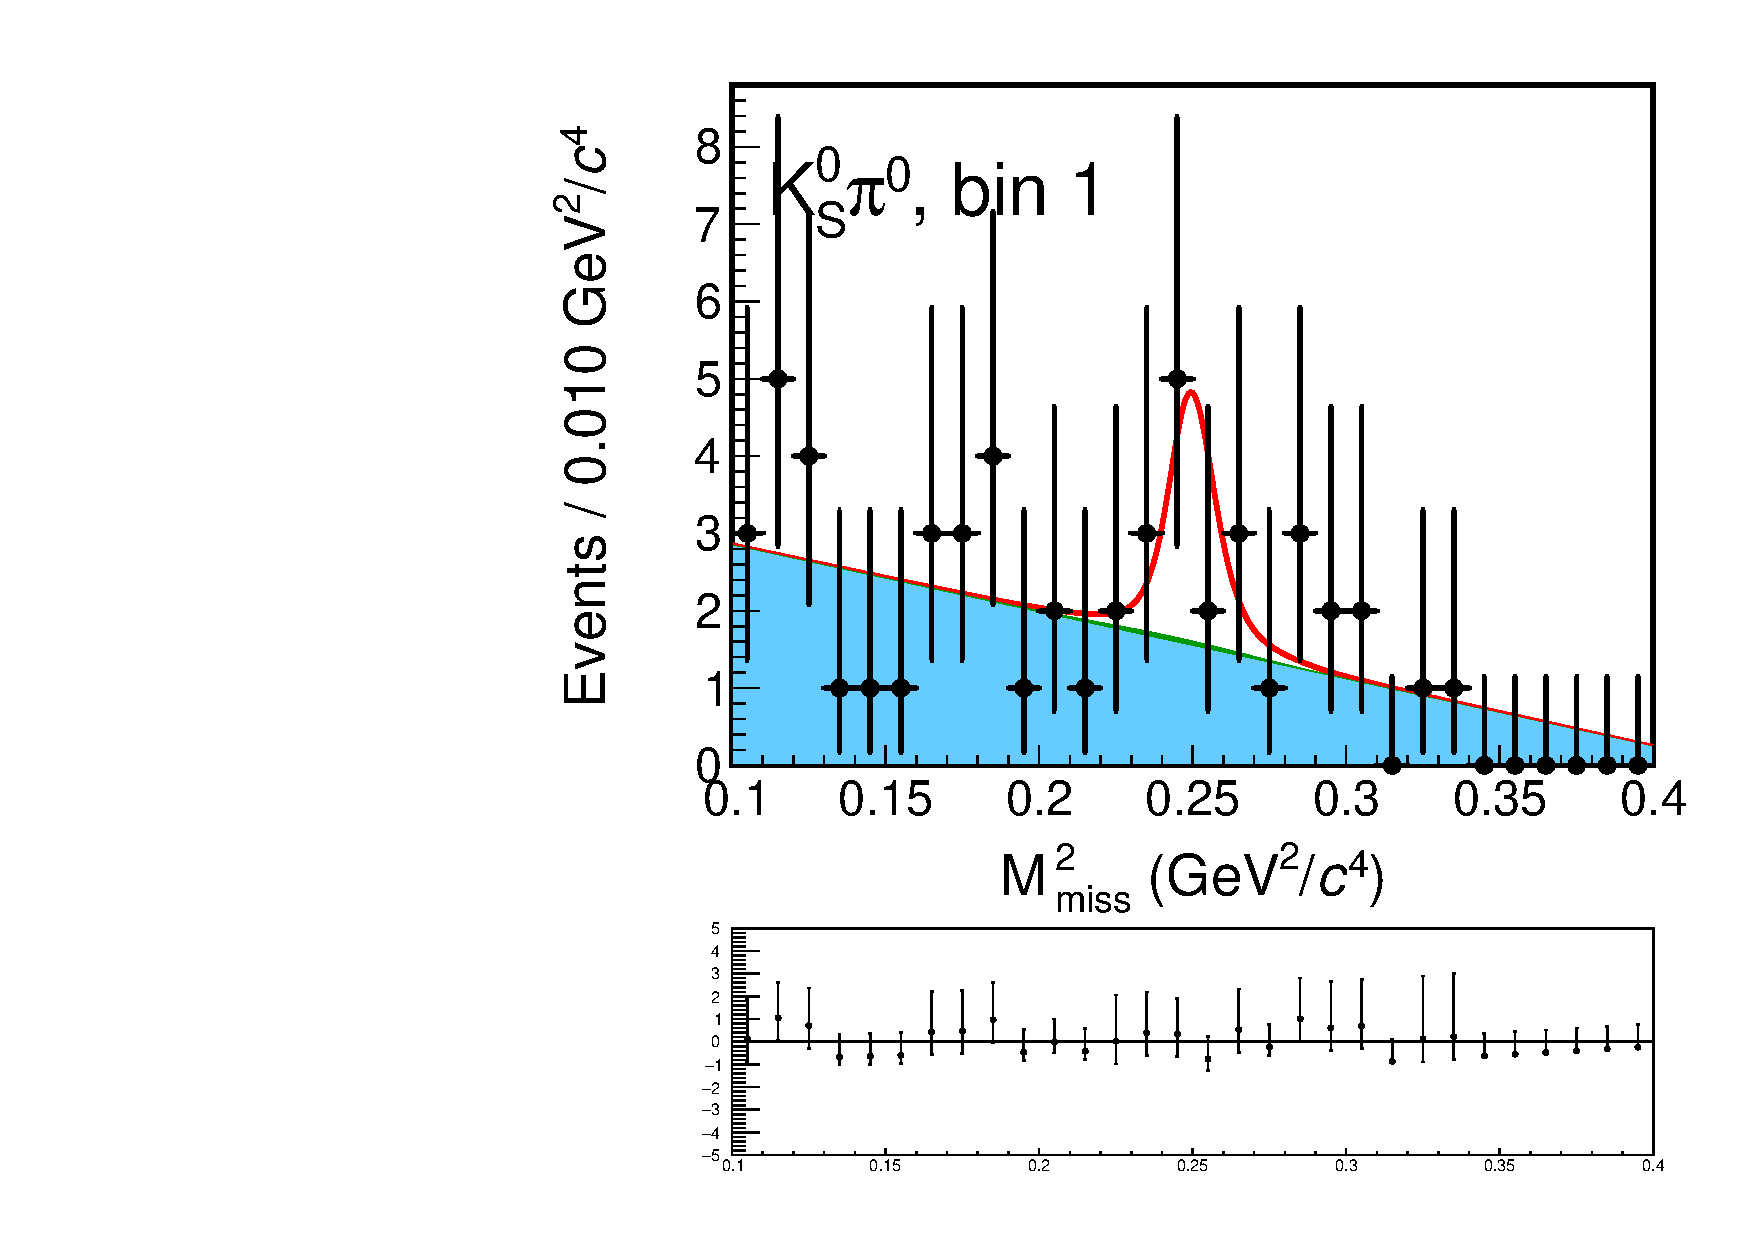
\includegraphics[width=0.75\textwidth,trim={0 5cm 0 0},clip=true]{Plots/DoubleTagYield_DoubleTag_CP_KKpipi_vs_KSpi0PartReco_SignalBin1.pdf}
      \caption{Bin $1$ yield: $7.2_{-3.5}^{+4.3}$}
    \end{subfigure}%
    \begin{subfigure}{0.5\textwidth}
      \centering
      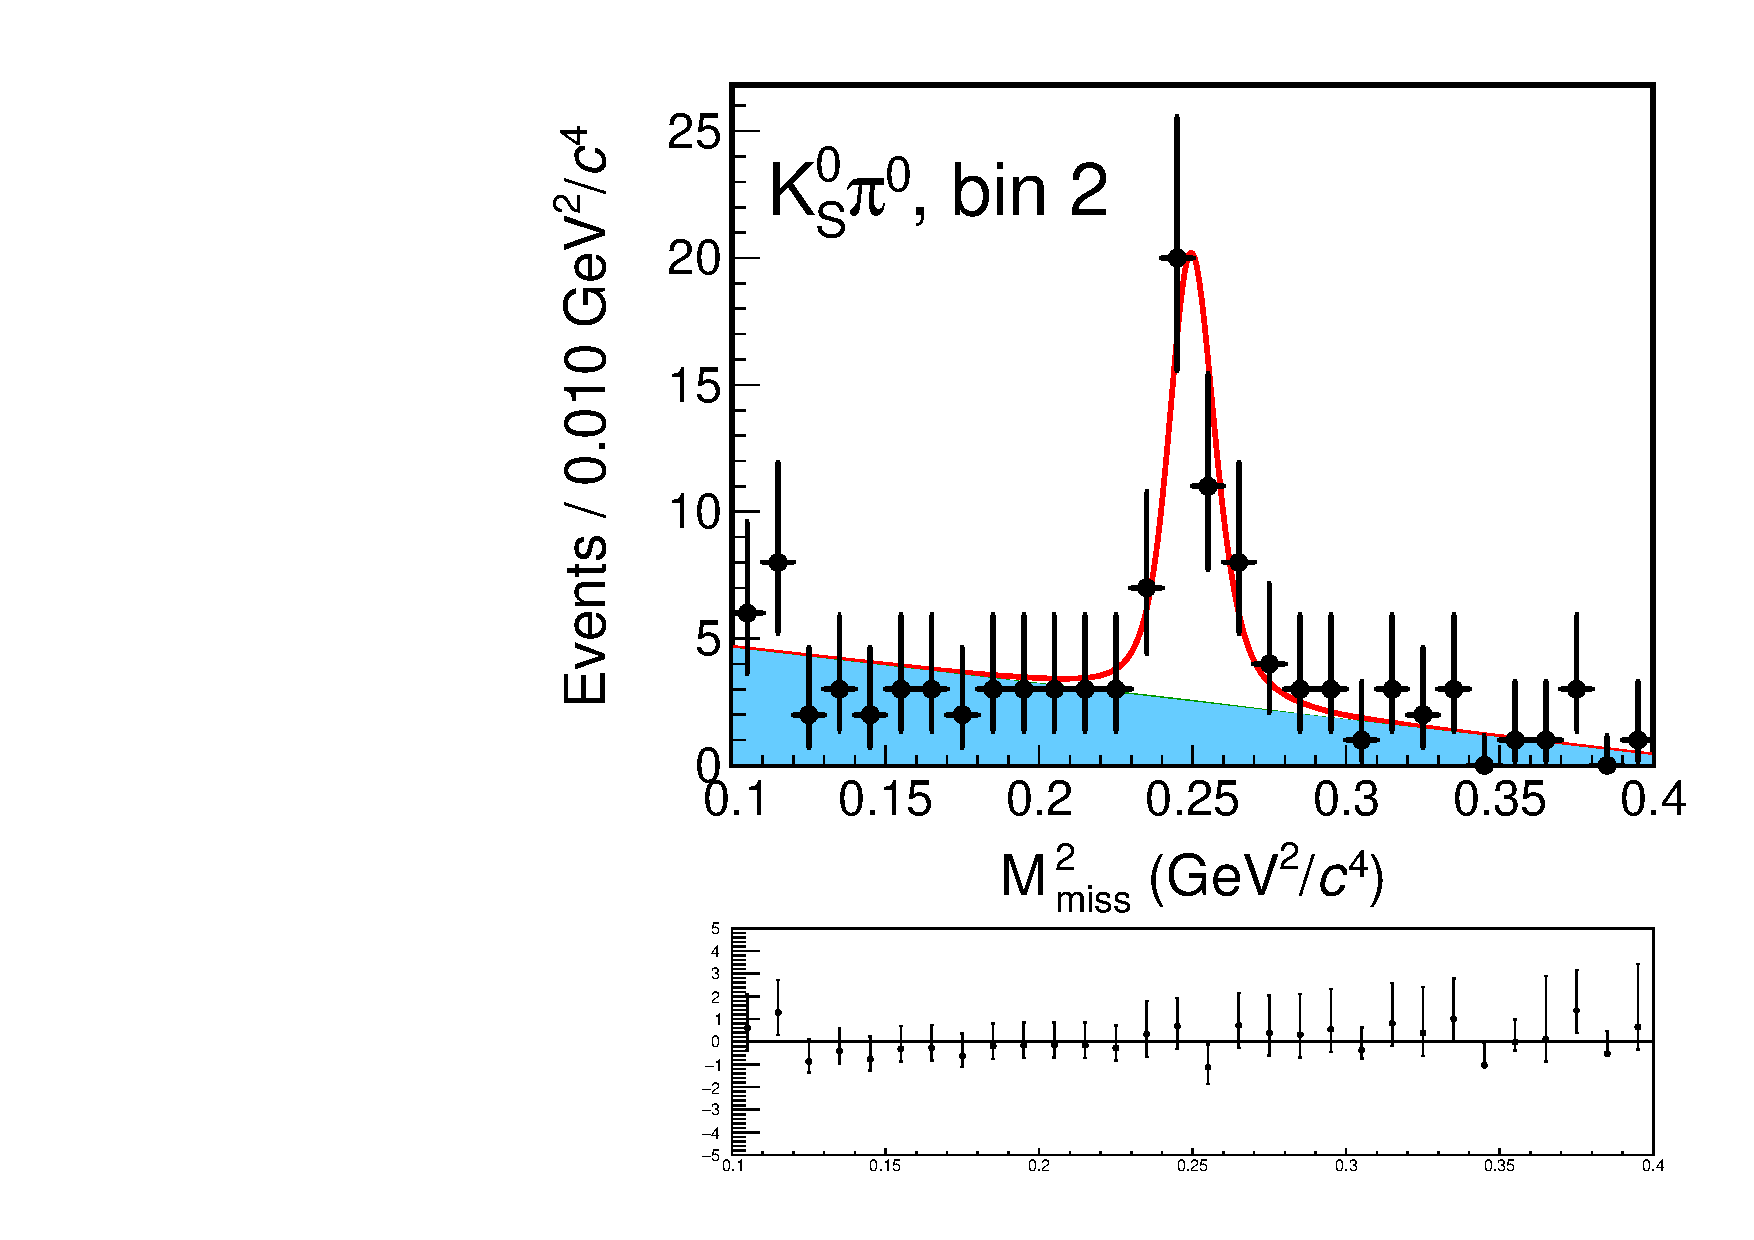
\includegraphics[width=0.75\textwidth,trim={0 5cm 0 0},clip=true]{Plots/DoubleTagYield_DoubleTag_CP_KKpipi_vs_KSpi0PartReco_SignalBin2.pdf}
      \caption{Bin $2$ yield: $39.3_{-7.3}^{+8.3}$}
    \end{subfigure}
    \begin{subfigure}{0.5\textwidth}
      \centering
      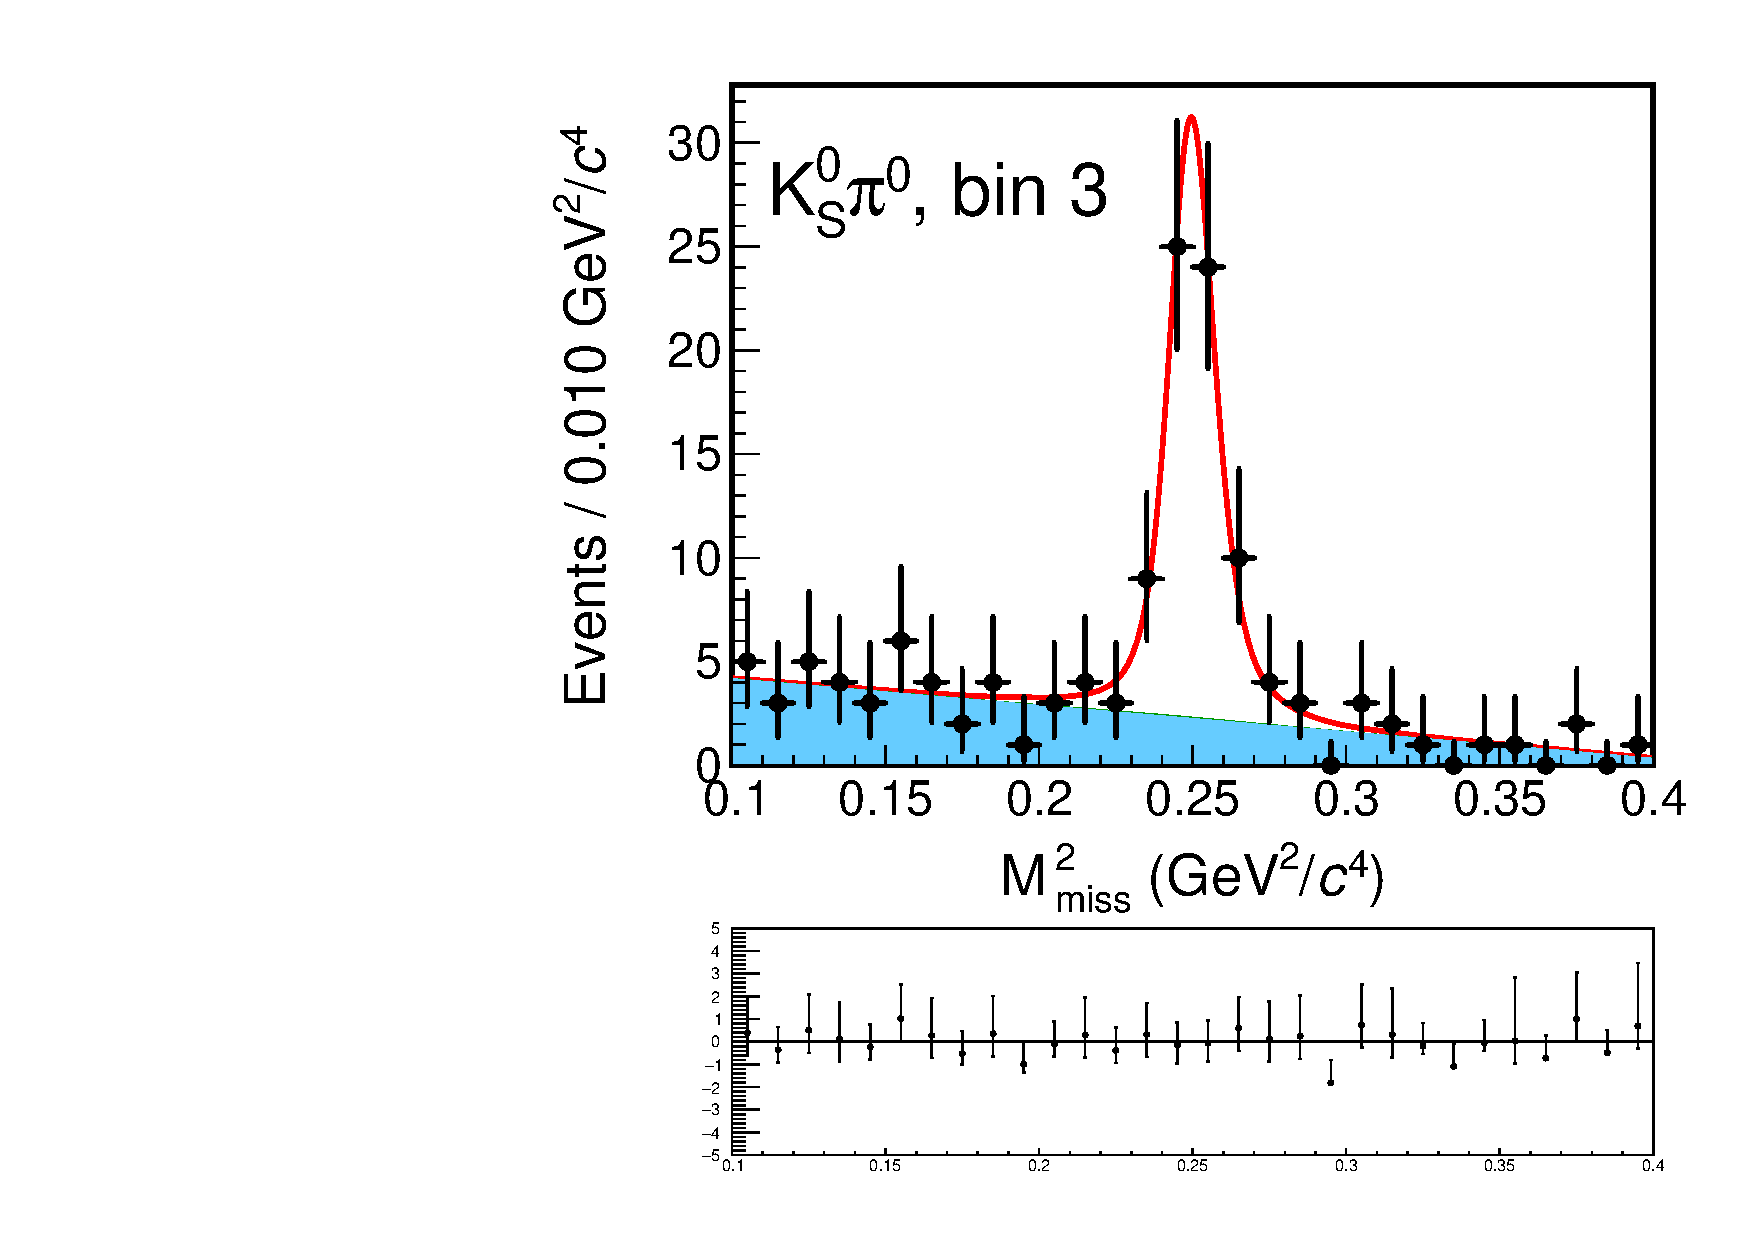
\includegraphics[width=0.75\textwidth,trim={0 5cm 0 0},clip=true]{Plots/DoubleTagYield_DoubleTag_CP_KKpipi_vs_KSpi0PartReco_SignalBin3.pdf}
      \caption{Bin $3$ yield: $64.4_{-9.0}^{+9.6}$}
    \end{subfigure}%
    \begin{subfigure}{0.5\textwidth}
      \centering
      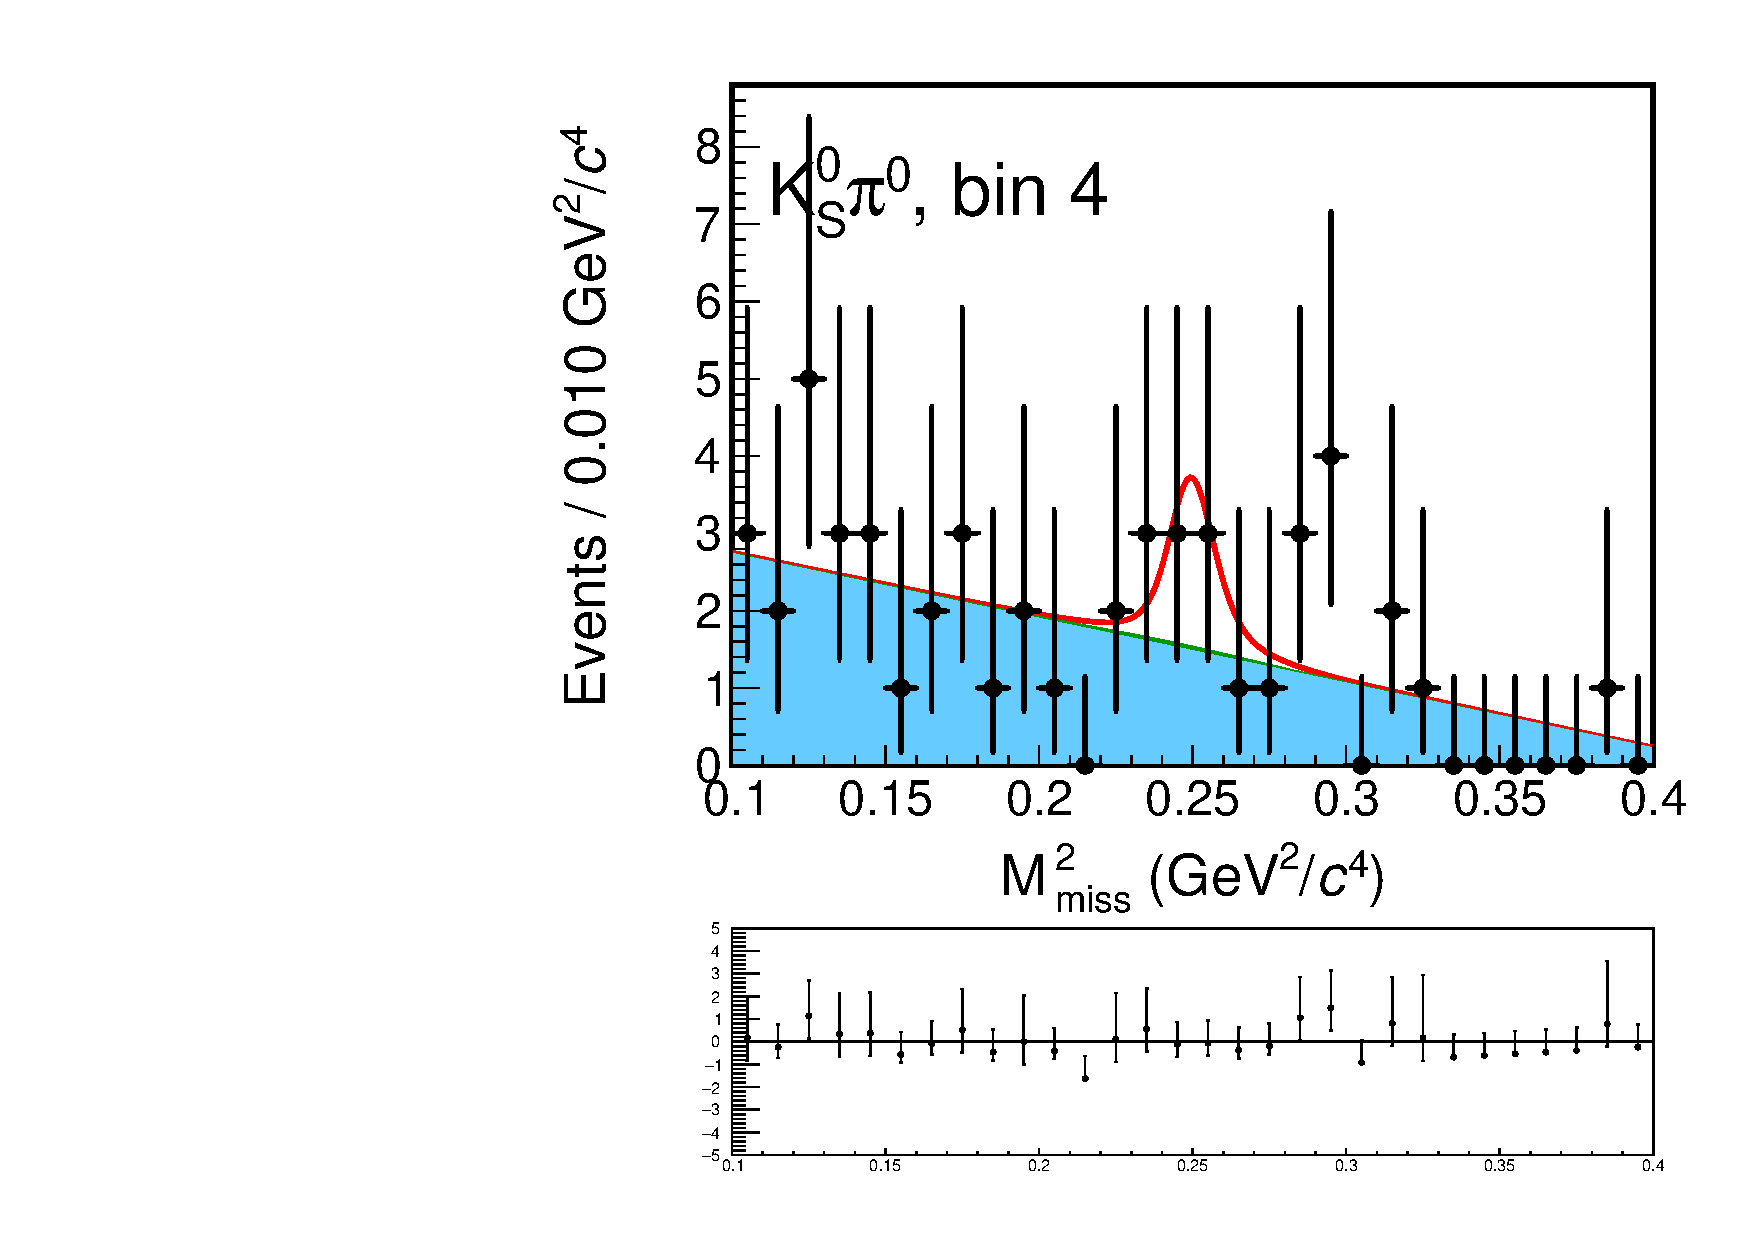
\includegraphics[width=0.75\textwidth,trim={0 5cm 0 0},clip=true]{Plots/DoubleTagYield_DoubleTag_CP_KKpipi_vs_KSpi0PartReco_SignalBin4.pdf}
      \caption{Bin $4$ yield: $4.8_{-3.0}^{+3.8}$}
    \end{subfigure}
  \end{figure}
\end{frame}

\section{Likelihood fit}
\begin{frame}{Likelihood fit}
  \vspace{0.0cm}
  {\Large How to put this all together to determine $c_i$ and $s_i$?}
  \begin{enumerate}
    \item{In the past, the strategy has been to measure normalised $K_i$ first, using flavour tags:}
  \end{enumerate}
  \begin{center}
    $\frac{N^{\rm DT}_i}{N^{\rm ST}}\propto K_i$, \quad$\sum_iK_i = 1$
  \end{center}
  \begin{enumerate}
    \setcounter{enumi}{1}
    \item{However, the $K_i$ must be corrected for efficiencies and bin migrations, in addition to Doubly Cabbibo Suppressed decays:}
  \end{enumerate}
  \begin{center}
    $f_i = \Big(1 + r_D^2\frac{K_{-i}}{K_i} - 2\sqrt{\frac{K_{-i}}{K_i}}\big(c_i\cos(\delta_D) + s_i\sin(\delta_D)\big)\Big)^{-1}$
  \end{center}
  \begin{enumerate}
    \setcounter{enumi}{2}
    \item{Finally, with the $K_i$ fixed, $c_i$ and $s_i$ are determined from CP and multi-body tags:}
  \end{enumerate}
  \begin{center}
    $\frac{N^{\rm DT}_i}{N^{\rm ST}}\propto K_i + K_{-i} \mp 2\sqrt{K_iK_{-i}}c_i$\\
    $\frac{N^{\rm DT}_{ij}}{N^{\rm ST}}\propto K_iK_{-j}^\prime + K_{-i}K_j^\prime - 2\sqrt{K_iK_{-i}K_j^\prime K_{-j}^\prime}(c_ic_j^\prime + s_is_j^\prime)$
  \end{center}
\end{frame}

\begin{frame}{Likelihood fit}
  \vspace{0.0cm}
  {\Large We propose a simpler, but perhaps powerful strategy:}
  \begin{enumerate}
    \item{Treat all $K_i$, $c_i$ and $s_i$ as free parameters}
    \item{Include the $D\to KK\pi\pi$ branching fraction $\mathcal{B}$ as a free parameter}
    \item{Fit flavour, $C\!P$ and multi-body tags simultaneously}
  \end{enumerate}
  \begin{center}
    {\Large Master equations:}
    \begin{align*}
      \hat{N}^{\rm DT}_i =& N^{\rm ST}\mathcal{B}\epsilon_{ij}\Big(K_{-j} + K_j - 2\sqrt{K_jK_{-j}}\big(c_j\cos(\delta_D) + s_j\sin(\delta_D)\big)\Big) \\
      \hat{N}^{\rm DT}_i =& N^{\rm ST}\mathcal{B}\epsilon_{ij}(K_j + K_{-j} \mp 2\sqrt{K_jK_{-j}}c_j) \\
      \hat{N}^{\rm DT}_{ij} =& N^{\rm ST}\mathcal{B}\epsilon_{ijkl}\big(K_{k}K_{-l}^\prime + K_{-k}K_{l}^\prime - 2\sqrt{K_{k}K_{-k}K_{l}^\prime K_{-l}^\prime}(c_{k}c_{l}^\prime + s_{k}s_{l}^\prime)\big)
    \end{align*}
  \end{center}
  \begin{center}
    $\epsilon_{ij}$ are combined efficiency and bin migration matrices\\~\\
    {\large The master equations use the free parameters $\mathcal{B}$, $K_i$, $c_i$ and $s_i$ to make a prediction $\hat{N}^{\rm DT}$ to the measured double tag yields $N^{\rm DT}$}
  \end{center}
\end{frame}

\begin{frame}{Likelihood fit}
  \begin{block}{Master equations}
    \begin{center}
      \vspace{-0.5cm}
      \begin{align*}
        \hat{N}^{\rm DT}_i =& N^{\rm ST}\mathcal{B}\epsilon_{ij}\Big(K_{-j} + K_j - 2\sqrt{K_jK_{-j}}\big(c_j\cos(\delta_D) + s_j\sin(\delta_D)\big)\Big) \\
        \hat{N}^{\rm DT}_i =& N^{\rm ST}\mathcal{B}\epsilon_{ij}(K_j + K_{-j} \mp 2\sqrt{K_jK_{-j}}c_j) \\
        \hat{N}^{\rm DT}_{ij} =& N^{\rm ST}\mathcal{B}\epsilon_{ijkl}\big(K_{k}K_{-l}^\prime + K_{-k}K_{l}^\prime - 2\sqrt{K_{k}K_{-k}K_{l}^\prime K_{-l}^\prime}(c_{k}c_{l}^\prime + s_{k}s_{l}^\prime)\big)
      \end{align*}
    \end{center}
  \end{block}
  \vspace{0.5cm}
  \begin{center}
    Ordinarily, we would construct a Gaussian (log)likelihood function $\implies$\\
    Obtain $\mathcal{B}$, $K_i$, $c_i$ and $s_i$ by minimising the following function\footnotetext{$\rho$ are correlation coefficients}:
    \begin{align*}
      -\ln(\mathcal{L}) =& \frac{1}{2}\sum_{\rm Tag}\sum_{ij}(V^{-1})_{ij}(N^{\rm DT}_i - \hat{N}^{\rm DT}_i)(N^{\rm DT}_j - \hat{N}^{\rm DT}_j) \\
      V_{ij} =& \rho_{ij}\sigma_i\sigma_j\phantom{, \quad \sigma_i = \sqrt{\sigma_-\sigma_+ - (\sigma_+ - \sigma_-)(N^{\rm DT}_i - \hat{N}^{\rm DT})}}
    \end{align*}
  \end{center}
\end{frame}

\begin{frame}{Likelihood fit}
  \begin{block}{Master equations}
    \begin{center}
      \vspace{-0.5cm}
      \begin{align*}
        \hat{N}^{\rm DT}_i =& N^{\rm ST}\mathcal{B}\epsilon_{ij}\Big(K_{-j} + K_j - 2\sqrt{K_jK_{-j}}\big(c_j\cos(\delta_D) + s_j\sin(\delta_D)\big)\Big) \\
        \hat{N}^{\rm DT}_i =& N^{\rm ST}\mathcal{B}\epsilon_{ij}(K_j + K_{-j} \mp 2\sqrt{K_jK_{-j}}c_j) \\
        \hat{N}^{\rm DT}_{ij} =& N^{\rm ST}\mathcal{B}\epsilon_{ijkl}\big(K_{k}K_{-l}^\prime + K_{-k}K_{l}^\prime - 2\sqrt{K_{k}K_{-k}K_{l}^\prime K_{-l}^\prime}(c_{k}c_{l}^\prime + s_{k}s_{l}^\prime)\big)
      \end{align*}
    \end{center}
  \end{block}
  \vspace{0.5cm}
  \begin{center}
    Our DT yields are very small, so their uncertainties are asymmetric $\implies$\\
    Approximate covariance matrix from the asymmetric uncertainties\footnote{\href{https://arxiv.org/abs/physics/0406120}{arXiv:physics/0406120}}:
    \begin{align*}
      -\ln(\mathcal{L}) =& \frac{1}{2}\sum_{\rm Tag}\sum_{ij}(V^{-1})_{ij}(N^{\rm DT}_i - \hat{N}^{\rm DT}_i)(N^{\rm DT}_j - \hat{N}^{\rm DT}_j) \\
      V_{ij} =& \rho_{ij}\sigma_i\sigma_j, \quad \sigma_i = \sqrt{\sigma_-\sigma_+ - (\sigma_+ - \sigma_-)(N^{\rm DT}_i - \hat{N}^{\rm DT})}
    \end{align*}
  \end{center}
\end{frame}

\begin{frame}{Likelihood fit}
  \vspace{-0.5cm}
  \begin{center}
    \begin{align*}
      -\ln(\mathcal{L}) =& \frac{1}{2}\sum_{\rm Tag}\sum_{ij}(V^{-1})_{ij}(N^{\rm DT}_i - \hat{N}^{\rm DT}_i)(N^{\rm DT}_j - \hat{N}^{\rm DT}_j) \\
      V_{ij} =& \rho_{ij}\sigma_i\sigma_j, \quad \sigma_i = \sqrt{\sigma_-\sigma_+ - (\sigma_+ - \sigma_-)(N^{\rm DT}_i - \hat{N}^{\rm DT})}
    \end{align*}
  \end{center}
  \begin{itemize}
    \setlength\itemsep{1.0em}
    \item{The above likelihood has good coverage for flavour and $C\!P$ tags...}
    \item{... but not for multi-body decays}
    \begin{itemize}
      \item{Bins with $\sigma_-\approx0$ make the fit unstable}
      \item{Fit convergence was found to be less than $60\%$}
    \end{itemize}
    \item{In multi-body decays, use the full unbinned likelihood directly}
    \begin{itemize}
      \item{Fit convergence improves to over $99\%$}
      \item{Much slower, but much more accurate}
    \end{itemize}
  \end{itemize}
\end{frame}

\section{Parameterisation of \texorpdfstring{$K_i$}{Ki}}
\begin{frame}{Parameterisation of $K_i$}
  \vspace{0.0cm}
  {\Large One last technical detail...}
  \begin{itemize}
    \item{There are $8$ $K_i$ parameters, but since $\sum_iK_i = 1$, only $7$ are independent}
    \item{We could set $K_4 = 1 - \sum_{i\neq4}K_i$, but such a parameterisation is unstable}
    \item{Use a recursive fraction parameterisation (\href{https://link.springer.com/article/10.1007/JHEP02(2021)169}{JHEP \textbf{2021} 169 (2021)})}
    \item{Recursive fractions $R_i$ are defined as:}
  \end{itemize}
  \begin{center}
    \begin{equation*}
      R_i \equiv
      \begin{cases}
        K_i, & i = -4 \\
        K_i/\sum_{j\geq i}K_j, & -4 < i < +4 \\
        1, &i = +4.
      \end{cases}
    \end{equation*}
  \end{center}
\end{frame}

\begin{frame}{Parameterisation of $K_i$}
  \vspace{0.0cm}
  \begin{center}
  {\large Visualisation of this parameterisation:}
  \end{center}
  \vspace{-0.3cm}
  \begin{center}
    \begin{block}{\centering 1. Definition of $c_1^\prime$}
      \begin{equation*}
        \underbrace{c_1}_{\equiv c_1^\prime} + \underbrace{c_2 + c_3 + ...}_{\equiv 1 - c_1^\prime} = 1
      \end{equation*}
    \end{block}
    \begin{block}{\centering 2. Eliminate $c_1$}
      \begin{equation*}
        c_2 + c_3 + c_4 + ... = 1 - c_1^\prime
      \end{equation*}
    \end{block}
    \begin{block}{\centering 3. Definition of $c_2^\prime$}
      \begin{equation*}
        \underbrace{\frac{c_2}{1 - c_1^\prime}}_{\equiv c_2^\prime} + \underbrace{\frac{c_3 + c_4 + ...}{1 - c_1^\prime}}_{\equiv 1 - c_2^\prime} = 1
      \end{equation*}
    \end{block}
    Repeat this procedure until the last coefficient, which is $1$
  \end{center}
\end{frame}

\section{Fit results}
\begin{frame}{Fit results}
\end{frame}

\section{Branching fraction measurement}
\begin{frame}{Branching fraction measurement}
\end{frame}

\section{Summary and conclusion}

\begin{frame}{Summary}
  \begin{itemize}
    \setlength\itemsep{1.0em}
    \item{A phase-space binned measurement of the $D^0\to K^+K^-\pi^+\pi^-$ strong-phases has been performed}
    \begin{itemize}
      \setlength\itemsep{0.7em}
      \item{Analysis uses a $2\times 4$ binning scheme}
      \item{Measurement will improve significantly with full $\SI{20}{\per\femto\barn}$ dataset}
      \item{New strategy: Treat $c_i$, $s_i$ and $K_i$ on an equal footing}
      \item{Additionally, $\delta_D^{K\pi}$ can also be determined}
      \item{The $D^0\to K^+K^-\pi^+\pi^-$ branching fraction is almost $3$ times more precise than the current PDG value}
    \end{itemize}
    \item{Next steps:}
    \begin{enumerate}
      \setlength\itemsep{0.7em}
      \item{Perform systematics studies}
      \item{Write up MEMO}
    \end{enumerate}
  \end{itemize}
  \begin{center}
    {\huge Thank you!}
  \end{center}
\end{frame}

\begin{frame}{Backup}
  \begin{center}
    {\huge Backup}
  \end{center}
\end{frame}

\renewcommand*{\thefootnote}{\fnsymbol{footnote}}
\begin{frame}{Tag modes}
  \begin{itemize}
    \setlength\itemsep{1.0em}
    \item{Flavour tags:}
    \begin{itemize}
      \item{$K\pi$, $K\pi\pi^0$, $K\pi\pi\pi$, $Ke\nu$}
    \end{itemize}
    \item{CP even tags:}
    \begin{itemize}
      \item{\underline{$KK$}, $\pi\pi$, \underline{$\pi\pi\pi^0$}\footnote{Mostly CP even}, $K_S\pi^0\pi^0$, $K_L\pi^0$}
    \end{itemize}
    \item{CP odd tags:}
    \begin{itemize}
      \item{\underline{$K_S\pi^0$}, $K_S\eta$, $K_S\pi\pi\pi^0$\footnote{Predominantly CP odd}, $K_S\eta^\prime_{\pi\pi\eta}$, $K_S\eta^\prime_{\rho\gamma}$}
    \end{itemize}
    \item{Self-conjugate tags:}
    \begin{itemize}
      \item{\underline{$K_S\pi\pi$}, $K_L\pi\pi$}
    \end{itemize}
  \end{itemize}
  \vspace{0.5cm}
  Underlined tags are also reconstructed with a missing kaon in $KK\pi\pi$
\end{frame}

\end{document}
